
\chapter{Linear Algebra: Maths of Deep Learning}

\lstset{language=python}          

$$
\newcommand\bs[1]{\boldsymbol{#1}}
\newcommand\norm[1]{\left\lVert#1\right\rVert}
$$


\section{Vector}
\label{sec:math-vectors}

\textcolor{red}{Using vector is important as it enables us to encapsulate any
representation (e.g. image, time series, electronic health-record) in the form
of a vector}.

\subsection{Row vs. Column vector}

Fundamentally, a vector is a list of numbers such as the Python \textcolor{blue}{\bf list} below.
\begin{lstlisting}{lang="python"}
# using list
x = [1, 5, 1]

# using numpy.array or       (has more built-in operations)
# better with numpy.ndarray (has more built-in operations, 
#   		handle any dimension)
myvector = np.array([3, 6, 9, 12])
myvector/3.0
print(myvector)

# shape (1, 3)
>>> a
array([1, 2, 3])

>>> a.transpose()
array([1, 2, 3])

>>> myvector.ndim
1

>>> myvector.shape
(3,)
\end{lstlisting}

The vector you are creating, using \verb!np.array!, is neither row nor column. It actually has 1 dimension only. You can verify that by
{\tiny
\begin{verbatim}
checking the number of dimensions myvector.ndim which is 1

checking the myvector.shape, which is (3,) (a tuple with one element only). 
	For a row vector is should be (1, 3), and for a column (3, 1)
\end{verbatim}
}

Mathematically, this can be written in the form of either row vector or column vector.
\textcolor{red}{The default orientation of a single vector is a {\bf column vector}}

\begin{enumerate}
  \item {\bf row vector}: mathematically, we use $x^T$ to indicate a row vector.
  
In Python, we create a row vector  using \textcolor{blue}{\bf np.array}
(numpy.array), or (better - expandable to higher dimension like matrix)
\textcolor{blue}{\bf np.ndarray} (numpy.ndarray).

OPTION 1: Use double square bracket, i.e. [[ ]], when writing your row vector.

\begin{lstlisting}
a = np.array([[1, 2, 3]])
\end{lstlisting}

OPTION 2: use the shortcut
\begin{lstlisting}
row = np.r_['r', [1,2,3]]     # shape: (1, 3)
\end{lstlisting}

OPTION 3: convert from a (column) vector
\begin{lstlisting}
row = my_vector.reshape(1, -1)
\end{lstlisting}

OPTION 4: use \verb!ndmin! option with value 2, when creating the vector
\begin{lstlisting}
>>> a = np.array([12, 3, 4, 5], ndmin=2)
>>> print a.shape
  (1,4)
  
\end{lstlisting}

  \item {\bf column vector}: mathematically, we use the notation \verb!x! to indicate a column vector. 


In Python, we create a column vector  using \textcolor{blue}{\bf np.array}
(numpy.array), or (better) \textcolor{blue}{\bf np.ndarray} (numpy.ndarray).

OPTION 1: pass explicitly

\begin{lstlisting}
column = np.array([  # 3 rows, with each row is 1-element list
    [1],
    [2],
    [3]
])
\end{lstlisting}

OPTION 2: convert from row vector, using either \verb!T! attribute or \verb!reshape()! method
\begin{lstlisting}
row_vector = array([[1, 2, 3]])

col_vector = row_vector.T  # shape (3, 1)

>>> a.transpose()


# or
column = row_vector.reshape(-1, 1)
\end{lstlisting}
where the -1 automatically finds the value of n (i.e. the exact number of elements).


OPTION 3: force it to be a column vector in Python by adding another dimension to the array

\verb!np.newaxis! to increase the one more dimension, when used once, i.e. 1D
array will become 2D array; 2D array will become 3D array.
So, we apply on an ndarray vector, make it a column vector by adding an axis
along the second dimension
\begin{lstlisting}
>>> a = np.arange(4)  # a vector with element from 0 to (n-1)
[0,1,2,3]

>>> a[:, np.newaxis]
array([[1],
       [2],
       [3]])
>>> a[np.newaxis, :]
array([[1, 2, 3]])
\end{lstlisting}


OPTION 4: use shortcut
\begin{lstlisting}
column = np.r_['c', [1,2,3]]  # shape: (3,1)
\end{lstlisting}

\end{enumerate}



\subsection{(Column) Vector: Direction vs. Point}

The default representation is a column vector, \verb!x! vector is a column
vector. However, this convention is opposite when using in matrix
(Sect.\ref{sec:math-matrix}).
\begin{equation}
x = [2, 4]^T
\end{equation}

Two common geometric interpretations of vectors, as either points or directions in space. 
\begin{itemize}
  \item points: 
  
 \textcolor{red}{Points provide an abstract way to classify a real-world
 problem}, e.g.
 pictures as either cats or dogs, we can start considering tasks abstractly as
 collections of points in space and picturing the task as discovering how to
 separate two distinct clusters of points.
 
 
The vector $x=[2,3]^T$ can be viewed  as the location 2 units to the right and 3
units up from the origin.
  
  \item direction: starting from the origin (0,0) to the point of the given coordinate.
  
The vector $x=[2,3]^T$ can be viewed  as the direction: take 2 steps to the right and 3
steps up.


  One of the benefits of this shift in meaning is that we can make visual sense
  of the act of vector addition. In particular, we follow the directions given
  by one vector
\begin{equation}
\mathbf{u} = \mathbf{v} + (\mathbf{u}-\mathbf{v})
\end{equation}
Here, the vector $(u-v)$ is the direction that takes us from the point $v$ to point $u$.
  
  
\end{itemize}

\subsection{Dot product ($\sim$ classical multiplication)}
\label{sec:math-dot-product-vectors}

Using two column vectors, the {\bf dot product} is a symmetric operator which mirror the notation of classical multiplication.
So, exchanging the order of the vectors will yield the same answer.

\begin{equation}
\mathbf{u}\cdot\mathbf{v} = \mathbf{u}^\top\mathbf{v} = \mathbf{v}^\top\mathbf{u} = \sum_{i=1}^n u_i v_i
\end{equation}

In Python, using \verb!np.ndarray!, we have \verb!.dot()! method to compute the dot product.

Dot product is closely related to the angle between two vectors (Sect.\ref{sec:math-angle-vectors}).


\textcolor{red}{What is the meaning when the dot product is 1?}. The collection
of vectors $w$ such that $v \cdot w = 1$ is discussed in {\bf hyperplane}
(Sect.\ref{sec:math-hyperplane}).

\subsection{Norm of a vector}
\label{sec:math-norm-vector}

a \verb!norm! is a function that satisfies certain properties pertaining to
scalability and additivity, and assigns a strictly positive real number to each
vector in a vector space over the field of real or complex numbers - except for
the zero vector, which is assigned zero.

THE RULE that a norm must follows:
\begin{itemize} 
  
  \item mathematically, we represent a norm using \verb!|| ||! 
  \item  norms are non-negative value
  
  \item norms are 0 if and only if the vector is a zero vector.
  
  \item norms respect the triangle inequality. 
  
  ||a+b|| $\le$ ||a|| + ||b||
  
  \item ||k.$\mathbf{u}$|| = |k| .||$\mathbf{u}$||
  
   k is a scalar and u a vector.
   The norm of a vector multiplied by a scalar is equal to the absolute value of
   this scalar multiplied by the norm of the vector.
   
\end{itemize}

This means that there are multiple functions that can be used as norms. We will
see later the pros and cons of these different norms. We will also learn about matrix norm (Sect.\ref{sec:math-norm-matrix}).

\subsection{-- P-norm}

We call p-norm the following category of functions that depend on p:

\begin{equation}
||x||_p = \left( \sum_i |x_i|^p  \right)^{1/p}
\end{equation}

\subsection{-- L2-norm (Euclidean norm) function}

Numpy Python provides \verb!np.linalg.norm(vector)!

This is the most popular norm function (p=2)
\begin{itemize}
  \item Euclidean space: The term "norm" is commonly used to refer to the vector norm in Euclidean space. 
  
   It is known as the "Euclidean norm" (see below) which is technically called the L2-norm. 
   
   IMPORTANT: The Euclidean norm maps a vector to its length in Euclidean space. 
   
  \item 
\end{itemize}

\begin{lstlisting}

np.linalg.norm(u+v)

np.linalg.norm(u) + np.linalg.norm(v)
\end{lstlisting}


\subsection{-- L0-norm (not really a norm)}

Using the power 0 with absolute values will get you a 1 for every non-0 values
and a 0 for 0.

Therefore this norm corresponds to the number of non-zero elements in the
vector. 

IMPORTANT: It is not really a norm because if you multiply the vector by $\alpha$, this
number is the same. So it does not satisfy.

\subsection{-- L1-norm (p=1)}

If p=1, we simply have the sum of the absolute values.


\subsection{-- square L2-norm (The squared Euclidean norm)}

Compared to L2-norm, the squared L2 norm is convenient because it removes the
square root and we end up with the simple sum of every squared value of the
vector.

The squared Euclidean norm is widely used in machine learning partly because it
can be calculated with the vector operation $\mathbf{x}^T.\mathbf{x}$.

\begin{lstlisting}
squared_L2_norm = x.T.dot(x)


# or
np.linalg.norm(x)**2
\end{lstlisting}

\subsection{-- max norm}


It is the $L^\infty$ norm and corresponds to the absolute value of the greatest
element of the vector.

\begin{equation}
||x||_\infty = max_i (|x|_i)
\end{equation}



\subsection{-- application of norm in Machine Learning}

If we have the targeted vector, and the predicted vector, calculate the vector
of errors as difference between the two vectors can be done via the norm of
$(\mathbf{u} - \mathbf{v})$.


The norms can be used to evaluate the goodness of a model by summarizing the vectors of errors.

In training, i.e. updating the parameters, we can use the gradient of the
loss/cost function.
To do that we can use a cost function that associates the error of the model in
function of the parameters values.

The gradient descent is done by calculating the derivatives according to each
parameter (partial derivatives = gradients). This is why this is crucial to be
able to calculate the derivative efficiently.

Partial derivative of L2 norm:
\begin{equation}
\frac{\partial ||\mathbf{u}||_2}{\partial u_i} = \frac{u_i}{||u||_2}
\end{equation}

Indeed, a big advantage of the squared L2 norm is that its partial derivative is
easily computed.
\begin{equation}
\frac{\partial ||\mathbf{u}||_2^2}{\partial u_i} = 2u_i
\end{equation}
(very easy).

\textcolor{red}{Disadvantage of (squared) L2-norm compared to L1-norm}: When the
difference is tiny (i.e. absolute value is smaller than 1), the L2-norm make
that even smaller. It means that learning is slower, as the loss/cost/error
function is small.




\subsection{The angle between two vectors}
\label{sec:math-angle-vectors}

Consider two vectors: $v$ and $w$, with an angle $\theta$ between. We can put
$v$ (of length $r$ which is also the norm) running parallel to x-axis:

\begin{equation}
v=(r, 0)
\end{equation}
, and $w$ of length $s$ (which is also the norm)
\begin{equation}
w = (s \cos(\theta), s \sin(\theta))
\end{equation}

The dot product (Sect.\ref{sec:math-dot-product-vectors}) is
\begin{equation}
v \cdot w = r . s . \cos(\theta) = ||v|| ||w|| \cos(\theta)
\end{equation}

The angle between the two vectors
\begin{equation}
\theta = \arccos\left(\frac{\mathbf{v}\cdot\mathbf{w}}{|\mathbf{v}||\mathbf{w}|}\right)
\end{equation}

So, the dot product (Sect.\ref{sec:math-dot-product-vectors}) combined with the
norms tell us the angle between the two vectors.
For any two vectors $\mathbf{v}$ and $\mathbf{w}$, the angle between the two
vectors is
\begin{equation}
\theta = \arccos\left(\frac{\mathbf{v}\cdot\mathbf{w}}{|\mathbf{v}||\mathbf{w}|}\right)
\end{equation}

In Python, using \verb!np.ndarray!, we have \verb!.linalg.norm()! method to compute the norm of that vector.
 
\begin{lstlisting}{lang=python}
%matplotlib inline
import d2l
from IPython import display
from mxnet import gluon, np, npx
npx.set_np()

def angle(v, w):
    return np.arccos(v.dot(w) / (np.linalg.norm(v) * np.linalg.norm(w)))

angle(np.array([0, 1, 2]), np.array([2, 3, 4]))
\end{lstlisting}

\subsection{-- Orthogonal: angle=90 degree}

The angle (Sect.\ref{sec:math-angle-vectors}) is $\pi/2$ (or equivalently
$90^{\circ}$) as being orthogonal.	

The only way this can happen is if the dot product itself is zero, and two
vectors are orthogonal if and only if $\mathbf{v}\cdot\mathbf{w} = 0$; or (in
other words), the cosine similarity (Sect.\ref{sec:math-cosine-similarity}) is
0.

\subsection{-- Using angle in comparing two vectors?}

Consider an image, and a duplicate image, where every pixel value is the same
but 10\% the brightness. The values of the individual pixels are in general far
from the original values. Thus, if one computed the distance between the
original image and the darker one, the distance can be large.

However, for most ML applications, the content is the same---it is still an
image of a cat as far as a cat/dog classifier is concerned. However, if we
consider the angle, it does not change.
This corresponds to the fact that scaling vectors keeps the same direction and
just changes the length. The angle considers the darker image identical.

However, in practice, we use {\bf cosine similarity} instead (Sect.\ref{sec:math-cosine-similarity})

\subsection{COMPARE TWO VECTORS: using {\bf cosine similarity}?}
\label{sec:math-cosine-similarity}

Calculating angle between the two vector is expensive. {\bf Cosine similarity}:
which is the cosine of the angle, maintain the relative distance between
vectors, but calculating it is simpler quantity (i.e. which is a better choice),
and returns a value within the bound [-1, 1].


In ML contexts where the angle is employed to measure the closeness of two
vectors, practitioners adopt the term cosine similarity to refer to the portion

\begin{equation}
\cos(\theta) = \frac{\mathbf{v}\cdot\mathbf{w}}{|\mathbf{v}||\mathbf{w}|}
\end{equation}

The cosine takes a maximum value of $1$ when the two vectors point in the same
direction, a minimum value of $-1$ when they point in opposite directions, and a
value of $0$ when the two vectors are orthogonal.


\section{Matrices}
\label{sec:math-matrix}

Matrices are useful data structures: they allow us to organize data that have different modalities of variation
\begin{itemize}
  \item  rows in our matrix might correspond to different houses (data points), while columns might correspond to different attributes
  
  This is like  spreadsheet software or \textcolor{blue}{\bf pandas} package in Python.
  
  \item  
  
  
  REMEMBER  that the default orientation of a single vector is a column vector,
  in a matrix that represents a tabular dataset, it is more conventional to
  treat each data point as a row vector in the matrix. This convention will
  enable common deep learning practices.
  
  Along the outermost axis of an \textcolor{blue}{\bf ndarray}, we can access or
  enumerate minibatches of data points, or just data points if no minibatch
  exists.
  
\end{itemize}


IMPORTANT: In Python, using \verb!matrix! class or np.array is generally worth avoiding, as it doesn't
generalize to higher dimensions. We should use \verb!np.ndarray! class. 

\subsection{Tutorial: dimension and axis in numpy}

NumPy’s main object is the homogeneous multidimensional array.
So you can use \verb!numpy.ndarray! (or its alias \verb!numpy.array!) to
represent vector, 2D/3D/n-D matrix.
There are methods that we can extend a variable from vector to 2D matrix without
defining a new one.

NOTE: numpy.array is NOT the same as the Standard Python Library class
array.array, which only handles one-dimensional arrays and offers less
functionality.


RESTRICTION:
\begin{enumerate}
  \item elements are of the same type

  \item indexing by a tuple of positive integers, each one indicates the index along one dimension.  
\end{enumerate}

CONVENTION:
\begin{enumerate}
  \item   In NumPy dimensions are called {\bf axes}.
  
  A vector/list represents the coordinates of a point in 3D space [1, 2, 1].
  So the vector has one axis. That axis has 3 elements in it
 
\verb!ndarray.ndim! returns the number of axes (dimensions) of the array. 
  
  The first axis is the row; the second axis is the column.
  
  \item The dimensions is indeed the number of elements on each axis.
  
\verb!ndarray.shape! is the dimensions of the array.
It is a tuple. 

For a matrix with n rows and m columns, shape will be (n,m). The length of the
shape tuple is therefore the number of axes, ndim.



  \item The first axis is the row, the second axis is the column

The first axis has a length of 2, the second axis has a length of 3.  
\begin{verbatim}
[[ 1., 0., 0.],
 [ 0., 1., 2.]]
\end{verbatim}

  \item total number of elements
 
\verb!ndarray.size! = This is equal to the product of the elements of shape.

  \item \verb!ndarray.dtype! = an object describing the type of an element in the array
  
  We can use Python's intrinsic types. Additionally NumPy provides types of its own. numpy.int32, numpy.int16, and numpy.float64 are some examples.
  
  \item the size in bytes of each element of the array.
  
   \verb!ndarray.itemsize!
  
  float64 has itemsize 8 (=64/8), while one of type complex32 has itemsize 4 (=32/8). It is equivalent to ndarray.dtype.itemsize.
  
  \item buffer holding the data of the array
  
\verb!ndarray.data!  = the buffer containing the actual elements of the array.
Normally, we won’t need to use this attribute because we will access the
elements in an array using indexing facilities.

\end{enumerate} 


\url{https://docs.scipy.org/doc/numpy/user/quickstart.html}


\begin{verbatim}
# 1D array
In [7]: arr = np.arange(4)
In [8]: arr.shape
Out[8]: (4,) 

# make it as row vector by inserting an axis along first dimension
In [9]: row_vec = arr[np.newaxis, :]
In [10]: row_vec.shape
Out[10]: (1, 4)

# make it as column vector by inserting an axis along second dimension
In [11]: col_vec = arr[:, np.newaxis]
In [12]: col_vec.shape
Out[12]: (4, 1)


>>> a.shape
(4,)
===> neither row nor column 

>>> a.shape
(4,1)
===> 4 rows [on second axis
\end{verbatim}

\subsection{Linear transformation}
\label{sec:linear-transformation}

Now, we should have a solid understanding of the geometry of vectors, lengths,
and angles.

As using a vector universally can be used to represent any form of data, e.g.
sound, image, health record. Transforming such vector is of critical important.
That's when matrix plays its role.

The reason using matrix is popular in practice is due to a geometric
understanding of {\bf linear transformations} represented by matrices, to
transform data, i.e. a vector, from one (potentially) high dimensional space to
another (potentially different, and high dimensional) space.
\begin{equation}
\mathbf{A}: \mathbf{u} \in \mathcal{R}^m \longrightarrow \mathbf{v} \in \mathcal{R}^n
\end{equation}

Suppose we have some matrix, in 2-dimension
\begin{equation}
\mathbf{A} = \begin{bmatrix}
a & b \\ c & d
\end{bmatrix}.
\end{equation}

Multiply this matrix with a vector $\mathbf{v} = [x, y]^T$
\begin{equation}
\begin{aligned}
\mathbf{A}\mathbf{v} & = \begin{bmatrix}a & b \\ c & d\end{bmatrix}\begin{bmatrix}x \\ y\end{bmatrix} \\
& = \begin{bmatrix}ax+by\\ cx+dy\end{bmatrix} \\
& = x\begin{bmatrix}a \\ c\end{bmatrix} + y\begin{bmatrix}b \\d\end{bmatrix} \\
& = x\left\{\mathbf{A}\begin{bmatrix}1\\0\end{bmatrix}\right\} + y\left\{\mathbf{A}\begin{bmatrix}0\\1\end{bmatrix}\right\}.
\end{aligned}
\end{equation}

\subsection{-- using a basis of a space}
\label{sec:basis-of-a-space}

We can map from a generalized problem, i.e. transform any 2-d vector, into a
simple problem, i.e. transform two specific vectors:
\begin{equation}
\begin{split}
[1, 0]^T \\
[0, 1]^T
\end{split}
\end{equation}

In other words, if we know the basis of the space in which the vector resides,
we just need to know the transformation on the basis vectors of that space. Once
we know this transformation, we can easily find the transformation of any vector
in that space, by multiplying element-wise operator with each transformation.

SUMMARY: We have essentially reduced an infinite problem (what happens to any
pair of real numbers $x, y$) to a finite one (what happens to these specific
vectors).

\textcolor{red}{In general, for a n-dimemsional vector, we find the transformation of $n$ specific vectors}
\begin{equation}
\begin{split}
[1, \ldots, 0]^T \\
[0, 1, \ldots]^T \\
\ldots \\
[0, \ldots, 1]^T 
\end{split}
\end{equation}

INTUITIVE: These vectors are an example a {\bf basis}, where we can write any
vector in our space as a weighted sum of these basis vectors.

\subsection{-- MEANING: linear transformation}
\label{sec:math-linear-transformation}

If we consider the grid of all integer pairs of points, we see that what happens
is that the matrix multiplication can skew, rotate, and scale the grid, but the
grid structure must remain. This is the most important intuitive point to
internalize about linear transformations represented by matrices.

Matrices are incapable of distorting some parts of space differently than
others. All they can do is take the original coordinates on our space and skew,
rotate, and scale them.

Example: Given  a square with edges given by (0,1) and (1,0) and thus it has
area one. After $\mathbf{A}$ transforms this square, we see that it becomes a
parallelogram. There is no reason this parallelogram should have the same area that we started
with. In deed, the area is $5$
\begin{equation}
\mathbf{A} = \begin{bmatrix}
1 & -1 \\
2 & 3
\end{bmatrix},
\end{equation}

In general, if we have a matrix
\begin{equation}
\mathbf{A} = \begin{bmatrix}
a & b \\
c & d
\end{bmatrix},
\end{equation}
the area  of the resulting parallelogram is $ad-bc$.
This area is referred to as the {\bf determinant} (Sect.\ref{sec:math-matrix-determinant}).

NOTICE: $ad-bc$ can be negative.
For the negative term, this is a matter of convention taken generally in
mathematics: if the matrix flips the figure, we say the area is negated.


\subsection{-- Invertability of a linear transformation}


If using a $n-\times-n$ matrix of {\bf rank} $n$, then we are guaranteed that we
can find the original point, after the transformation
(Sect.\ref{sec:math-matrix-rank}). This property is known as {\bf invertability}.

We use {\bf det(A)} to check for rank(A) - Sect.\ref{sec:math-matrix-determinant}.

Using the inverted matrix is useful in solving linear equations
\begin{equation}
\mathbf{A}.\mathbf{x} = \mathbf{b}
\end{equation}
, i.e. $\mathbf{x = b.A^{-1}}$, given that $A^{-1}$ exists.

While the inverse of a matrix is useful in theory, we must say that most of the
time we do not wish to use the matrix inverse to solve a problem in practice, as
division by a small number can lead to numerical instability, so can inversion
of a matrix which is close to having low rank.

Moreover, it is common that the matrix $\mathbf{A}$ is sparse, which is to say
that it contains only a small number of non-zero values.
If we were to explore examples, we would see that this does not mean the inverse
is sparse (Sect.\ref{sec:math-sparse-matrix}).


\subsection{Affine transformation}
\label{sec:affine-transformation}

An affine transformation is a combination of a linear transformation and a
translation.

An affine transformation does NOT necessarily preserve angles between lines or
distances between points, though it does preserve ratios of distances between
points lying on a straight line.

Examples of affine transformations include translation, scaling, homothety,
similarity transformation, reflection, rotation, shear mapping, and compositions
of them in any combination and sequence.

Here $\mathbf{A}$ is a linear transformation on the space $\mathcal{R}^m$,
$\mathbf{x}$ is a vector in $\mathcal{R}^m$, and $\mathbf{b}$ is the vector in
$\mathcal{R}^n$.

\begin{equation}
\mathbf{x} \longrightarrow \mathbf{x.A + b}
\end{equation}

Unlike a purely linear transformation, an affine map need not preserve the zero
point in a linear space. Thus, every linear transformation is affine, but not
every affine transformation is linear.

\subsection{-- MEANING: bias in neural network}
\label{sec:affine-transformation-neural-network}

The linear transformation using the matrix 
\begin{equation}
\mathbf{A} = \left[
\begin{array}{cc}
2 & 0 \\
0 & 1
\end{array}\right] 
\end{equation}

on the vector $\mathbf{u} = [3, 1]^T$, can be understood as the vector is the
previous layer of the network, the matrix is the weight matrix connecting these
previous-layer nodes to next-layer nodes, Fig.\ref{fig:lineartransform_neuralnet}.

\begin{figure}[hbt]
  \centerline{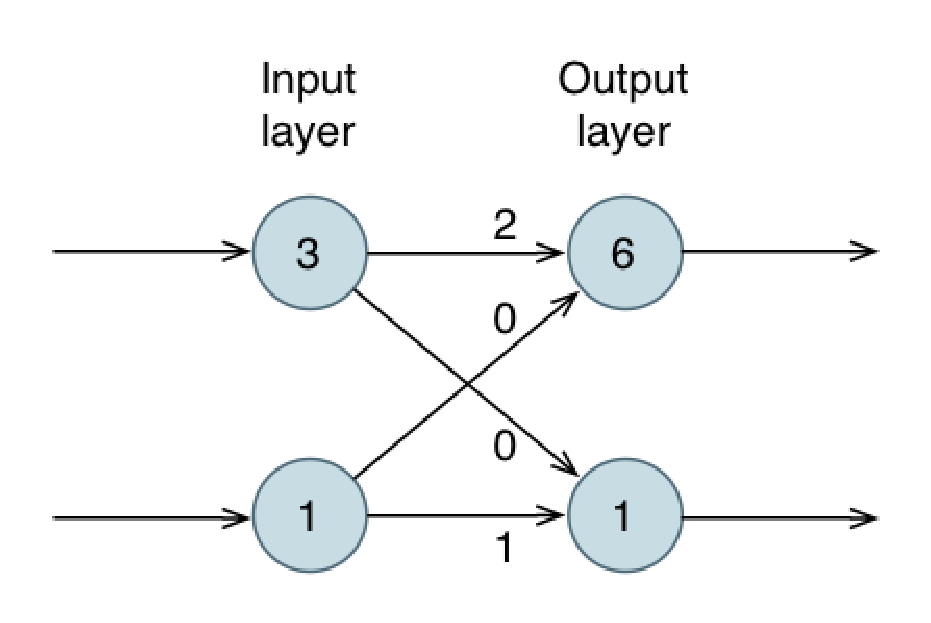
\includegraphics[height=4cm,
    angle=0]{./images/lineartransform_neuralnet.eps},
    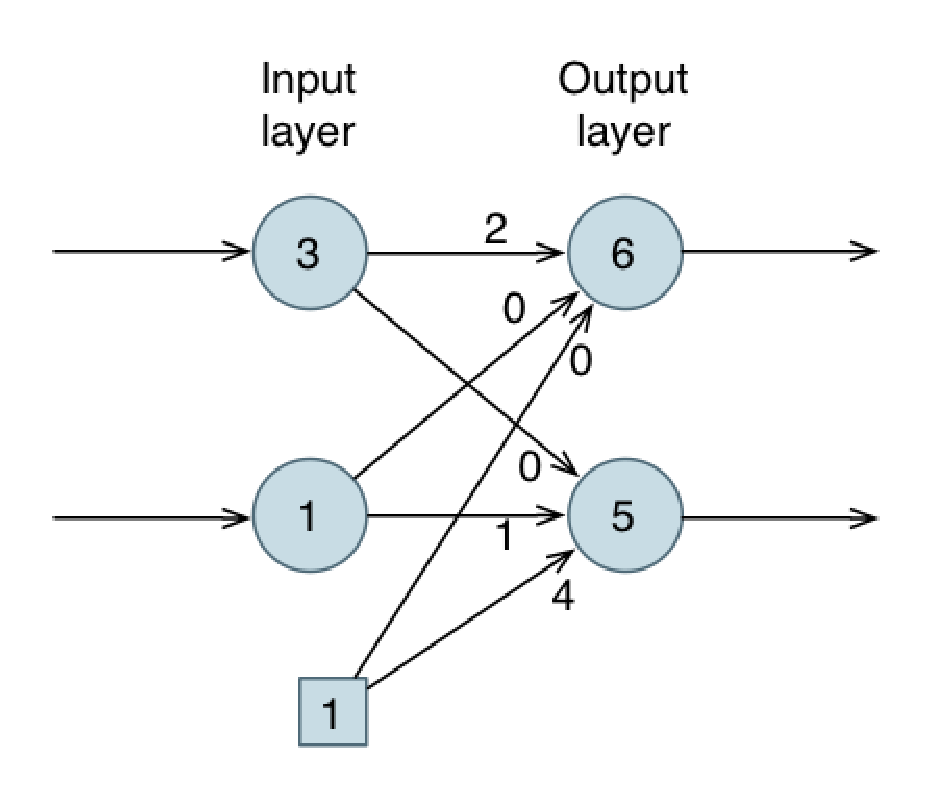
\includegraphics[height=4cm,
    angle=0]{./images/lineartransform_neuralnet_with_bias.eps}}
\caption{(A) Linear transform the neural network way (simple); (B) using Bias vector}
\label{fig:lineartransform_neuralnet}
\end{figure}

In practice, we use affine transformation (Sect.\ref{sec:affine-transformation})
more often in neural network, with $\mathbf{b}$ represents a bias to achieve
some form of {\bf non-linearity}. It means that if the input is zero, we have a
confident that it should belong to a given output class based on the given bias.
Bias vector is also a hyper-parameter.

Consider the bias vector $\mathbf{b} = [0, 4]^T$. Here, the bias is only applied
to the second unit in the output layer, i.e.
the first element of the bias vector is zero; and only the non-zero elements
impose a bias on the output. Using this, we can achieve some form of
non-linearity.

A more real nonlinearity is need to achieve more complicated transformation, and
thus can achieve better learning of a neural network. The idea is that instead
of treating the result of the affine transformation as the output of the node,
we add an additional step, i.e. running the linear combination through a
nonlinear activation function and treating that as the unit output.

There are a whole bunch of different options available for which activation
function you use (Sect.\ref{sec:activation-function-nonlinearity}).

\subsection{sparse matrix}
\label{sec:math-sparse-matrix}

It is common that the matrix $\mathbf{A}$ is sparse, which is to say that it
contains only a small number of non-zero values.

Even if A was a 1 million by 1 million matrix with only 5 million non-zero
entries (and thus we need only store those 5 million), the inverse will
typically have almost every entry non-negative, requiring us to store all 1M -
$\times$ -  1M  entries—that is 1 trillion entries!


There are multiple data structures that can be used to efficiently construct a sparse matrix; three common choices
\begin{enumerate}
  \item  Dictionary of Keys. A dictionary is used where a row and column index is mapped to a value.
  
  \item List of Lists. Each row of the matrix is stored as a list, with each sublist containing the column index and the value.
 
  
  \item Coordinate List. A list of tuples is stored with each tuple containing the row index, column index, and the value.
\end{enumerate}

However, for performing efficient operations, there are different choices of
data structures that are more suitable
\begin{enumerate}
  
  \item Compressed Sparse Row (CSR). The sparse matrix is represented using three
  one-dimensional arrays for the non-zero values, the extents of the rows, and
  the column indexes.
  
 \textcolor{red}{CSR is often used to represent sparse matrices in machine
 learning given the
  efficient access and matrix multiplication that it supports.}
  
  \item Compressed Sparse Column. The same as the Compressed Sparse Row method
  except the column indices are compressed and read first before the row
  indices.
  
\end{enumerate}

In Python, the CSR form of a sparse matrix is created using \verb!scipy.sparse.csr_matrix!
\begin{lstlisting}


# dense to sparse
from numpy import array
from scipy.sparse import csr_matrix
# create dense matrix
A = array([[1, 0, 0, 1, 0, 0], [0, 0, 2, 0, 0, 1], [0, 0, 0, 2, 0, 0]])
print(A)

# convert to sparse matrix (CSR method)
S = csr_matrix(A)
print(S)

# reconstruct dense matrix
B = S.todense()
print(B)


from numpy import count_nonzero

sparsity = 1.0 - count_nonzero(A) / A.size

\end{lstlisting}

The number of non-zero elements in a NumPy array can be given by the \verb!count_nonzero()! function


\subsection{-- in deep learning}


Sparse matrices come up in encoding schemes used in the preparation of data.
\begin{enumerate}
  \item One-hot encoding, used to represent categorical data as sparse binary vectors. 
  
  The output layer with the number of units represent the number of categories, the vector represent one category 
  is a one-hot vector, e.g. one element is zero and all other elements are zeroes. Category-1 is represented by 
  $\mathbf{l} = [1,0,0,\ldots,0]$.
  
  \verb!sklearn.preprocessing.OneHotEncoder! encode categorical features as a one-hot numeric array.
  \url{https://scikit-learn.org/stable/modules/generated/sklearn.preprocessing.OneHotEncoder.html}
  
  \item Count encoding, used to represent the frequency of words in a vocabulary for a document
  
  Suppose there are $n$ words, the vector represent the frequency of all words
  (in a paragraph or a sentence) is represented by $\mathbf{f}= (f_1, f_2,
  \ldots, f_n)$; in that $f_i$ is the frequency of $i$-th word. This is typically a sparse vector.
  
\begin{verbatim}

If there are 100,000 words in the language model, then the feature vector has
length 100,000, but for a short email message almost all the features will have
count zero.
\end{verbatim}

  The minibatch, i.e. a subset of training samples is then represented by a matrix, in that each row is a sparse vector, so 
  the matrix itself is also a sparse matrix.
  
  \verb!sklearn.feature_extraction.text.CountVectorizer! convert a collection of text documents to a matrix of token counts.
  \url{https://scikit-learn.org/stable/modules/generated/sklearn.feature_extraction.text.CountVectorizer.html}
  
  \item TF-IDF encoding, used to represent normalized word frequency scores in a vocabulary.
 
 \verb!sklearn.feature_extraction.text.TfidfVectorizer! convert a collection of raw documents to a matrix of TF-IDF features.
 This is equivalent to CountVectorizer followed by TfidfTransformer.
 
\end{enumerate}

We often need sparse matrix in 
\begin{itemize}	 
  \item  Natural language processing for working with documents of text.
  
  \item Recommender systems for working with product usage within a catalog.
  
  \item Computer vision when working with images that contain lots of black pixels.
\end{itemize}
 
\subsection{Rank of a matrix: linear dependence vs linear independent}
\label{sec:math-matrix-rank}

If we have a general $n-\times-m$ matrix, it is reasonable to ask what dimension
space the matrix maps into.

Some distortions can be severe, e.g. the matrix below compresses the entire
two-dimensional plane down to a single line. This is the example when using a
matrix that has a column is a linear dependence of other columns. In this case,
we call the {\bf rank} of the $n-\times-n$ matrix is lower than $n$.
\begin{equation}
\mathbf{B} = \begin{bmatrix}
2 & -1 \\ 4 & -2
\end{bmatrix},
\end{equation}


\textcolor{red}{A criteria to test of a matrix is of rank} $n$: given the column
vectors are $v_1, \ldots, v_n$; and if there exist coefficients
 $a_1, \ldots, a_n$ not all equal to zero so that
\begin{equation}
\sum_i a_i \mathbf{v}_i = 0
\end{equation}
then the rank must be lower than $n$. 
This procedure, as described, is very inefficient.
It requires looking at every subset of the columns of our given matrix,
and thus is potentially exponential in the number of columns.
\textcolor{red}{Using determinant is a better choice to test the rank} (Sect.\ref{sec:math-matrix-determinant}).

\textcolor{red}{In Python: we use} \verb!numpy.linalg.matrix_rank!, or
\begin{lstlisting}{lang="python"}
def rank(A, eps=1e-12):
    u, s, vh = numpy.linalg.svd(A)
    return len([x for x in s if abs(x) > eps])
\end{lstlisting}

NOTE: \verb!eps! depends in your application - most would agree that 1e-12
corresponds to zero, but you may witness numerical instability even for
\verb!eps=1e-9!.


In particular, the rank of a matrix $\mathbf{A}$ is the largest number of
linearly independent columns amongst all subsets of columns.
The matrix $\mathbf{B}$ above  has \verb!rank(B)! = 1, since the two columns are
linearly dependent, but either column by itself is not linearly dependent.


If a matrix is of rank $n$, i.e. there is no linear dependence, we say the
(column) vectors are linearly independent.

\subsection{Rank vs. SVD}

Suppose a $N\times M$ matrix, and the Singular Value Decomposition (SVD -
Sect.\ref{sec:SVD}) of that matrix $\mathbf{W}$ is
\begin{equation}
\mathbf{W} = \mathbf{U. \Sigma. V^T}
\end{equation}
with $\nu_i = \Sigma_{ii}$ the diagonal element of the matrix $\Sigma$.

The Matrix Rank, or Hard Rank, is simply the number of non-zero singular values
($\nu_i > 0$), i.e. number of non-zero diagonal of the matrix $\Sigma$.

\begin{equation}
\mathcal{R}(\mathbf{W}) = \sum \delta(\nu_i > 0)
\end{equation}

Of course, being a numerical method, we really mean the number of singular
values above some tolerance ($\nu_i > $epsilon) and we can get different results
depending on if we use (either Python default tolerance (epsilon), or numerical recipes
tolerance which is tighter).
\begin{lstlisting}{lang="python"}
def rank(A, eps=1e-12):
    u, s, vh = numpy.linalg.svd(A)
    return len([x for x in s if abs(x) > eps])
\end{lstlisting}



\subsection{Full Rank (=n) vs. Singular matrix (< $n$)}

If all the singular values are non-zero, we say $\mathbf{W}$  is Full Rank. If one
or more $\nu_{i}\sim 0$, then we say $\mathbf{W}$  is Singular.

A Singular matrix has lost expressiveness, and the model has undergone Rank collapse.

\subsection{-- Fixing Rank Collapse: Tikhonov Regularization}

When a model undergoes Rank Collapse, it means multiple input will be mapped to
the same output, i.e. label. This is NOT good.
So, it traditionally needs to be regularized, i.e. we add some small constant
$\gamma$ to the diagonal of the matrix $\mathbf{W}$. This procedure is also
called {\bf Tikhonov Regularization}.  
\begin{equation}
\mathbf{W^T.W} = \mathbf{W^T.W} + \gamma \gamma
\end{equation}

\begin{mdframed}

In cases where $\mathbf{W}$  is Singular, regularization is absolutely necessary.
But even when it is not singular, Regularization can be useful in traditional
machine learning.

\end{mdframed}

So that all the singular values will now be greater than zero, and we can form a
generalized pseudo-inverse, called the {\bf Moore-Penrose Inverse}
(Sect.\ref{sec:Moore-Penrose-inverse}).
\begin{equation}
\mathbf{W}^\dagger = (\mathbf{W^T.W} + \gamma \gamma)^{-1}
\end{equation}

The constant, or Regularizer, $\gamma$ 
sets the Noise Scale for the model.
\begin{enumerate}
  \item {\bf Information}: stays in the singular vector associated with largest singular values $\nu_i > \gamma$
  
  
  \item {\bf Noise}: stays in the singular vector where $\nu_i < \gamma$
\end{enumerate}


\url{https://calculatedcontent.com/2018/09/21/rank-collapse-in-deep-learning/}

\subsection{-- Moore-Penrose Inverse (Generalized Inverse)}
\label{sec:Moore-Penrose-inverse}

Moore-Penrose is the technique for finding the inverse of a rectangular matrix
generalized from square matrix. It is called Moore-Penrose Inverse after two
independent discoverers of the method or the Generalized Inverse.

$m-\times-n$ matrix $\mathbf{A}$. Given \verb!A=V.Sigma.U^T!, the pseudoinverse
is calculated using the singular value decomposition of A:

\begin{verbatim}
A^+ = V . Sigma^+ . U^T
\end{verbatim}

NOTE: U and V can be retrieved from SVD operation. 
For the diagonal matrix, the transpose is the reciprocal of every diagonal elements.
\begin{verbatim}
Sigma^+ = [   1/s11, 0, \ldots 0 
              0     1/s22, \ldots, 0
              \ldots
              0 , \ldots, 1/snn    ]
\end{verbatim}

IMPORTANCE:  The pseudoinverse provides one way of solving the linear regression
equation, specifically when there are more rows than there are columns, which is
often the case.

In Python: NumPy has \verb!pinv()!
\begin{lstlisting}
from numpy.linalg import pinv
# define matrix
A = array([
	[0.1, 0.2],
	[0.3, 0.4],
	[0.5, 0.6],
	[0.7, 0.8]])
print(A)
# calculate pseudoinverse
B = pinv(A)
\end{lstlisting}


\subsection{Rank vs. Determinant}
\label{sec:math-matrix-determinant}

A square matrix is full rank if and only if its determinant is nonzero.

Let $\mathbf{A}$ be an $n-\times-n$ matrix, note that \verb!det(A)! $\ne$ 0 det
\verb!iff! the rows are linearly independent iff \verb!rank(A)=n!.

\begin{lstlisting}{lang="python"}
import numpy as np

mat = np.array([[1, -1], [2, 3]])
np.linalg.det(mat)
\end{lstlisting}

Finding number of non-zero eigenvalues is the rank of a matrix (Sect.\ref{sec:eigendecomposition-usage}).

The determinant can be positive, negative, or zero. 

Computing determinants for larger matrices can be laborious, but the intuition
is the same. The determinant remains the factor that $n-\times-n$ matrices scale
n-dimensional volumes (Sect.\ref{sec:math-linear-transformation}).


\subsection{linear dependence = compress the space}

If the columns of a matrix are linearly independent, no compression occurs and
the operation can be undone.

A linear dependence in the columns of a matrix is a witness to the fact that our
matrix is compressing the space down to some lower dimension.

\subsection{Special matrices: I (identity matrix)}

The {\bf identity matrix} is the matrix with ones along the diagonal, and zeros elsewhere. 
The linear transformation using $\mathbf{I}$ leaves our data unchanged when applied.

This is equivalent to applying to a rank-n matrix $\mathbf{A}$, and then apply
the transformed point to the inverted matrix $\mathbf{A}^{-1}$.

\begin{equation}
\mathbf{A^{-1}  A=AA^{-1} =I.}
\end{equation} 


\subsection{Matrix norm (Frobenius norm)}
\label{sec:math-norm-matrix}


This is equivalent to take the L2 norm of the matrix after flattening, i.e.
turns the matrix into a vector and L2-norm of that vector.

\begin{equation}
||\mathbf{A}||_F = \sqrt{\sum_{i,j}A^2_{i,j}}
\end{equation}


We can use \verb!numpy.linalg.norm(A)!




\section{Hyperplanes}
\label{sec:math-hyperplane}

A hyperplane split the space (of n-dimension) into 2 parts. 

{\bf Hyperplane}, a generalization to higher dimensions of a line (two
dimensions) or of a plane (three dimensions). In an $n$-dimensional vector
space, a hyperplane has $d-1$ dimensions and divides the space into two
half-spaces.


Recall the question we have in Sect.\ref{sec:math-dot-product-vectors}, what are
the points $v$ such that its dot product with a given vector $w$ is 1, i.e.  $w
\cdot v=1$.
Consider $w=[2,1]^T$. \textcolor{red}{IMPORANT: 1 is just a value of choice, and
we call it a threshold}.

The dot product, can be written as 
\begin{equation}
||v|| ||w|| \cos(\theta) = 1
\end{equation}
or
\begin{equation}
||v||  \cos(\theta) = \frac{1}{||w||} = \frac{1}{\sqrt{5}}
\end{equation}

This is equivalent to saying that the length of the projection of $v$ onto the
direction of $w$ is exactly $\frac{1}{||w||}$.

The set of all points where this is true is a line, satisfying the equation
$2x+y=1$.


If we now look at what happens when we ask about the set of points with
\begin{equation}
v \cdot w < 1
\end{equation}
or
\begin{equation}
v \cdot w > 1
\end{equation}
Those two inequalities define either side of the line.

\begin{itemize}
  \item  If, $u$ and $w$ are 3-dimensional vector, then the line becomes a plane. 

  \item If, $u$ and $w$ are n-dimensional vector, then the line becomes a hyperplane of (n-1) dimensions. 
  
\end{itemize}

\subsection{Hyperplane as decision plane}

In ML, where data samples are represented as points (vectors), such hyperplanes
are often referred to as decision planes. 

The majority of deep learned classification models end with a linear layer fed
into a softmax, so one can interpret the role of the deep neural network to be
to find a non-linear embedding such that the target classes can be separated
cleanly by hyperplanes.

\subsection{A crude classifier using hyperplane}
\label{sec:math-hyperplane-threshold}

A classifier, e.g. hyperplane, that can classify tiny images of t-shirts and
trousers from the Fashion MNIST dataset.
\begin{lstlisting}{lang=python}
# Load in the dataset
train = gluon.data.vision.FashionMNIST(train=True)
test = gluon.data.vision.FashionMNIST(train=False)

# each row is a two-element vector, 
#   x[0] = sample
#   x[1] = label
X_train_0 = np.stack([x[0] for x in train if x[1] == 0]).astype(float)
X_train_1 = np.stack([x[0] for x in train if x[1] == 1]).astype(float)

X_test = np.stack(
    [x[0] for x in test if x[1] == 0 or x[1] == 1]).astype(float)
y_test = np.stack(
    [x[1] for x in test if x[1] == 0 or x[1] == 1]).astype(float)

\end{lstlisting}
In Python: \verb!numpy.stack()! function is used to join a sequence of same
dimension arrays along a new axis. By default, \verb!iterator! iterates by row. 

The mean point in each group is calculated, $u$ and $w$ respectively. The two
points form a vector, $v=u-w$.
\begin{lstlisting}{lang=python}
# Compute averages
ave_0 = np.mean(X_train_0, axis=0)
ave_1 = np.mean(X_train_1, axis=0)


# Plot average t-shirt
d2l.set_figsize()
d2l.plt.imshow(ave_0.reshape(28, 28).tolist(), cmap='Greys')
d2l.plt.show()

# Plot average trousers 
d2l.plt.imshow(ave_1.reshape(28, 28).tolist(),
cmap='Greys') d2l.plt.show()
\end{lstlisting}
The mean point itself is also an image. In this case, when we plot the two mean
points, they shows two blurry images of a t-shirt, and a trousers.

Here, taking the vector between their means to define the decision plane and
eyeball a crude threshold The average is itself an image, which in this case
indeed resembles a blurry image of a t-shirt.
 
Using the mean points, the difference forms a row vector, $v=u-w$; so we take
the transform to get a column vector
\begin{lstlisting}{lang=python}
# Print test set accuracy with eyeballed threshold
w = (ave_1 - ave_0).T
\end{lstlisting}

Now, we find a hyperplane that is best at splitting the points in each group.
The choice of this hyperplane is given by the choice of the threshold value
$t=-1500000$.

Example: 
\begin{lstlisting}{lang=python}
predictions = X_test.reshape(2000, -1).dot(w.flatten()) > -1500000

# Accuracy
np.mean(predictions.astype(y_test.dtype) == y_test, dtype=np.float64)
\end{lstlisting}


\subsection{SVM}
\label{sec:math-hyperplane-SVM}

Support Vector Machine (SVM) provides a strategy for finding the right
hyperplane. The plane is chosen based on the choices of a number of points
called {\bf support vectors}.


Support Vector Machine is a linear model for classification and regression
problems. It can solve linear and non-linear problems and work well for many
practical problems. The idea of SVM is simple: The algorithm creates a line or a
hyperplane which separates the data into classes.
 
 
\section{Tensor}
\label{sec:tensor}

We have worked with vector, matrix.
Rather treating each differently, a unified view on a number of matrix and
vector operations is provided via {\bf tensor}. 

In matrix multiplication, $\mathbf{C = A B}$, the formula to find elements of $\mathbf{C}$ is
\begin{equation}
c_{i, j} = \sum_{k} a_{i, k}b_{k, j}.
\end{equation}

With tensor, a generalized formula is used, in that user needs to specify the coefficients
\begin{equation}
y_{il} = \sum_{jk} x_{ijkl}a_{jk}.
\end{equation}
Such a transformation is called a {\bf tensor contraction.}
This represents a far more flexible family of transformations
that matrix multiplication alone.

\begin{mdframed}
Simplified math notation: Einstein notation,
where the summation is implicitly taken over all repeated indices.

\begin{equation}
y_{il} = x_{ijkl}a_{jk}.
\end{equation}
\end{mdframed}

{\bf Tensor notations}:
\begin{enumerate}
  \item  $\mathbf{v} \cdot \mathbf{w} = \sum_i v_iw_i$
\item  $\|\mathbf{v}\|_2^{2} = \sum_i v_iv_i$
\item  $(\mathbf{A}\mathbf{v})_i = \sum_j a_{ij}v_j$
\item  $(\mathbf{A}\mathbf{B})_{ik} = \sum_j a_{ij}b_{jk}$
\item  $\mathrm{tr}(\mathbf{A}) = \sum_i a_{ii}$
\end{enumerate}

In Python
\begin{lstlisting}{lang="python"}
# Define tensors
B = np.array([[[1, 2, 3], [4, 5, 6]], [[7, 8, 9], [10, 11, 12]]])
A = np.array([[1, 2], [3, 4]])
v = np.array([1, 2])

# Print out the shapes
A.shape, B.shape, v.shape
\end{lstlisting}




\chapter{Eigendecomposition: eigenvalue + eigenvector}
\label{sec:eigendecomposition}

We have learnt {\bf matrix } (Sect.\ref{sec:math-matrix}), and linear transformation (Sect.\ref{sec:math-linear-transformation}).

Matrix decomposition, also known as matrix factorization, involves describing a given matrix using its constituent elements.
\begin{enumerate}

  \item Eigendecomposition refers to a technique that we rewrite the given matrix in its
new form (Sect.\ref{sec:decomposition-matrix}) using eigenvalues and
eigenvectors.
  
  \item  SVD is a matrix decomposition technique (Sect.\ref{sec:SVD}).

All matrices have an SVD, which makes it more stable than other methods, such as
the eigendecomposition.

\end{enumerate}



Suppose matrix $\mathbf{A}$
\begin{equation}
\mathbf{A} = \begin{bmatrix}
2 & 0 \\
0 & -1
\end{bmatrix}.
\end{equation}

which transforms a vector $\mathbf{v} = [x, y]^\top$ to a new one $\mathbf{v}A =
[2x, -y]^\top$.

Typically, this transformation is applied to every dimension.
Namely $[1, 0]^\top$ gets sent to $[2, 0]^\top$ and $[0, 1]^\top$ gets sent to
$[0, -1]^\top$.  An intuitive interpretation is that the transformation stretch
the vector to be twice as wide in the $x$-direction, and then flip it in the
$y$-direction.


However, there are some vectors for which something remains unchanged, i.e. it
changes homogeneously to every element (or geometrically, it does not change the
direction of the vector). The transformed vectors are still in the same line of
the origin vectors. \textcolor{red}{This is an interesting property} as we will
discover here.


If  $\mathbf{A}$ is fixed, in general, we can find a number 
$\lambda$ and a vector 
$\mathbf{v}$  such that
\begin{equation}
\mathbf{A. v} = \lambda \mathbf{v}
\end{equation}
It means that matrix $\mathbf{A}$ applied to the vector $\mathbf{v}$ only scale the vector with a
coefficient $\lambda$. In Python it means \verb!dot(a,v) = w * v!

In the above example, $\lambda = 2$ when $\mathbf{v} = [1,0]^\top$.

We say that $\mathbf{v}$ is an eigenvector and $\lambda$ is an
eigenvalue for matrix $\mathbf{A}$.

\section{Eigenvalue: how to find}

REMEMBER: using the fact that the eigenvalues of a diagonal matrix are its
diagonal elements. 
Efficient, accurate methods to compute eigenvalues and eigenvectors of arbitrary
matrices were not known until the QR algorithm was designed in 1961.

We solve the equation
\begin{equation}
(\mathbf{A} - \lambda \mathbf{I})\mathbf{v} = 0
\end{equation}

We see that  $\mathbf{A- \lambda I)}$
must compress some direction down to zero,
hence it is not invertible, and thus the determinant is zero.

Thus, we can find the *eigenvalues* by finding for what $\lambda$ is
$\det(\mathbf{A}-\lambda \mathbf{I}) = 0$. This is discussed in
Sect.\ref{sec:math-matrix-determinant}.
Solving this polynomial equation returns all values of $\lambda$.


Python provides the code
\begin{enumerate}
  
  \item   \verb!numpy.linalg.eigvals()! method; or \verb!scipy.linalg.eigvals()!
  
  based on \verb!_geev! LAPACK routines which compute the eigenvalues and eigenvectors of general square arrays.
  
  \item or \verb!numpy.linalg.eig()!: return eigenvalue (w), and eigenvector (v); 
  or \verb!scipy.linalg.eig()!
  
  also based on \verb!_geev! LAPACK.
  
  NOTE: SciPy contains more fully-featured versions of the linear algebra
  modules, as well as many other numerical algorithms.
  
\end{enumerate}


\begin{lstlisting}{lang="python"}
%matplotlib inline
import d2l
from IPython import display
import numpy as np
from numpy import linalg as LA

w, v = LA.eig(np.array([[2, 1], [2, 3]]))

w = np.linalg.eigvals(np.array([[2, 1], [2, 3]]))


# Compute the eigenvalues
eigs = np.linalg.eigvals(A).tolist()
\end{lstlisting}

NOTE: Note that numpy normalizes the eigenvectors to be of length one,
whereas we took ours to be of arbitrary length.
Additionally, the choice of sign is arbitrary.

Eigenvalues are often difficult to reason with intuitively.
If presented an arbitrary matrix, there is little that can be said about what
the eigenvalues are without computing them. There are a number of theorems that
can provide some insights without computing them.
\begin{enumerate}
  \item Gershgorin Circle Theorem (Sect.\ref{sec:Gershgorin-Circle-Theorem})
\end{enumerate}

The largest eigenvalue of a matrix is aka {\bf principle eigenvalue} (Sect.\ref{sec:principle-eigenvalue}).

\subsection{Gershgorin Circle Theorem}
\label{sec:Gershgorin-Circle-Theorem}

If the exact value of eigenvalues are not important, i.e. an approximated value
is good enough, we can avoid the expensive computation to calculate the
eigenvalues. The {\bf Gershgorin Circle Theorem} can provide approximate values for
the eigenvalues of a matrix.



Let $\mathbf{A} = (a_{ij})$ be any square matrix ($n\times n$).
We will define $r_i = \sum_{j \neq i} |a_{ij}|$.
Let $\mathcal{D}_i$ represent the disc in the complex plane 
with center $a_{ii}$ radius $r_i$.
Then, every eigenvalue of $\mathbf{A}$ is contained in one of the $\mathcal{D}_i$.


Example to explain the theorem: Consider this matrix

\begin{equation}
\mathbf{A} = \begin{bmatrix}
1.0 & 0.1 & 0.1 & 0.1 \\
0.1 & 3.0 & 0.2 & 0.3 \\
0.1 & 0.2 & 5.0 & 0.5 \\
0.1 & 0.3 & 0.5 & 9.0
\end{bmatrix}.
\end{equation}

The four radius are:  $r_1 = 0.3$, $r_2 = 0.6$, $r_3 = 0.8$ and $r_4 = 0.9$.

This means that all of our eigenvalues will be in one of the ranges of 

$$[a_{11}-r_1, a_{11}+r_1] = [0.7, 1.3], $$

$$[a_{22}-r_2, a_{22}+r_2] = [2.4, 3.6], $$

$$[a_{33}-r_3, a_{33}+r_3] = [4.2, 5.8], $$

$$[a_{44}-r_4, a_{44}+r_4] = [8.1, 9.9]. $$


To double check, we compute the four eigenvalues
\begin{lstlisting}
A = np.array([[1.0, 0.1, 0.1, 0.1],
              [0.1, 3.0, 0.2, 0.3],
              [0.1, 0.2, 5.0, 0.5],
              [0.1, 0.3, 0.5, 9.0]])

v, _ = np.linalg.eig(A) 
v
\end{lstlisting}

The eigenvalues are approximately 0.99, 2.97, 4.95, 9.08, all comfortably inside
the ranges provided.


\textcolor{red}{\bf What does it means?} If the diagonal $a_{ii}$ is
significantly larger than all the other elements, it means the range will be
small; which enables the approximations of eigenvalues will be fairly accurate.





\section{Eigenvector: how to find}

Eigenvectors are vectors which are stretched by a matrix without changing
direction. Eigenvalues are the amount that the eigenvectors are stretched by the
application of the matrix. 

Once we find the eigenvalues, we can solve 
$\mathbf{A}\mathbf{v} = \lambda \mathbf{v}$ 
to find the associated *eigenvector(s)*.

All the eigenvetors can be written as column vectors of a matrix
\begin{equation}
\mathbf{W} = \begin{bmatrix}
1 & 1 \\
-1 & 2
\end{bmatrix},
\end{equation}
be the matrix where the columns are the eigenvectors of the matrix $\mathbf{A}$.

Efficient, accurate methods to compute eigenvalues and eigenvectors of arbitrary
matrices were not known until the QR algorithm was designed in 1961. Combining
the Householder transformation with the LU decomposition results in an algorithm
with better convergence than the QR algorithm.


It is not always possible to find enough linearly independent eigenvectors. To
handle such matrices, we require more advanced techniques than we can cover
(such as the Jordan Normal Form, or Singular Value Decomposition).

\subsection{Jordan Normal Form}

Jordan Normal Norm is an advanced technique to find eigenvalues and eigenvectors.


\section{Singular Value Decomposition (SVD)}
\label{sec:SVD}


All matrices have an SVD, which makes it more stable than other methods, such as the eigendecomposition.

With SVD, it turns a matrix into other matrices such that it makes certain
subsequent matrix calculations simpler.
\begin{lstlisting}
A = U . Sigma . V^T
\end{lstlisting}
\begin{itemize}
  \item A : $m-\times-n$ real matrix
  
  \item U: $m-\times-m$ matrix
 
 The columns of the U matrix are called the left-singular vectors of A
  
  \item Sigma: $m-\times-n$ diagonal matrix
  
  The diagonal values in the Sigma matrix are known as the singular values of the original matrix A. 
  
  \item $V^T$: the  transpose of an n x n matrix 

 The columns of V are called the right-singular vectors of A.
 
\end{itemize}

The SVD is calculated via iterative numerical methods.

\begin{mdframed}

Every rectangular matrix has a singular value decomposition, although the
resulting matrices may contain complex numbers and the limitations of floating
point arithmetic may cause some matrices to fail to decompose neatly.

The SVD allows us to discover some of the same kind of information as the
eigendecomposition. However, the SVD is more generally applicable.

The SVD is used widely both in the calculation of other matrix operations, such
as matrix inverse, but also as a data reduction method in machine learning. SVD
can also be used in least squares linear regression, image compression, and
denoising data.

\end{mdframed}

In Python
\begin{lstlisting}
from numpy import array
from scipy.linalg import svd

A = array([[1, 2], [3, 4], [5, 6]])

# SVD
U, s, VT = svd(A)
\end{lstlisting}

IMPORTANT: The U, s, and V elements returned from the svd() cannot be multiplied directly.
\begin{itemize}
  \item  The s vector must be converted into a diagonal matrix using the diag() function.
  
  By default, it creates a square matrix that is n x n, relative to our original matrix.
  However, what we need is a $m-\times-n$ matrix. 
  
  We can achieve this by creating a new Sigma matrix of all zero values that is
  m x n (e.g. more rows) and populate the first n x n part of the matrix with
  the square diagonal matrix calculated via diag().
\begin{lstlisting}
from numpy import diag

# create m x n Sigma matrix
Sigma = zeros((A.shape[0], A.shape[1]))
# populate Sigma with n x n diagonal matrix
Sigma[:A.shape[1], :A.shape[1]] = diag(s)
\end{lstlisting}
  
  \item Reconstruct the matrix
\begin{verbatim}
from numpy import dot

# reconstruct matrix
B = U.dot(Sigma.dot(VT))
\end{verbatim}
\end{itemize}

\section{Eigendecomposition: matrix decomposition into eigenvalues + eigenvectors}
\label{sec:decomposition-matrix}

The eigenvalues can also be written in matrix form, i.e. a diagonal matrix in that eigenvalues resides on the diagonal line.
\begin{equation}
\boldsymbol{\Sigma} = \begin{bmatrix}
1 & 0 \\
0 & 4
\end{bmatrix},
\end{equation}
be the matrix with the associated eigenvalues on the diagonal.

Then, collectively, we can write in matrix form 
\begin{equation}
\mathbf{A}\mathbf{W} =\mathbf{W} \boldsymbol{\Sigma} .
\end{equation}


The matrix $W$ is invertible, so we may multiply both sides by $W^{-1}$ on the right,
\begin{equation}
\mathbf{A} = \mathbf{W} \boldsymbol{\Sigma} \mathbf{W}^{-1}.
\end{equation}

Such a decomposition of matrix $\mathbf{A}$ will exist as long as we can find a
full collection of linearly independent eigenvectors (so that W is
invertible). We will learn there are nice consequences of this (Sect.\ref{sec:eigendecomposition-usage}).

\subsection{Symmetric matrix}


The most commonly encountered family are the *symmetric matrices*,
which are those matrices where $\mathbf{A} = \mathbf{A}^\top$. 

We may take $W$ to be an *orthogonal matrix*—a matrix whose columns are all
length one vectors that are at right angles to one another, where
$\mathbf{W}^\top = \mathbf{W}^{-1}$—and all the eigenvalues will be real.

\begin{equation}
\mathbf{A} = \mathbf{W}\boldsymbol{\Sigma}\mathbf{W}^\top .
\end{equation}




\section{The importance of eigendecomposition}
\label{sec:eigendecomposition-usage}

Eigendecompositions can simplify many linear-algebraic computations
and are a fundamental operation underlying many numerical algorithms
and much of the analysis that we do in linear algebra.

The eigendecomposition of a matrix can allow for many operations to be reduced
to operations on the eigenvalues.

We can 
\begin{enumerate}
  \item compute the positive power of a matrix just by raing the eigenvalues to the same power.
  
\begin{equation}
\mathbf{A}^n = \overbrace{\mathbf{A}\cdots \mathbf{A}}^{\text{$n$ times}} = \overbrace{(\mathbf{W}\boldsymbol{\Sigma} \mathbf{W}^{-1})\cdots(\mathbf{W}\boldsymbol{\Sigma} \mathbf{W}^{-1})}^{\text{$n$ times}} =  \mathbf{W}\overbrace{\boldsymbol{\Sigma}\cdots\boldsymbol{\Sigma}}^{\text{$n$ times}}\mathbf{W}^{-1} = \mathbf{W}\boldsymbol{\Sigma}^n \mathbf{W}^{-1}.
\end{equation}
  
  For any positive power of a matrix, the eigendecomposition is obtained by just raising the eigenvalues to the same power.

  \item invert the matrix just by inverting the eigenvalues

\begin{equation}
\mathbf{A}^{-1} = \mathbf{W}\boldsymbol{\Sigma}^{-1} \mathbf{W}^{-1},
\end{equation}

This will work as long as each eigenvalue is non-zero, so we see that invertible
is the same as having no zero eigenvalues.

  \item quickly compute the determinant of a matrix (Sect.\ref{sec:math-matrix-determinant}) 

If $\lambda_1, \ldots, \lambda_n$ 
are the eigenvalues of a matrix, then the determinant of that matrix is
\begin{equation}
\det(\mathbf{A}) = \lambda_1 \cdots \lambda_n,
\end{equation}

This makes sense intuitively because whatever stretching $\mathbf{W}$ does,
$W^{-1}$ undoes it, so in the end the only stretching that happens is by
multiplication by the diagonal matrix $\boldsymbol{\Sigma}$, which stretches
volumes by the product of the diagonal elements.

  \item compute the rank (Sect.\ref{sec:math-matrix-rank}) which is the same as
  the number of non-zero eigenvalues of $\mathbf{A}$.

\end{enumerate}

\section{Eigenvalues/Eigenvectors in traditional ML}


In linear methods from unsupervised learning (e.g. factor analysis also known as
Principal Component Analysis) and supervised learning (e.g. discriminant
analysis) eigenvectors are used.

In factor analysis (Principal Component Analysis, PCA), we take the Covariance
matrix and we try to represent our data set in a new coordinate system that is
transformed.

Imagine you have images (which are high dimensional) as inputs. The goal is to
find a new coordinate system which captures a maximal amount of variance in the
images.

\url{https://math.stackexchange.com/questions/3153522/why-are-eigenvectors-important-for-deep-learning-applications}


\section{Eigenvalues/Eigenvectors in Deep Learning}
\label{sec:deep-learing-mathematical-intuition-init-weights}

Eigenvectors are not so important in deep learning. Deep learning is using
highly nonlinear transformations. That is why concepts from linear algebra like
eigenvalues and eigenvectors do not play a major role in this field.

There might be other fields in machine learning where eigenvalues and
eigenvectors are important. But the core of deep learning relies on nonlinear
transformations. Eigenvalues and eigenvectors are a core concept from linear
algebra but not for the description of nonlinear transformations.
 

\textcolor{red}{In deep neural net, we will see that mathematically, an input
vector is mapped to the output by interspersing layers
of linear transformations with non-linear operations.}

In the simple scenario, we consider only linear transformation, i.e.
a series of matrix multiplication.
\begin{equation}
\mathbf{v}_{out} = \mathbf{A_1}\cdot \mathbf{A_k}\cdots \mathbf{A_n} \mathbf{v}_{in}
\end{equation}

\textcolor{red}{REMEMBER}: The learning process is the one that adjust weights,
or elements of the matrices $\mathbf{A}_k$.

In the simplest case, for a toy model, the transformation is a single repeated matrix operation 
$\mathbf{A}$
\begin{equation}
\mathbf{v}_{out} = \mathbf{A}\cdot \mathbf{A}\cdots \mathbf{A} \mathbf{v}_{in} = \mathbf{A}^N \mathbf{v}_{in}.
\end{equation}

For simplicity in our toy model, we will assume that the data vector we feed in
$\mathbf{v}_{in}$ is a random five dimensional Gaussian vector.

\textcolor{red}{Now, the question is how we initialize values of} $\mathbf{A}$? 
A common choice is that $\mathbf{A}$ is taken to be a random matrix
with Gaussian entries.

\begin{lstlisting}{lang="python"}
np.random.seed(8675309)

k = 5
A = np.random.randn(k, k)
A
\end{lstlisting}

\textcolor{red}{The more important question is whether exist a first principle
for making the choice of initial values of } $\mathbf{A}$? Does it always result
a similar  training performance?



\subsection{The tricky part? - stretching}

For context, lets think of a generic ML problem, where we are trying to turn
input data, like an image, into a prediction, like the probability the image is
a picture of a cat.

If repeated application of $\mathbf{A}$ stretches a random vector out to be very long,
then small changes in input will be amplified into large changes in output—tiny
modifications of the input image would lead to vastly different predictions.
This does not seem right!

Example: The norm is growing uncontrollably!
\begin{lstlisting}{lang="python"}
# Calculate the sequence of norms after repeatedly applying A
v_in = np.random.randn(k, 1)

norm_list = [np.linalg.norm(v_in)]
for i in range(1, 100):
    v_in = A.dot(v_in)
    norm_list.append(np.linalg.norm(v_in))

d2l.plot(np.arange(0, 100), norm_list, 'Iteration', 'Value')
\end{lstlisting}

\subsection{The tricky part? - shrinking}

On the flip side, if $\mathbf{A}$ shrinks random vectors to be shorter, then after
running through many layers, the vector will essentially shrink to nothing, and
the output will not depend on the input. This is also clearly not right either!

\subsection{The hint in the increasing of the vector norm?}

After each matrix multiplication, we calculate the norm of the new output vector of each layer. If we take the ratio, 
and see how the norms change. 

\begin{mdframed}

\begin{lstlisting}{lang="python"}
# Compute the scaling factor of the norms
norm_ratio_list = []
for i in range(1, 100):
    norm_ratio_list.append(norm_list[i]/norm_list[i - 1])

d2l.plot(np.arange(1, 100), norm_ratio_list, 'Iteration', 'Ratio')
\end{lstlisting}

If we look at the last portion of the above computation, we see that the random
vector is stretched by a factor of 1.974459321485[...], where the portion at
the end shifts a little, but the stretching factor is stable.

\end{mdframed}


REMEMBER: We have seen that eigenvectors and eigenvalues correspond to the
amount something is stretched, but that was for specific vectors, and specific
stretches.

Now, find the eigenvalues and eigenvectors of this matrix $\mathbf{A}$.
A bit of a caveat here: it turns out that to see them all, we will need to go to
complex numbers which you can think of these as stretches and rotations.
By taking the norm of the complex number (square root of the sums of squares of
real and imaginary parts), we can measure that stretching factor.

\begin{lstlisting}{lang="python"}
# Compute the eigenvalues
eigs = np.linalg.eigvals(A).tolist()
norm_eigs = [np.absolute(x) for x in eigs]
norm_eigs.sort()
"Norms of eigenvalues: {}".format(norm_eigs)
\end{lstlisting}

\textcolor{red}{Huraaaaah}: The number we identified before for the long term
stretching of our matrix $\mathbf{A}$ applied to a random vector is *exactly*
(accurate to thirteen decimal places!) the largest eigenvalue of $\mathbf{A}$.
This is clearly not a coincidence!


This is so important that the largest eigenvalue/eigenvector is called the
*principle eigenvalue* and *principle eigenvector*.


\subsection{Input vector turned into principle eigenvector: power iteration technique}
\label{sec:principle-eigenvalue}

Consider a random vector.
This random vector points a little in every direction, so in particular, it
points at least a little bit in the same direction as the eigenvector of
$\mathbf{A}$ associated with the largest eigenvalue (aka the {\bf principle
eigenvalue}).

After applying $\mathbf{A}$, our random vector gets stretched in every possible
direction, as is associated with every possible eigenvector, but it is stretched
most of all in the direction associated with this principle eigenvector.

What this means is that after apply in $A$, our random vector is longer, and
points in a direction closer to being aligned with the principle eigenvector.

After applying the matrix many times, the alignment with the principle
eigenvector becomes closer and closer until, for all practical purposes, our
random vector has been transformed into the principle eigenvector!

\begin{mdframed}

Indeed this algorithm is the basis for what is known as the *power iteration*
for finding the largest eigenvalue and eigenvector of a matrix (Van-Loan.Golub.1983).

\end{mdframed}

\subsection{Matrix initialization in Deep Net w.r.t principle eigenvalues}
\label{sec:matrix-initialization}

The relationship between the eigenvalues (and a related object called singular
values) of random matrices has been shown to have deep connections to proper
initialization of neural networks (Pennington.Schoenholz.Ganguli.2017).

\subsection{-- Normalization matrix: principle eigenvalue = 1}
\label{sec:normalization-eigenvalue}

So, to prevent the stretching from happening, one good way is to make the {\bf principle eigenvalue} become one.
If we rescale our matrix by this principle eigenvalue so that the largest
eigenvalue is instead now just one.

\begin{lstlisting}{lang="python"}
# Rescale the matrix A
A /= norm_eigs[-1]

# Do the same experiment again
v_in = np.random.randn(k, 1)

norm_list = [np.linalg.norm(v_in)]
for i in range(1, 100):
    v_in = A.dot(v_in)
    norm_list.append(np.linalg.norm(v_in))

d2l.plot(np.arange(0, 100), norm_list, 'Iteration', 'Value')
\end{lstlisting}

So, by normalizing the matrix by its largest eigenvalue, we now can walk the
narrow line between growth and decay to make sure that our output changes
depending on our input, but not much!

Check again the ratio of vector norms
\begin{lstlisting}{lang="python"}
# Also plot the ratio
norm_ratio_list = []
for i in range(1, 100):
    norm_ratio_list.append(norm_list[i]/norm_list[i-1])

d2l.plot(np.arange(1, 100), norm_ratio_list, 'Iteration', 'Ratio')
\end{lstlisting}


After normalizing the matrices by the principle eigenvalue, we see that the
random data does not explode as before, but rather eventually equilibrates to a
specific value.

\textcolor{red}{How can we estimate this principle eigenvalue?}


\subsection{Estimate principle eigenvalue}

The largest eigenvalue of a large random $n-\times-n$ matrix with independent mean zero,
variance one Gaussian entries is on average about $\sqrt{n}$.

In the above examples, $\mathbf{A} = np.rand(5, 5)$, its largest eigenvalue is
about $\sqrt{5} = 2.2$.

This is thanks to the fascinating fact known as the {\bf circular law}
(Ginibre.1965).


\chapter{Calculus: derivative}


\section{Learning matrix's weights}
\label{sec:learning-matrix-weights}
\label{sec:deep-learing-mathematical-intuition-learn-weights}

In Sect.\ref{sec:deep-learing-mathematical-intuition-init-weights},
we have talked about the important of matrix initialization by normalizing that
matrix using principle eigenvalue (Sect.\ref{sec:matrix-initialization}). Let's
talk about learning the weights.

Suppose that we have a deep neural network where the weights (from multiple
matrices across all layers) are, for convenience, concatenated into a single
vector $\mathbf{w} = (w_1, \ldots,w_n)$.

Given a training dataset, the series of matrix transformation (across multiple
layers) produce a final output vector $\mathbf{v}_{out}$.
This vector can be different from the expected output, which we consider the
loss of our neural network on this dataset, and is written as
$\mathcal{L}(\mathbf{w})$.

This loss function is extraordinarily complex, encoding the performance of all
possible models of the given architecture on this dataset, so it is nearly
impossible to tell what set of weights $\mathbf{w}$ will minimize the loss.

The most important question is how do we find the direction which makes the
weights decrease as quickly as possible? - The mathematical tool is {\bf
differential calculus}. \textcolor{red}{Differential calculus is fundamentally
the study of how functions behave under small changes. This is the core of deep
learning.}

In practice, we often start by initializing our weights {\it randomly}, and then
iteratively take small steps in the direction which makes the loss decrease as
rapidly as possible.

Let's start with the case with weght is a single variable
(Sect.\ref{sec:single-value-differential-calculus}). Then, we extend that to a
weight vector using multivariable calculus
(Sect.\ref{sec:multivariable-differential-calculus}).
Finally, we explain how the weights should be changed in the so-called 
{\bf direction of steepest descent} (Sect.\ref{sec:deep-learing-mathematical-intuition-learn-weights-steepest-descent-direction})


\section{Single-value differential calculus}
\label{sec:single-value-differential-calculus}


Let's first examine the case with only a single weight: $L(\mathbf{w}) = L(x)$
for a single real value $x$.

Let's take $x$ and try to understand what happens when we change it by a small
amount to $x + \epsilon$.

The function $f(x) = sin(x^x)$, over the range [0, 3]
\begin{lstlisting}{lang="python"}
%matplotlib inline
import d2l
from IPython import display
from mxnet import np, npx
npx.set_np()

# Plot a function in a normal range
x_big = np.arange(0.01, 3.01, 0.01)
ys = np.sin(x_big**x_big)
d2l.plot(x_big, ys, 'x', 'f(x)')
\end{lstlisting}
The shape of the function is too complicated. 

A simpler form if we reduce the range to [1.75, 2.25]
\begin{lstlisting}
# Plot a the same function in a tiny range
x_med = np.arange(1.75, 2.25, 0.001)
ys = np.sin(x_med**x_med)
d2l.plot(x_med, ys, 'x', 'f(x)')
\end{lstlisting}

And it is even simpler if we zoom in a tiny range
\begin{lstlisting}
# Plot a the same function in a tiny range
x_small = np.arange(2.0, 2.01, 0.0001)
ys = np.sin(x_small**x_small)
d2l.plot(x_small, ys, 'x', 'f(x)')
\end{lstlisting}

If we make the range small enough, it looks like a straight line.
This is the key observation of single variable calculus: the behavior of
familiar functions can be modeled by a line in a small enough range.

Assuming the tiny change $\varepsilon$ is small enough, an appriximation for the new value is
\begin{equation}
\frac{L(x+\epsilon) - L(x)}{(x+\epsilon) - x} = \frac{L(x+\epsilon) - L(x)}{\epsilon}.
\end{equation}

\begin{lstlisting}
# Define our function
def L(x):
    return x**2 + 1701*(x-4)**3

# Print the difference divided by epsilon for several epsilon
for epsilon in [0.1, 0.001, 0.0001, 0.00001]:
    print("epsilon = {:.5f} -> {:.5f}".format(
        epsilon, (L(4+epsilon) - L(4)) / epsilon))
\end{lstlisting}


\subsection{Common derivatives}

\begin{enumerate}

\item Derivative of constants.** $\frac{d}{dx}c = 0$.
\item Derivative of linear functions.** $\frac{d}{dx}(ax) = a$.
\item Power rule.** $\frac{d}{dx}x^n = nx^{n-1}$.
\item Derivative of exponentials.** $\frac{d}{dx}e^x = e^x$.
\item Derivative of the logarithm.** $\frac{d}{dx}\log(x) = \frac{1}{x}$.
\end{enumerate}

\subsection{Derivative rules}

We needs rules to compute the derivative of more complex function, using simpler function

\begin{enumerate}

\item Sum rule.** $\frac{d}{dx}\left(g(x) + h(x)\right) = \frac{dg}{dx}(x) + \frac{dh}{dx}(x)$.
\item Product rule.** $\frac{d}{dx}\left(g(x)\cdot h(x)\right) = g(x)\frac{dh}{dx}(x) + \frac{dg}{dx}(x)h(x)$.
\item Chain rule.** $\frac{d}{dx}g(h(x)) = \frac{dg}{dh}(h(x))\cdot \frac{dh}{dx}(x)$.
\end{enumerate}

Any function we can write down using sums, products, constants, powers,
exponentials, and logarithms can have its derivate computed mechanically by
following these rules. This is the topics of {\bf Taylor series expansion}


\subsection{-- Meaning of derivatives}

Take a function $f$ and compute the derivative $\frac{df}{dx}$.  This gives us
the rate of change of $f$ at any point.



\subsection{--Taylor series expansion}

The *Taylor series* provides a method to approximate the function $f(x)$ if we
are given values for the first $n$ derivatives at a point $x_0$, i.e., $\left\{
f(x_0), f^{(1)}(x_0), f^{(2)}(x_0), \ldots, f^{(n)}(x_0) \right\}$. The idea
will be to find a degree $n$ polynomial that matches all the given derivatives
at $x_0$.

\begin{lstlisting}
# Compute the exponential function
xs = np.arange(0, 3, 0.01)
ys = np.exp(xs)

# Compute a few Taylor series approximations
P1 = 1 + xs
P2 = 1 + xs + xs**2 / 2
P5 = 1 + xs + xs**2 / 2 + xs**3 / 6 + xs**4 / 24 + xs**5 / 120

d2l.plot(xs, [ys, P1, P2, P5], 'x', 'f(x)', legend=[
    "Exponential", "Degree 1 Taylor Series", "Degree 2 Taylor Series",
    "Degree 5 Taylor Series"])
\end{lstlisting}

\subsection{Second-order derivatives}


However, the derivative, $\frac{df}{dx}$, can be viewed as a function itself, so
nothing stops us from computing the derivative of $\frac{df}{dx}$ to get
$\frac{d^2f}{dx^2} = \frac{df}{dx}\left(\frac{df}{dx}\right)$.  We will call
this the second derivative of $f$.  This function is the rate of change of the
rate of change of $f$, or in other words, how the rate of change is changing.

\begin{enumerate}
  \item   {\bf Positive} value: 
  
  When the second derivative $f^{(2)}(x)$ is a positive constant.  This means
  that the slope of the first derivative is positive.  As a result, the first
  derivative $f^{(1)}(x)$ may start out negative, becomes zero at a point, and
  then becomes positive in the end. This tells us the slope of our original
  function $f$ and therefore, the function $f$ itself decreases, flattens out,
  then increases.  In other words, the function $f$ curves up, and has a single
  minimum
  
  \item {\bf Negative} value:
  
  When the second derivative is a negative constant, that means that the first
  derivative is decreasing.  This implies the first derivative may start out
  positive, becomes zero at a point, and then becomes negative. Hence, the
  function $f$ itself increases, flattens out, then decreases.  In other words,
  the function $f$ curves down, and has a single maximum
  
  \item {\bf Zero} value:
  
  If the second derivative is a always zero, then the first derivative will
  never change---it is constant! This means that $f$ increases (or decreases) at
  a fixed rate, and $f$ is itself a straight line.
  
\end{enumerate}

SUMMARY: A positive second derivative leads to a upwards curve, while a negative second
derivative means that $f$ curves downwards, and a zero second derivative means
that $f$ does not curve at all.


\subsection{N-th order derivatives}

We may apply the derivative any number of times to obtain what is called the
$n$-th derivative. To keep the notation clean, we will denote the $n$-th
derivative as

\begin{equation}
f^{(n)}(x) = \frac{d^{n}f}{dx^{n}} = \left(\frac{d}{dx}\right)^{n} f.
\end{equation}


\section{Multivariable calculus}
\label{sec:multivariable-differential-calculus}

Let's return to our original question (Sect.\ref{sec:learning-matrix-weights})
where we were considering a loss function of potentially billions of weights.

\subsection{changing one weight}

If we change a single one of these billions of weights leaving every other one
fixed, this becomes the single-value differential calculus problem
(Sect.\ref{sec:single-value-differential-calculus}), and we know what will
happen! This is nothing more than a function of a single variable, so we can
write

\begin{equation}
L(w_1+\epsilon_1, w_2, \ldots, w_N) \approx L(w_1, w_2, \ldots, w_N) + \epsilon_1 \frac{d}{dw_1} L(w_1, w_2, \ldots, w_N).
\end{equation}

We will call the derivative in one variable while fixing the other the {\it partial
derivative}, and we will use the notation $\frac{\partial}{\partial w_1}$ for
the derivative in the above equation.

\subsection{changing two weights}

Now, let's take this and change $w_2$ a little bit to $w_2 + \epsilon_2$:

$$
\begin{aligned}
L(w_1+\epsilon_1, w_2+\epsilon_2, \ldots, w_N) & \approx L(w_1, w_2+\epsilon_2, \ldots, w_N) + \epsilon_1 \frac{\partial}{\partial w_1} L(w_1, w_2+\epsilon_2, \ldots, w_N) \\
& \approx L(w_1, w_2, \ldots, w_N) \\
& \quad + \epsilon_2\frac{\partial}{\partial w_2} L(w_1, w_2, \ldots, w_N) \\
& \quad + \epsilon_1 \frac{\partial}{\partial w_1} L(w_1, w_2, \ldots, w_N) \\
& \quad + \epsilon_1\epsilon_2\frac{\partial}{\partial w_2}\frac{\partial}{\partial w_1} L(w_1, w_2, \ldots, w_N) \\
& \approx L(w_1, w_2, \ldots, w_N) \\
& \quad + \epsilon_2\frac{\partial}{\partial w_2} L(w_1, w_2, \ldots, w_N) \\
& \quad + \epsilon_1 \frac{\partial}{\partial w_1} L(w_1, w_2, \ldots, w_N).
\end{aligned}
$$

\textcolor{red}{NOTE}: We use the idea that $\epsilon_1\epsilon_2$ is a higher
order term that we can discard in the same way we could discard $\epsilon^{2}$.

\subsection{changing all weights}

If we repeat that process, and allow all weights to change a little bit:

$$
L(w_1+\epsilon_1, w_2+\epsilon_2, \ldots, w_N+\epsilon_N) \approx L(w_1, w_2, \ldots, w_N) + \sum_i \epsilon_i \frac{\partial}{\partial w_i} L(w_1, w_2, \ldots, w_N).
$$

This may look like a mess, but we can make this more familiar by noting that the
sum on the right looks exactly like a dot product
(Sect.\ref{sec:math-dot-product-vectors}), so if we let

$$
\boldsymbol{\epsilon} = [\epsilon_1, \ldots, \epsilon_N]^\top \; \text{and} \;
\nabla_{\mathbf{x}} L = \left[\frac{\partial L}{\partial x_1}, \ldots, \frac{\partial L}{\partial x_N}\right]^\top,
$$
, we can have a simpler form
\begin{equation}
L(\mathbf{w} + \boldsymbol{\epsilon}) \approx L(\mathbf{w}) + \boldsymbol{\epsilon}\cdot \nabla_{\mathbf{w}} L(\mathbf{w}).
\end{equation}

We will call the vector $\nabla_{\mathbf{w}} L$ the {\bf gradient} of $L$.
Importantly, we have converted everything to vectors and dot products
(Sect.\ref{sec:math-vectors}).
Practically, we will use {\bf chain-rule} to estimate the gradient of a multi-weights function
(Sect.\ref{sec:gradient-estimate-using-chain-rule} \label{sec:chain-rule}).

\subsection{Example: function with known derivative}

The multivariate function f(x,y)
\begin{equation}
f(x, y) = \log(e^x + e^y) \text{ with gradient } \nabla f (x, y) = \left[\frac{e^x}{e^x+e^y}, \frac{e^y}{e^x+e^y}\right].
\end{equation}

If we look at a point like $(0, \log(2))$, we can calculate both the function value, and its derivative

$$
f(x, y) = \log(3) \text{ with gradient } \nabla f (x, y) = \left[\frac{1}{3}, \frac{2}{3}\right].
$$

Thus, if we want to approximate $f$ at $(\epsilon_1, \log(2) + \epsilon_2)$,  we can estimate approximatedly using the formula

$$
f(\epsilon_1, \log(2) + \epsilon_2) \approx \log(3) + \frac{1}{3}\epsilon_1 + \frac{2}{3}\epsilon_2.
$$

Python code:
\begin{lstlisting}{lang="python"}
%matplotlib inline
import d2l
from IPython import display
from mpl_toolkits import mplot3d
from mxnet import autograd, np, npx
npx.set_np()

def f(x, y):
    return np.log(np.exp(x) + np.exp(y))
def grad_f(x, y):
    return np.array([np.exp(x) / (np.exp(x) + np.exp(y)),
                     np.exp(y) / (np.exp(x) + np.exp(y))])

epsilon = np.array([0.01, -0.03])
grad_approx = f(0, np.log(2)) + epsilon.dot(grad_f(0, np.log(2)))
true_value = f(0 + epsilon[0], np.log(2) + epsilon[1])
"Approximation: {}, True Value: {}".format(grad_approx, true_value)
\end{lstlisting}

\section{How to minimize loss: Geometry of gradients + Gradient descent}
\label{sec:deep-learing-mathematical-intuition-learn-weights-steepest-descent-direction}

REMEMBER:
$$
L(\mathbf{w} + \boldsymbol{\epsilon}) \approx L(\mathbf{w}) + \boldsymbol{\epsilon}\cdot \nabla_{\mathbf{w}} L(\mathbf{w}).
$$

Can we change $\mathbf{w}$, i.e. finding the right $\mathbf{\epsilon}$, so that
\begin{equation}
L(\mathbf{w} + \boldsymbol{\epsilon})  < L(\mathbf{w})
\end{equation}

Rather than finding $\mathbf{\epsilon}$ (which can be positive and negative
elements), we instead assume the elements are positive (and small enough) -
which we soon call it {\bf learning rate} and this is a hyperparameter, and we
find the direction $\mathbf{v}$ that makes $L$ decrease the most rapidly at
$\mathbf{w}$. Then, we take the small step
\begin{equation}
\mathbf{w} \rightarrow \mathbf{w} + \epsilon\mathbf{v}
\end{equation}
 We will call such a direction the {\bf direction of steepest descent}.

\textcolor{red}{The only thing we do not know exactly how to do is to compute
the vector} $\mathbf{v}$. Without the loss of generality, we consider the vector
with norm 1, $||\mathbf{v}|| = 1$. Then, to answer that question, we can
estimate the function $L(\mathbf{w} + \mathbf{v}) $ using the similar form of
that for $\boldsymbol{\epsilon}$, and combined with a geometric interpretation
of vector dot product


\begin{equation}
L(\mathbf{w} + \mathbf{v}) \approx L(\mathbf{w}) + \mathbf{v}\cdot \nabla_{\mathbf{w}} L(\mathbf{w}) = L(\mathbf{w}) + \|\nabla_{\mathbf{w}} L(\mathbf{w})\|\cos(\theta).
\end{equation}
with $\theta$ for the angle between $\mathbf{v}$ and $\nabla_{\mathbf{w}} L(\mathbf{w})$.  

\textcolor{red}{IMPORTANT POINT}: If we want to find the direction that
decreases $L$ as rapidly as possible, we want to make the expression 
\begin{equation}
\|\nabla_{\mathbf{w}} L(\mathbf{w})\|\cos(\theta).
\end{equation}
as negative as possible.
 
The only way the direction we pick enters into this equation is through
$\cos(\theta)$, and thus we wish to make this cosine as negative as possible. 
Now, recalling the shape of cosine, we can make this as negative as possible by
making $\cos(\theta) = -1$ or equivalently making the angle between the gradient
and our chosen direction to be $\pi$ radians, or equivalently $180$ degrees. 
The only way to achieve this is to head in the exact opposite direction:  pick
$\mathbf{v}$ to point in the exact opposite direction to 
\begin{equation}
\nabla_{\mathbf{w}} L(\mathbf{w})
\end{equation}


\textcolor{red}{Huuuuraaaaah: } This brings us to one of the most important
mathematical concepts in machine learning: the direction of steepest decent
points in the direction of $-\nabla_{\mathbf{w}}L(\mathbf{w})$.

\begin{mdframed}

\begin{enumerate}
  \item  Start with a random choice for the initial parameters $\mathbf{w}$ (Sect.\ref{sec:deep-learing-mathematical-intuition-init-weights})

  \item  Compute $\nabla_{\mathbf{w}} L(\mathbf{w})$.
  
  \item Take a small step in the opposite of that direction: $\mathbf{w} \rightarrow \mathbf{w} - \epsilon\nabla_{\mathbf{w}} L(\mathbf{w})$.

  \item Repeat.

\end{enumerate}
This basic algorithm has been modified and adapted many ways by many researchers, but the core concept remains the same in all of them.
\end{mdframed}

Another point to know is when to stop the iteration process?

\subsection{Stopping condition}

Ideally, we stop when the gradient is zero.
When working either theoretically or numerically: the only possible points where
we can minimize (or maximize) a function will have gradient equal to zero,
however, not every point with gradient zero is the true global minimum (or
maximum).

In practice, getting to zero loss may never occur, and thus other stopping crtieria can be used
\begin{enumerate}
  \item exceed a certain number of iteration
  
  \item exceed a number of epoch (an epoch is a full training set)
  
  a training set can be re-feed into the network, each time with a different random order.
\end{enumerate}

\subsection{Using chain rule to estimate gradient}
\label{sec:gradient-estimate-using-chain-rule}
\label{sec:chain-rule}


The final output in a deep learning model is the result of transforming the
input vector via multiple layers, at each layer, a potentially different
activation function is used to transform the layer's input. 

\begin{itemize}
  \item  the output layer use activation function $f(.)$ with input $(u, v)$ coming from the previous layer
  
  \item the hidden layer use 2 activation function $u(.)$, $v(.)$ with input $(a,b)$
  
  \item the input layer use 2 activation function $a(.)$ and $b(.)$ with input $(w, x, y, z)$.
\end{itemize}

The input is a vector of 4 elements $(w, x, y, z)$
\begin{equation}
\begin{aligned}f(u, v) & = (u+v)^{2} \\u(a, b) & = (a+b)^{2}, \qquad v(a, b) = (a-b)^{2}, \\a(w, x, y, z) & = (w+x+y+z)^{2}, \qquad b(w, x, y, z) = (w+x-y-z)^2.\end{aligned}
\end{equation}

We can writeh the function at the final layer, using the input vector
\begin{equation}
f(w, x, y, z) = \left(\left((w+x+y+z)^2+(w+x-y-z)^2\right)^2+\left((w+x+y+z)^2-(w+x-y-z)^2\right)^2\right)^2.
\end{equation}

Now, to take the partial derivative of this function, for every single variable,
e.g. $\frac{\partial f}{\partial x}$, we will have a lengthy functional form,
with many repeated terms

\begin{equation}
\begin{aligned}
\frac{\partial f}{\partial w} & = 2 \left(2 \left(2 (w + x + y + z) - 2 (w + x - y - z)\right) \left((w + x + y + z)^{2}- (w + x - y - z)^{2}\right) + \right.\\
& \left. \quad 2 \left(2 (w + x - y - z) + 2 (w + x + y + z)\right) \left((w + x - y - z)^{2}+ (w + x + y + z)^{2}\right)\right) \times \\
& \quad \left(\left((w + x + y + z)^{2}- (w + x - y - z)^2\right)^{2}+ \left((w + x - y - z)^{2}+ (w + x + y + z)^{2}\right)^{2}\right).
\end{aligned}
\end{equation}

So, instead of taking the derivatives (of $f(.)$ - the function for the last
layer) w.r.t to the input vector, we take the derivative w.r.t to the input to
the previous layer, e.g. $(a, b)$

\begin{equation}
\begin{aligned}
& f(u(a+\epsilon, b), v(a+\epsilon, b)) \\
\approx & f\left(u(a, b) + \epsilon\frac{\partial u}{\partial a}(a, b), v(a, b) + \epsilon\frac{\partial v}{\partial a}(a, b)\right) \\
\approx & f(u(a, b), v(a, b)) + \epsilon\left[\frac{\partial f}{\partial u}(u(a, b), v(a, b))\frac{\partial u}{\partial a}(a, b) + \frac{\partial f}{\partial v}(u(a, b), v(a, b))\frac{\partial v}{\partial a}(a, b)\right].
\end{aligned}
\end{equation}

We can see a chain rule being applied here, and a short notation is
\begin{equation}
\frac{\partial f}{\partial a} = \frac{\partial f}{\partial u}\frac{\partial u}{\partial a}+\frac{\partial f}{\partial v}\frac{\partial v}{\partial a}.
\end{equation}

There are two pathways this can occur: there is the pathway where
 $a \rightarrow u \rightarrow f$ and where $a \rightarrow v \rightarrow f$.

Now, suppose we have a different network architecture, in that
\begin{equation}
u(a, b) & = (a+b)^{2} + y
\end{equation}
So, if taking the input vector, with element $y$, we need to sum over all paths, here there are 3 paths from $y$ to $f(.)$
\begin{equation}
\frac{\partial f}{\partial y} = \frac{\partial f}{\partial a} \frac{\partial a}{\partial u} \frac{\partial u}{\partial y} + \frac{\partial f}{\partial u} \frac{\partial u}{\partial y} + \frac{\partial f}{\partial b} \frac{\partial b}{\partial v} \frac{\partial v}{\partial y}.
\end{equation}
\begin{verbatim}
y -> a -> u -> f
y -> b -> u -> f
y -> u -> f
\end{verbatim}

What we learn
\begin{enumerate}
  \item it is important to choose the activation function at each layer so that the derivative is easy to calculate
  
  All we need are the various single step partials.
  
  \item Understanding the chain rule in this way will pay great dividends when trying to understand how gradients flow through networks, and why various architectural choices like those in LSTM,
  or residual layers can help shape the learning process by controlling gradient flow.
  
  \item the deeper the network, the gradient at the deepest layers will have smaller gradients due to the product of multiple gradient. 
  This is known as gradient loss. That's why newer architecture like LSTM can help avoiding that.
\end{enumerate}

Python code: using chain-rule from input forward output to calculate derivative of $f(.)$ w.r.t to input element $w$. 
\begin{lstlisting}{lang="python"}
# Compute the value of the function from inputs to outputs
w, x, y, z = -1, 0, -2, 1
a, b = (w + x + y + z)**2, (w + x - y - z)**2
u, v = (a + b)**2, (a - b)**2
f = (u + v)**2
print("    f at {}, {}, {}, {} is {}".format(w, x, y, z, f))

# Compute the single step partials
df_du, df_dv = 2*(u + v), 2*(u + v)
du_da, du_db, dv_da, dv_db = 2*(a + b), 2*(a + b), 2*(a - b), -2*(a - b)
da_dw, db_dw = 2*(w + x + y + z), 2*(w + x - y - z)

# Compute the final result from inputs to outputs
du_dw, dv_dw = du_da*da_dw + du_db*db_dw, dv_da*da_dw + dv_db*db_dw
df_dw = df_du*du_dw + df_dv*dv_dw
print("df/dw at {}, {}, {}, {} is {}".format(w, x, y, z, df_dw))
\end{lstlisting}
If we want to calculate derivative of $f(.)$ w.r.t. to input element $x$, 

\textcolor{red}{IMPORTANT}: The derivative of $f(.)$ depends on the computation of the derivatives from the first layers to deeper layers.
We will learn that if we compute derivatives from 
$f(.)$  back towards the inputs rather than from the inputs forward to the outputs, it is better (Sect.\ref{sec:Backpropagation-algorithm}). 

\subsection{Backpropagation algorithm}
\label{sec:Backpropagation-algorithm}

NOTE: The formula to calculate the derivative of $f(.)$ w.r.t. two different input elements, $w$ and $x$

When we put $\partial{w}$  in the denominator, we chose to apply the chain rule
seeing how the very beginning input vector, e.g. element $w$, changed every
other functions, $u(), v(), f()$. However, this is not the focus.
\begin{equation}
\begin{aligned}
\frac{\partial f}{\partial w} & = \frac{\partial f}{\partial u}\frac{\partial u}{\partial w} + \frac{\partial f}{\partial v}\frac{\partial v}{\partial w}, \\
\frac{\partial u}{\partial w} & = \frac{\partial u}{\partial a}\frac{\partial a}{\partial w}+\frac{\partial u}{\partial b}\frac{\partial b}{\partial w}, \\
\frac{\partial v}{\partial w} & = \frac{\partial v}{\partial a}\frac{\partial a}{\partial w}+\frac{\partial v}{\partial b}\frac{\partial b}{\partial w}.
\end{aligned}
\end{equation}

The focus is,  our motivation from deep learning, we want to see how every
parameter (including the intermediate inputs) changes the loss which is $f(.)$.
So, instead of taking the partial derivative of $f(.)$ on the variables
representing the activation function $u$ and $v$, we take the partial derivative
of $f(.)$ on the inputs to every activation function, which are $a$, $b$, $w$,
$x$, $y$, and $z$.
In essence, we want to apply the chain rule keeping $\partial{f}$ in the
numerator whenever we can!

\begin{equation}
\begin{aligned}
\frac{\partial f}{\partial w} & = \frac{\partial f}{\partial a}\frac{\partial a}{\partial w} + \frac{\partial f}{\partial b}\frac{\partial b}{\partial w}, \\
\frac{\partial f}{\partial a} & = \frac{\partial f}{\partial u}\frac{\partial u}{\partial a}+\frac{\partial f}{\partial v}\frac{\partial v}{\partial a}, \\
\frac{\partial f}{\partial b} & = \frac{\partial f}{\partial u}\frac{\partial u}{\partial b}+\frac{\partial f}{\partial v}\frac{\partial v}{\partial b}.
\end{aligned}
\end{equation}

\begin{equation}
\begin{aligned}
\frac{\partial f}{\partial x} & = \frac{\partial f}{\partial a}\frac{\partial a}{\partial x} + \frac{\partial f}{\partial b}\frac{\partial b}{\partial x}, \\
\frac{\partial f}{\partial y} & = \frac{\partial f}{\partial a}\frac{\partial a}{\partial y}+\frac{\partial f}{\partial b}\frac{\partial b}{\partial y}, \\
\frac{\partial f}{\partial z} & = \frac{\partial f}{\partial a}\frac{\partial a}{\partial z}+\frac{\partial f}{\partial b}\frac{\partial b}{\partial z}.
\end{aligned}
\end{equation}
By doing this, we know how much change in $a, b$ should be to follow the steepest gradient descent.


There are two stages:
\begin{enumerate}
  \item forward stage
  
REMEMBER: we easily retrieve $\frac{\partial a}{\partial w/x/y/z}$, 
$\frac{\partial b}{\partial w/x/y/z}$,
 $\frac{\partial u}{\partial a/b}$, and 
 $\frac{\partial v}{\partial a/b}$.

\begin{lstlisting}
# First compute the single step partials
df_du, df_dv = 2*(u + v), 2*(u + v)
du_da, du_db, dv_da, dv_db = 2*(a + b), 2*(a + b), 2*(a - b), -2*(a - b)
da_dw, db_dw = 2*(w + x + y + z), 2*(w + x - y - z)
da_dx, db_dx = 2*(w + x + y + z), 2*(w + x - y - z)
da_dy, db_dy = 2*(w + x + y + z), -2*(w + x - y - z)
da_dz, db_dz = 2*(w + x + y + z), -2*(w + x - y - z)
\end{lstlisting}

  \item backward stage: 
\begin{lstlisting}
# Now compute how f changes when we change any value from output to input
df_da, df_db = df_du*du_da + df_dv*dv_da, df_du*du_db + df_dv*dv_db
df_dw, df_dx = df_da*da_dw + df_db*db_dw, df_da*da_dx + df_db*db_dx
df_dy, df_dz = df_da*da_dy + df_db*db_dy, df_da*da_dz + df_db*db_dz
\end{lstlisting}


\end{enumerate}
  
Python code:
\begin{lstlisting}{lang="python"}
print("df/dw at {}, {}, {}, {} is {}".format(w, x, y, z, df_dw))
print("df/dx at {}, {}, {}, {} is {}".format(w, x, y, z, df_dx))
print("df/dy at {}, {}, {}, {} is {}".format(w, x, y, z, df_dy))
print("df/dz at {}, {}, {}, {} is {}".format(w, x, y, z, df_dz))
\end{lstlisting}


\textcolor{red}{PYTHON MXNet} encapsulate
\begin{itemize}
  \item \verb!attach_grad()! 
  
   first call \verb!x.attach_grad()! to allocate space for the gradient.
   
   \item  start a with autograd.record() block, and do some computation. 
   
   \url{http://34.201.8.176/versions/io/api/python/autograd/autograd.html}
   
   \item Finally, call backward() on the result:
\end{itemize}
\begin{lstlisting}
import mx.nd as np

# Initialize as ndarrays, then attach gradients
w, x, y, z = np.array(-1), np.array(0), np.array(-2), np.array(1)

w.attach_grad()
x.attach_grad()
y.attach_grad()
z.attach_grad()

# Do the computation like usual, tracking gradients
with autograd.record():
    a, b = (w + x + y + z)**2, (w + x - y - z)**2
    u, v = (a + b)**2, (a - b)**2
    f = (u + v)**2

# Execute backward pass
f.backward()

print("df/dw at {}, {}, {}, {} is {}".format(w, x, y, z, w.grad))
print("df/dx at {}, {}, {}, {} is {}".format(w, x, y, z, x.grad))
print("df/dy at {}, {}, {}, {} is {}".format(w, x, y, z, y.grad))
print("df/dz at {}, {}, {}, {} is {}".format(w, x, y, z, z.grad))
\end{lstlisting}
%Practically, we will use {\bf chain-rule} to estimate the gradient of a multi-weights function


\section{Matrix calculus}


\chapter{Maximum Likelihood: Maths of Deep Learning}

This is the concept that when working with a probabilistic model with unknown
parameters, the parameters which make the data have the highest probability are
the most likely ones. Very often maximum-log-likelihood is used
(Sect.\ref{sec:maximum-log-likelohood}), instead of maximum-likelihood
(Sect.\ref{sec:maximum-likelihood}).

\section{Probability distribution: pmf (discrete) vs pdf (continuous)}

When we use a probability function to describe a {\bf discrete probability
distribution} we call it a {\bf probability mass function} (commonly abbreviated as
pmf).
\begin{equation}
f(x) = p(X=x)
\end{equation}
NOTE: $0 \le f(x) \le 1$.

\begin{mdframed}
The relationship between the outcomes of a random variable and its probability
is referred to as the {\bf probability density}, or simply the “density.”
Some outcomes of a random variable will have low probability density and other
outcomes will have a high probability density.

Knowing the probability for an event is useful in order to know whether a given
observation is unlikely, or so unlikely as to be considered an outlier or
anomaly and whether it should be removed.

\end{mdframed}

When we use a probability function to describe a continuous probability
distribution we call it a probability density function (commonly abbreviated as
pdf).

\section{Probability mass (pmf)}

Bernoulli distribution: the event takes outcome either 0 or 1. Example: coin
tossing

\begin{equation}
f(x) = p^x \times (1-p)^{1-x}
\end{equation}

\section{Probability Density (pdf)}

NOTE: Probability density functions (pdf): Continuous probability distributions.
\begin{itemize}
  
  \item the probability to get an exact outcome is always zero.
  
  For continuous, we only have the probability when a value is between a range (a,b).
  
  \item  probability between two outcomes, let’s say ‘a’ and ‘b’, is the
  integral of the probability density function between those two points (this is
  equivalent to finding the area under the curve produced by the probability
  density function between the points ‘a’ and ‘b’).
  
\begin{equation}
\int_a^b f(x)dx = P(a<X<b)
\end{equation}

  \item  Common pdf used in data sciences (Sect.\ref{sec:pdf-estimate-parametric})
\end{itemize}

The probability for an event to be between two outcome 'a' and 'b' is calculated
using the {\bf probability density function} (PDF) $p(a\le x \le b)$ of that
random variable $X$.

However, it is unlikely that the probability density function for a random
sample of data is known. Thus, PDF must be approximated using a process known as
probability density estimation (Sect.\ref{sec:probability-density-estimation}).

\subsection{Probability Density Estimation}
\label{sec:probability-density-estimation}

A random variable $X$ has a probability distribution $p(X)$.


To find $p(X)$, there are three common choices:

\begin{enumerate}
  \item histogram plots
  
  we first need to collect samples, and calculate the frequency observing each observation.

  \item parametric techniques
  
   assuming the data follows a given distribution, i.e. selecting a common
   distribution, and estimating the parameters for the density function from a
   data sample.
   
  \item non-parametric techniques:
  
  using a technique to fit a model to the arbitrary distribution of the data,
  like kernel density estimation.
  
\end{enumerate}

\subsection{-- histogram plot}
\label{sec:histogram}


Intuitively, one can also think of a histogram as a stack of blocks, one block
per point.  By stacking the blocks in the appropriate grid space, we recover the
histogram.

Basically, it shows how often values of time-series data resides at different
bins, i.e. the number of data points within each bin is tallied.
However, this is not a good way as the shape of the histogram, for the same
data, can change depending upon
\begin{enumerate}
  \item the starting point of the first bin (i.e. grid space)
  
  \item the size of the bins
\end{enumerate}
\url{http://scikit-learn.org/stable/modules/density.html}

But what if, instead of stacking the blocks on a regular grid, we center each
block on the point it represents, and sum the total height at each location?
This idea leads to the lower-left visualization  

Example: discrete univariate probability distribution with finite support.
\begin{itemize}
  \item finite support = there is a limited number of outcomes.
  
  \item univariate = only have one (random) variable. 
  
  \item discrete = if I pick any two consecutive outcomes. I can’t get an outcome that’s in between. 
\end{itemize}

\begin{verbatim}
outcome of die roll    1       2       3  ...   6

freq.                 1/5.9   1/6.1   1/6    ...
\end{verbatim}

First we need to collect sample \verb!sample!. We can also generate using the
computer such as The normal() NumPy function will achieve this and we will
generate 1,000 samples with a mean of 0 and a standard deviation of 1, e.g. a
standard Gaussian.
\begin{lstlisting}
from numpy.random import normal
# generate a sample
sample = normal(size=1000)
\end{lstlisting}

In Python
\begin{lstlisting}
# plot a histogram of the sample
pyplot.hist(sample, bins=10)
pyplot.show()
\end{lstlisting}

In most cases, you will see a unimodal distribution, such as the familiar bell
shape of the normal, the flat shape of the uniform, or the descending or
ascending shape of an exponential or Pareto distribution.

You might also see complex distributions, such as multiple peaks that don’t
disappear with different numbers of bins, referred to as a bimodal distribution,
or multiple peaks, referred to as a multimodal distribution.

You might also see a large spike in density for a given value or small range of
values indicating outliers, often occurring on the tail of a distribution far
away from the rest of the density.

\subsection{-- parametric technique}
\label{sec:pdf-estimate-parametric}

Parametric techniques start with assuming a given common distribution; then try
to estimate the parameters for that distribution.

To get a sense of what distribution to use, we can first plot the samples in
historgram (Sect.\ref{sec:histogram}).  The shape of a histogram of most random
samples will match a well-known probability distribution
(Sect.\ref{sec:common-distributions}). 

Using a statistical test to confirm the data fits the distribution.

\begin{lstlisting}
# collect samples
# generate a sample 
sample = normal(loc=50, scale=5, size=1000)


# pretend - we don't know these samples come from a normal distribution
# HOWEVER, when looking at the histogram, we can guess it is normal

# As a normal distribution has 2 parameters: mean and SD
# we can estimate from the samples
# calculate parameters
sample_mean = mean(sample)
sample_std = std(sample)

# Finally, we define the distribution
# define the distribution
dist = norm(sample_mean, sample_std)
\end{lstlisting}

Now, we can generate the probabilities from this distribution for a range of values in our domain, e.g. 
values generated from 30 to 70
\begin{lstlisting}
# sample probabilities for a range of outcomes
values = [value for value in range(30, 70)]
probabilities = [dist.pdf(value) for value in values]

# plot the histogram and pdf
pyplot.hist(sample, bins=10, density=True)
pyplot.plot(values, probabilities)
pyplot.show()
\end{lstlisting}

Transforming data may be required (Sect.\ref{sec:pre-processing-data}).
These types of modifications to the data may not be obvious and effective
parametric density estimation may require an iterative process of:
\begin{verbatim}
Loop Until Fit of Distribution to Data is Good Enough:

1. Estimating distribution parameters

2. Reviewing the resulting PDF against the data

3. Transforming the data to better fit the distribution
\end{verbatim}


\subsection{-- non-parametric: kernel density estimation}

In some cases, a data sample may not resemble a common probability distribution
or cannot be easily made to fit the distribution.

This is often the case when the data has two peaks (bimodal distribution) or
many peaks (multimodal distribution) - Sect.\ref{sec:multimodal-distributions}.

An algorithm is used to approximate the probability distribution of the data
without a pre-defined distribution, referred to as a nonparametric method.
The distributions will still have parameters but are not directly controllable
in the same way as simple probability distributions.

The quick and dirty way is to consider the normalized histogram as the estimated
pdf. However, the distribution for points in between two observed points are
estimated using the straight line, Fig.\ref{fig:KDE_example} (lines connecting
circle). This however, does not guarantee the area under the curve is 1, and it
is not smooth. A better estimated PDF is the \textcolor{blue}{blue curve}. How
can we achieve that?

\begin{figure}[hbt]
  \centerline{\includegraphics[height=5cm,
    angle=0]{./images/KDE_example.eps}}
\caption{The histogram: lines connecting the circle representing normalized
histogram. \textcolor{blue}{Blue line} is the estimated PDF by scanning the
kernel function (\textcolor{red}{red curve}) over every sample }
\label{fig:KDE_example} 
\end{figure}

The most common nonparametric approach for estimating the probability density
function of a continuous random variable is called {\bf kernel smoothing}, or
kernel density estimation, KDE. Essentially, we choose a {\bf kernel}, and we
scan that kernel through out the domain of values.
At any value, all observations falls within the kernel are weightedly combined
to give the estimate probability. The spread of the kernel is determined by the
value {\bf bandwidth}.
 
Consider a randomly generated value $x$, as the center, we put a kernel there
\begin{enumerate}
  
  \item A {\bf basic function} (or {\bf kernel}) is a mathematical function that
  returns a probability for a given value of a random variable, by considering
  the observations near the center point $x$

  The {\bf kernel} is the function chosen used to control the contribution of
  samples in the dataset toward estimating the probability of a new point.

  The contribution of samples within the window can be shaped using different
  functions, 
  \begin{itemize}
    \item Epanechikov
    \item normal (Gaussian)
    \item uniform 
    \item triangular
  \end{itemize}
  e.g. uniform or normal, etc., with different effects on the
  smoothness of the resulting density function as determined by the {\bf
  bandwidth}.


  \item A parameter, called the {\bf smoothing parameter} or the {\bf
  bandwidth}, controls the scope, or window of observations, i.e. what samples
  to use. It controls how smooth of the PDF of the estimated distribution.

KDE is sometimes referred to as a Parzen-Rosenblatt window, or simply a Parzen
window, after the developers of the method.

{\bf Bandwidth} controls the number of samples or window of samples used to
estimate the probability for a new point.
  
  \item The estimated probability takes into account the histogram (within the bandwidth window) of nearby
  observations, with weighting the distances.
  
  A lower bandwidth means only points very close to the current position are
  given any weight.
  A higher bandwidth means a shallow kernel where distant points can contribute.
  
  Bandwidth selection can be done by a “rule of thumb” (e.g.
  Scott’s Rule or Silverman’s Rule), by cross-validation, by “plug-in methods”
  or by other means;
  
  
  \begin{equation}
\hat{f}(x) = \sum_{\text{observations}} K(\frac{x - \text{ observation}}{\text{bandwidth}})
  \end{equation}
  with $K(.)$ is the kernel function.
   
  If we’ve seen more points nearby, the estimate is higher, indicating that
  probability of seeing a point at that location.
  
  
\end{enumerate}

NOTE: it may be useful to experiment with different window sizes and different
contribution functions and evaluate the results against histograms of the data.

\textcolor{red}{\bf Example}: We have the range of out domain is from 1 to 60.
Here, we collect data with 300 examples with a mean of 20 and a standard
deviation of 5 (the smaller peak), and 700 examples with a mean of 40 and a
standard deviation of 5 (the larger peak).
\begin{lstlisting}
from matplotlib import pyplot
from numpy.random import normal
from numpy import hstack
# generate a sample
sample1 = normal(loc=20, scale=5, size=300)
sample2 = normal(loc=40, scale=5, size=700)
sample = hstack((sample1, sample2))
# plot the histogram
pyplot.hist(sample, bins=50)
pyplot.show()
\end{lstlisting}

Data with this distribution does not nicely fit into a common probability distribution, by design.
Now, try to estimate the single distribution that generate this 1000 examples.

In Python
\begin{enumerate}
  \item scikit-learn provides {\bf KernelDensity } class
  
  First, the class is constructed with the desired bandwidth (window size) and
  kernel (basis function) arguments.
  We can choose \verb!bandwidth=2!, and Gaussian kernel.
  \begin{lstlisting}
# fit density
model = KernelDensity(bandwidth=2, kernel='gaussian')
sample = sample.reshape((len(sample), 1))
model.fit(sample)
  \end{lstlisting}
  
The object \verb!model! then holds the estimated distribution, and the log
probability is returned (rather than the probability) if we pass the samples to
the \verb!score_samples()! method.


We can try to make the distribution smoother by setting the “bandwidth” argument
to 3 samples or higher.

The kernel function weights the contribution of such observations from a data
sample based on their relationship or distance to a given query sample for which
the probability is requested.


  
  \item scipy:

\verb!scipy.stats.gaussian_kde()!  of a kernel-density estimate using Gaussian kernels.  
\url{https://docs.scipy.org/doc/scipy/reference/generated/scipy.stats.gaussian_kde.html}


\end{enumerate}

Finally, we evaluate how well the density estimate matches our data by
calculating the probabilities for a range of observations (e.g. range 1 to 60)
and comparing the shape to the histogram, just like we did for the parametric
case in the prior section.
\begin{lstlisting}
# sample probabilities for a range of outcomes

# get 'x' values
values = asarray([value for value in range(1, 60)])

values = values.reshape((len(values), 1))

# get p(x): probability of 'x'
# NOTE: calculate the log probability for an array of samples.
probabilities = model.score_samples(values)
# ... so to get the probability, we need to take exponential
probabilities = exp(probabilities)

# plot the histogram and pdf
pyplot.hist(sample, bins=50, density=True)
pyplot.plot(values[:], probabilities)
pyplot.show()
\end{lstlisting}

 


 


\subsection{Common distributions}
\label{sec:common-distributions}

Get familiar with the common probability distributions as it will help you to
identify a given distribution from a histogram (Sect.\ref{sec:histogram}).
They are called common distributions because they occur again and again in
different and sometimes unexpected domains.


Sean Owen's article covers the
common probability distributions used in data science.
\url{https://medium.com/@srowen/common-probability-distributions-347e6b945ce4}

Fig.\ref{fig:common_distributions} deals only with distributions of outcomes
that are single numbers. So, the horizontal axis in each box is the set of
possible numeric outcomes. The vertical axis describes the probability of
outcomes.
\begin{itemize}
  \item Some distributions are discrete, over outcomes that must be integers like 0 or
5, which appear as sparse lines. 

  \item Some are continuous which appear as dense curves, where it’s areas under
sections of the curve that give probabilities. The sums of the heights of lines,
and areas under the curves, are always 1.
\end{itemize}

\begin{figure}[hbt]
  \centerline{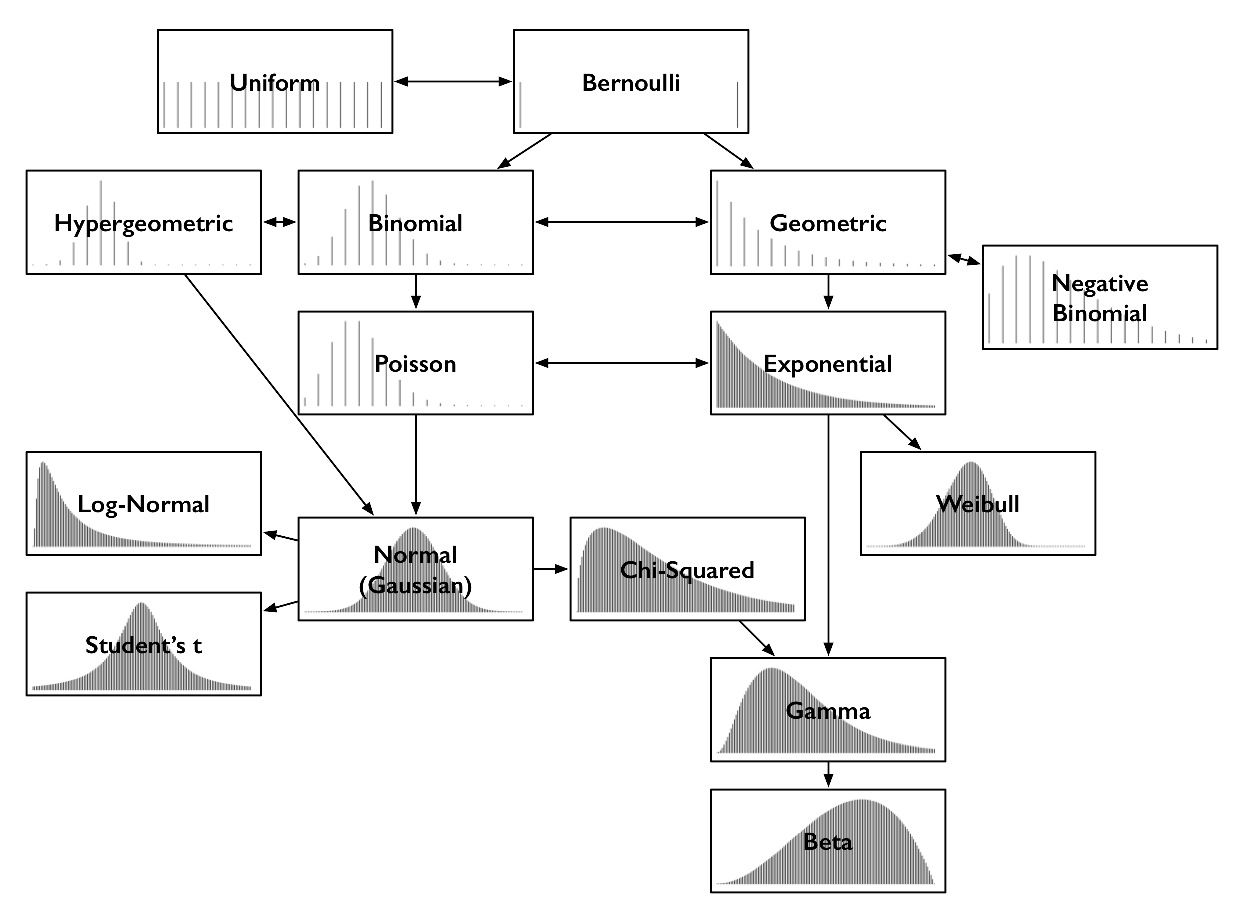
\includegraphics[height=5cm,
    angle=0]{./images/common_distributions.eps}}
\caption{Common distributions}
\label{fig:common_distributions}
\end{figure}


\subsection{Complex distribution: multimodal distributions}
\label{sec:multimodal-distributions}

You might also see complex distributions, such as two peaks that don’t disappear
with different numbers of bins, referred to as a bimodal distribution, or
multiple peaks, referred to as a multimodal distribution,
Fig.\ref{fig:multimodal_distributions}. A multimodal distribution in a sample is
usually an indication that the distribution in the population is not normal.

\begin{figure}[hbt]
  \centerline{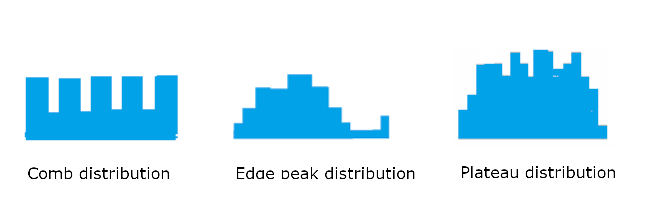
\includegraphics[height=4cm,
    angle=0]{./images/multimodal_distributions.eps}}
\caption{(A) Comb distribution, (B) Edge peak distribution (i.e. a peak at the edge), (C) Plateau distributions}
\label{fig:multimodal_distributions}
\end{figure}

\begin{itemize}
  
  \item  A multimodal distribution is a probability distribution with more than
  one peak, or “mode.” 
  
  
  \item \ldots a bimodal distribution is also multimodal, as there are $>1$ peaks.
  
  {\bf unimodal}: one peak; {\bf bimodal}: two peaks; 
  
  \item \ldots  multimodal distribution is known as a Plateau Distribution when
  there are more than a few peaks close together.
  
  \item A comb distribution is so-called because the distribution looks like a
  comb, with alternating high and low peaks.
  
  NOTE: A comb shape can be caused by rounding off. For example, if you are
  measuring water height to the nearest 10 cm and your class width for the
  histogram is 5 cm, this could cause a comb shape.
  
  \item An edge peak distribution is where there is an additional, out of place
  peak at the edge of the distribution. This usually means that you’ve plotted
  (or collected) your data incorrectly, unless you know for sure your data set
  has an expected set of outliers (i.e. a few extreme views on a survey).
  
  \item You might also see a large spike in density for a given value or small
  range of values indicating outliers, often occurring on the tail of a
  distribution far away from the rest of the density.
  
  
  \item When thinking about the cause of the multimodality, you may want to take
  a close look at your data; what may be going on is that two or more
  distributions are being mapped at the same time. This is opposed to a true
  multimodal distribution, where only one distribution is mapped.
  
\end{itemize}

\subsection{-- preprocess data}
\label{sec:pre-processing-data}

It is possible that the data does match a common probability distribution, but
requires a transformation before parametric density estimation.

For example, you may have outlier values that are far from the mean or center of
mass of the distribution. This may have the effect of giving incorrect estimates
of the distribution parameters and, in turn, causing a poor fit to the data.
These outliers should be removed prior to estimating the distribution
parameters.

Another example is the data may have a skew or be shifted left or right. In this
case, you might need to transform the data prior to estimating the parameters,
such as taking the log or square root, or more generally, using a power
transform like the Box-Cox transform.



\section{Model parameters ($\boldsymbol{\theta}$) estimation}

Suppose we have a collection of samples (i.e. data points) $X$.

The model that we use, i.e. the estimator (Sect.\ref{sec:estimator}) to capture
the properties of the data, has parameters $\boldsymbol{\theta}$.

\section{Coin flipping example}

Example: $X$ - the observatio data - is a sequence of independent coin flips,
then $\boldsymbol{\theta}$ is a single value representing the probability that a
coin comes up heads when flipped.

We want to find the most likely value for the parameters of our model.
We formulate the problem as 
\begin{equation}
\mathop{\mathrm{argmax}} P(\boldsymbol{\theta}\mid X)
\end{equation}

Using Bayes' rule, this is the same thing as
\begin{equation}
\mathop{\mathrm{argmax}} \frac{P(X \mid \boldsymbol{\theta})P(\boldsymbol{\theta})}{P(X)}.
\end{equation}

The expression $P(X)$, a parameter agnostic probability of generating the data,
 does not depend on $\boldsymbol{\theta}$ at all. So, it can be dropped without
 changing the best choice of $\boldsymbol{\theta}$.
 
In this coin-flipping example, we can also posit that we have no prior
assumption on which set of parameters are better than any others, so we may
declare that $P(\boldsymbol{\theta})$ does not depend on theta either! In other
words, the probability it comes up heads could be any value in $[0,1]$ without
any prior belief it is fair or not (often referred to as an *uninformative
prior*).
So, our best choice of $\boldsymbol{\theta}$ is the maximum likelihood estimate
for $\boldsymbol{\theta}$, or choose the value $\hat{\boldsymbol{\theta}}$ so
that once we use the model, we will maximize the likelihood/chance to get the
result same/similar to the observation $X$.

\begin{equation}
\hat{\boldsymbol{\theta}} = \mathop{\mathrm{argmax}} _ {\boldsymbol{\theta}} P(X \mid \boldsymbol{\theta}).
\end{equation}

\subsection{Define $\theta$ and estimate it}
\label{sec:maximum-likelihood}

Suppose that we have a single parameter $\theta$ representing the probability that a coin flip is heads.
Then the probability of getting a tails is $1-\theta$.


If our observed data $X$ is a sequence with $n_H$ heads and $n_T$ tails,
\begin{equation}
P(X \mid \theta) = \theta^{n_H}(1-\theta)^{n_T}.
\end{equation} 

Example: If we flip $13$ coins and get the sequence "HHHTHTTHHHHHT", which has $n_H = 9$ and $n_T = 4$
\begin{equation}
P(X \mid \theta) = \theta^9(1-\theta)^4 
\end{equation}

If we scan values of $\theta$
\begin{lstlisting}
%matplotlib inline
import d2l
from mxnet import autograd, np, npx
npx.set_np()

theta = np.arange(0, 1, 0.001)
p = theta**9 * (1 - theta)**4.

d2l.plot(theta, p, 'theta', 'likelihood')
\end{lstlisting}
, we see that the probability reach the maximum when $\hat{\theta} = 9/13$.

This example is simple as we know the closed form solution. In practice, we have
to estimate them, so having the right strategy to estimate is important, and
deep learning is a good way.


\textcolor{red}{what if we have billions of parameters and data points?}
\begin{enumerate}
  \item  too many data points?
  
  
  \item 
\end{enumerate}

\subsection{What if $\theta$ is a vector}
 
What this maximum likelihood method will give us is a way to get that number
from first principals in a way that will generalize to vastly more complex
situations.

\section{Log-likelihood: Logarithm in probability}
\label{sec:maximum-log-likelihood}

When we multiply probability of multiple data points, first notice that, if we
make the assumption that all the data points are independent (e.g. naive Bayes
classifier - Sect.\ref{sec:naive-Bayes-classifier}), we can no longer
practically consider the likelihood itself as it is a product of many
probabilities.

  Indeed, each probability is in $[0,1]$, say typically of size about $1/2$, and
  the product of $(1/2)^{1000000000}$ is far below machine precision.  We cannot
  work with that directly.
    

However, recall that the logarithm turns products to sums,
\begin{equation}
\log((1/2)^{1000000000}) = 1000000000\cdot\log(1/2) \approx -301029995.6\ldots
\end{equation}

This number fits perfectly within even a single precision $32$-bit float.  Thus, we should consider the *log-likelihood*
\begin{equation}
\log(P(X \mid \boldsymbol{\theta})).
\end{equation}

Since the function $x \mapsto \log(x)$ is increasing, maximizing the likelihood
is the same thing as maximizing the log-likelihood.

\section{Naive Bayes classifier}
\label{sec:naive-Bayes-classifier}

If we want to classify a new data point that we have never seen before we have
to make some assumptions about which data points are similar to each other.
 
The naive Bayes classifier, a popular and remarkably clear algorithm, assumes
all features are independent from each other to simplify the computation.

Example: this model to recognize characters in images, i.e. we assume each pixel
is independent from each other (Sect.\ref{sec:dataset-digits-MNIST}).


\begin{lstlisting}
%matplotlib inline
import d2l
import math
from mxnet import gluon, np, npx
npx.set_np()
d2l.use_svg_display()
\end{lstlisting}

In a classification task, we map an example into a category. 
\begin{itemize}
  \item example is an image which is represented as a single vector of $d=28*28=784$.
  
  
 $\mathbf x\in\mathbb R^d$ the features of the example (which is the transformed image with values in [0,1])
  
  \item category is a label either 0 to 9.
  
  $y\in\mathbb R$ the label. 
  
\end{itemize}

\subsection{The impossible approach}

One natural way to express the classification task is via the probabilistic
question: what is the most likely label given the features (i.e., image pixels)?
\begin{equation}
p(y  \mid  \mathbf{x}) \text{ for } y=0, \ldots,9
\end{equation}

The prediction $\hat{y}$ given by the expression:
\begin{equation}
\hat{y} = \mathrm{argmax} \> p(y  \mid  \mathbf{x}).
\end{equation}

Unfortunately, this requires that we estimate $p(y  \mid  \mathbf{x})$ for every
value of $\mathbf{x} = x_1, ..., x_d$.
If we had $30$ such binary features, that would mean that we need to be prepared
to classify any of $2^{30}$ (over 1 billion!) possible values of the input
vector $\mathbf{x}$.

\subsection{The simpler, yet also impossible approach}

We revert the problem, into a more finite output, i.e. the number of label
($d=10$), rather than using the input (d=30).


$$\hat{y} = \mathrm{argmax}_y \> p(y  \mid  \mathbf{x}) = \mathrm{argmax}_y \> \frac{p( \mathbf{x}  \mid  y) p(y)}{p(\mathbf{x})}.$$

with  $\sum_y p(y  \mid  \mathbf{x}) = 1$.

We just need to focus on  $p( \mathbf{x}  \mid  y)$. 
Using the chain rule of probability, we can express the term $p( \mathbf{x}  \mid  y)$ as

$$p(x_1  \mid y) \cdot p(x_2  \mid  x_1, y) \cdot ... \cdot p( x_d  \mid  x_1, ..., x_{d-1}, y).$$

The problem is smaller, yet  we still must estimate roughly $2^d$ parameters.

\subsection{The possible approach, yet wrong result: assumption of independence}

If we assume that {\it the features are conditionally independent of each other,
given the label}, then suddenly we are in much better shape,

\begin{equation}
\hat{y} = \mathrm{argmax}_y \> \prod_{i=1}^d p(x_i  \mid  y) p(y).
\end{equation}

We can pre-calculate (from training data): 

\begin{itemize}
  
  \item ($d\times n$ matrix):
  If we can estimate $\prod_i p(x_i=1  \mid  y)$ for every
$i$ and $y$, and save its value in $P_{xy}[i, y]$, 

here $P_{xy}$ is a $d \times n$ matrix with $n$ being the number of classes and
$y\in\{1, \ldots, n\}$.

  \item  ($n$-length vector): In addition, we estimate $p(y)$ for every $y$ and save it in $P_y[y]$, 
  
  with $P_y$ a $n$-length vector.
\end{itemize}

Then for any new example $\mathbf x$, we could compute

$$ \hat{y} = \mathrm{argmax}_y \> \prod_{i=1}^d P_{xy}[x_i, y]P_y[y],$$

for any $y$.


The assumption of conditional independence has taken the complexity of our model
from an exponential dependence on the number of features $\mathcal{O}(2^dn)$ to
a linear dependence, which is $\mathcal{O}(dn)$.

The problem now is that we do not know $P_{xy}$ and $P_y$, which are estimated given some training data first.


\subsection{-- Estimate $P_{xy}$}


Since we picked black and white images, $p(x_i  \mid  y)$ denotes the
probability that pixel $i$ is switched on for class $y$. 

Just like before we can go and count the number of times $n_{iy}$ such that an
event occurs and divide it by the total number of occurrences of $y$, i.e.,
$n_y$. 

But there is something slightly troubling: certain pixels may never be
black (e.g., for well cropped images the corner pixels might always be white).

A convenient way for statisticians to deal with this problem is to add pseudo
counts to all occurrences. Hence, rather than $n_{iy}$ we use $n_{iy}+1$ and
instead of $n_y$ we use $n_{y} + 1$.

\begin{lstlisting}
n_x = np.zeros((10, 28, 28))
for y in range(10):
    n_x[y] = np.array(X.asnumpy()[Y.asnumpy() == y].sum(axis=0))
P_xy = (n_x + 1) / (n_y + 1).reshape(10, 1, 1)

d2l.show_images(P_xy, 2, 5);
\end{lstlisting}


\subsection{-- Estimate $P_y$}

Estimating $P_y$ is not too hard. Since we are only dealing with $10$ classes,
we may count the number of occurrences $n_y$ for each of the digits and divide
it by the total amount of data $n$.

For instance, if digit 8 occurs $n_8 = 5,800$ times and we have a total of 
$n = 60,000$ images, the probability estimate is $p(y=8) = 0.0967$.


\begin{lstlisting}
X, Y = mnist_train[:]  # All training examples

n_y = np.zeros((10))
for y in range(10):
    n_y[y] = (Y == y).sum()
P_y = n_y / n_y.sum()
P_y
\end{lstlisting}

\subsection{-- Laplace smoothing}

Suppose that we did not use Laplace smoothing when estimating probabilities and
a data point arrived at testing time which contained a value never observed in
training. What would the model output?

Since we picked black and white images, $p(x_i  \mid  y)$ denotes the
probability that pixel $i$ is switched on for class $y$. Just like before we can
go and count the number of times $n_{iy}$ such that an event occurs and divide
it by the total number of occurrences of $y$, i.e., $n_y$.

There are pixels, e.g. certain pixels may never be black (e.g., for well cropped
images the corner pixels might always be white), so the probability is always
zero.

A convenient way for statisticians to deal with this problem is to add pseudo
counts to all occurrences i.e. having an additional image for that label in that
the pixel for that position is black. Hence, rather than $n_{iy}$ we use
$n_{iy}+1$ and instead of $n_y$ we use $n_{y} + 1$. This is also called *Laplace
Smoothing*. It may seem ad-hoc, however it may be well motivated from a Bayesian
point-of-view.







\subsection{-- Test the (failed) naive Bayes classifier}

Given $\mathbf x$, the following functions computes $p(\mathbf x \mid y)p(y)$ for every $y$.

\begin{lstlisting}
def bayes_pred(x):
    x = np.expand_dims(x, axis=0)  # (28, 28) -> (1, 28, 28)
    p_xy = P_xy * x + (1 - P_xy)*(1 - x)
    p_xy = p_xy.reshape(10, -1).prod(axis=1)  # p(x|y)
    return np.array(p_xy) * P_y

image, label = mnist_test[0]
bayes_pred(image)
\end{lstlisting}


\textcolor{red}{IT DOESN''T WORK}: The reason is that the probability, they are
typically numbers between $0.001$ and $1$. We are multiplying $784$ of them.
What happens is that we experience *numerical underflow*, i.e., multiplying all
the small numbers leads to something even smaller until it is rounded down to
zero.

\subsection{The possible approach, and correct result: assumption of independence}


\begin{equation}
 \hat{y} = \mathrm{argmax}_y \> \sum_{i=1}^d \log P_{xy}[x_i, y] + \log P_y[y].
\end{equation}

\begin{lstlisting}
log_P_xy = np.log(P_xy)
log_P_xy_neg = np.log(1 - P_xy)
log_P_y = np.log(P_y)

def bayes_pred_stable(x):
    x = np.expand_dims(x, axis=0)  # (28, 28) -> (1, 28, 28)
    p_xy = log_P_xy * x + log_P_xy_neg * (1 - x)
    p_xy = p_xy.reshape(10, -1).sum(axis=1)  # p(x|y)
    return p_xy + log_P_y

py = bayes_pred_stable(image)
py


# Convert label which is a scalar tensor of int32 dtype
# to a Python scalar integer for comparison
py.argmax(axis=0) == int(label)
\end{lstlisting}
 
\subsection{-- Test the naive Bayes classifier}

\begin{lstlisting}
def predict(X):
    return [bayes_pred_stable(x).argmax(axis=0).astype(np.int32) for x in X]

X, y = mnist_test[:18]
preds = predict(X)
d2l.show_images(X, 2, 9, titles=[str(d) for d in preds]);
\end{lstlisting}

The overall accuracy
\begin{lstlisting}
X, y = mnist_test[:]
preds = np.array(predict(X), dtype=np.int32)
float((preds == y).sum()) / len(y)  # Validation accuracy
\end{lstlisting}


The relatively poor performance is due to the incorrect statistical assumptions
that we made in our model: we assumed that each and every pixel are
independently generated, depending only on the label. This is clearly not how
humans write digits, and this wrong assumption led to the downfall of our overly
naive (Bayes) classifier.

REMEMBER: Modern deep networks achieve error rates of less than 0.01.



\section{Negative log-likelihood: maximum-likelihood in Deep Learning}



\subsection{negative choice: minimizing rather than mazimizing}

In Deep Learning, the last layer's output is often in the form of probability,
or likelihood.
From that, we often work with loss functions, where we wish to minimize the
loss.
We may turn maximum likelihood into the minimization of a loss by taking
$-\log(P(X \mid \boldsymbol{\theta}))$, which is the {\bf negative log-likelihood}.

Consider the coin flipping problem from before, maximizing the log-likehood is
turned into a problem of minimizing the loss function, by changing the $\theta$
parameters in steepest gradient descent.
 
$$
-\log(P(X \mid \boldsymbol{\theta})) = -\log(\theta^{n_H}(1-\theta)^{n_T}) = -(n_H\log(\theta) + n_T\log(1-\theta)).
$$

Example: here, we iterate over 10 times, but it can be more to converge
\begin{lstlisting}{lang="python"}
# Set up our data
n_H = 8675309
n_T = 25624

# Initialize our paramteres
theta = np.array(0.5)
theta.attach_grad()

# Perform gradient descent
lr = 0.00000000001
for iter in range(10):
    with autograd.record():
        loss = -(n_H * np.log(theta) + n_T * np.log(1 - theta))
    loss.backward()
    theta -= lr * theta.grad

# Check output
theta, n_H / (n_H + n_T)
\end{lstlisting}

\subsection{log- choice: simple form}

Due to independence assumptions, most probabilities we encounter in machine
learning are products of individual probabilities, which makes the use of
 log-likelihood even more important.
It turns from product calculation

$$
P(X\mid\boldsymbol{\theta}) = p(x_1\mid\boldsymbol{\theta})\cdot p(x_2\mid\boldsymbol{\theta})\cdots p(x_n\mid\boldsymbol{\theta}).
$$
which makes the calculation of derivatives too hard
$$
\begin{aligned}
\frac{\partial}{\partial \boldsymbol{\theta}} P(X\mid\boldsymbol{\theta}) & = \left(\frac{\partial}{\partial \boldsymbol{\theta}}P(x_1\mid\boldsymbol{\theta})\right)\cdot P(x_2\mid\boldsymbol{\theta})\cdots P(x_n\mid\boldsymbol{\theta}) \\
& \quad + P(x_1\mid\boldsymbol{\theta})\cdot \left(\frac{\partial}{\partial \boldsymbol{\theta}}P(x_2\mid\boldsymbol{\theta})\right)\cdots P(x_n\mid\boldsymbol{\theta}) \\
& \quad \quad \quad \quad \quad \quad \quad \quad \quad \quad \vdots \\
& \quad + P(x_1\mid\boldsymbol{\theta})\cdot P(x_2\mid\boldsymbol{\theta}) \cdots \left(\frac{\partial}{\partial \boldsymbol{\theta}}P(x_n\mid\boldsymbol{\theta})\right).
\end{aligned}
$$

to a simpler form
$$
-\log\left(P(X\mid\boldsymbol{\theta})\right) = -\log(P(x_1\mid\boldsymbol{\theta})) - \log(P(x_2\mid\boldsymbol{\theta})) \cdots - \log(P(x_n\mid\boldsymbol{\theta})),
$$
which make the calculation of derivatives easier (This requires only $n$ divides and $n-1$ sums, and thus is linear time in the inputs.)
 
$$
- \frac{\partial}{\partial \boldsymbol{\theta}} \log\left(P(X\mid\boldsymbol{\theta})\right) = \frac{1}{P(x_1\mid\boldsymbol{\theta})}\left(\frac{\partial}{\partial \boldsymbol{\theta}}P(x_1\mid\boldsymbol{\theta})\right) + \cdots + \frac{1}{P(x_n\mid\boldsymbol{\theta})}\left(\frac{\partial}{\partial \boldsymbol{\theta}}P(x_n\mid\boldsymbol{\theta})\right).
$$

\subsection{cross-entropy: has relationship to information theory}

The third and final reason to consider the negative log-likelihood is the relationship to information theory.
Information theory tells whether the model is generalized enough, i.e. whether it can encode enough information.
This is a rigorous mathematical theory which gives a way to measure the degree of information or randomness in a random variable.


The key object of study in that field is the entropy which is 

$$
H(p) = -\sum_{i} p_i \log_2(p_i),
$$

which measures the randomness of a source

If we take our negative log-likelihood and divide by the number of data points,
we get a relative of entropy known as cross-entropy.


This theoretical interpretation alone would be sufficiently compelling to
motivate reporting the average negative log-likelihood over the dataset as a way
of measuring model performance.

\chapter{Information Theory: Maths od Deep Learning}

Information comes in different format, e.g. music, written language, spoken
language, video, \ldots

Information provides a common language across disciplinary rifts: from
Shakespeare’s Sonnet to researchers’ paper on Cornell ArXiv, from Van Gogh’s
printing Starry Night to Beethoven’s music Symphony No. 5, from the first
programming language Plankalkül to the state-of-the-art machine learning
algorithms. 

\textcolor{red}{Everything must follow the rules of information theory, no matter the format.}
With information theory, we can measure and compare how much information is
present in different signals.

\section{Information: the soul}

Let’s start with the “soul” of information theory: information. Information can
be encoded in anything with a particular sequence of one or more encoding
formats.

Suppose that we task ourselves with trying to define a notion of information.
What could be are starting point?

\subsection{Example: draw a card from a deck}

Consider the following thought experiment. We have a friend with a deck of
cards. They will shuffle the deck, flip over some cards, and tell us statements
about the cards. We will try to assess the information content of each
statement.

\subsection{-- statement: I see a card}


First, they flip over a card and tell us, “I see a card.” 

Does that statement provides us any new information? 

NO: as we know for sure it is a card. 

So, the information of that statement is zero. 


\subsection{-- statement: I see a heart}

Next, they flip over a card and say, “I see a heart.” 

This provides us some information, but in reality there are only 4 different
suits that were possible, each equally likely, so we are not surprised by this
outcome. Before this statement, we can guess, with probability $1/4$, that it's a heart.

The statement brings some information, but the information is low. 

\subsection{-- statement: I see a 3 of spades}


Next, they flip over a card and say, “This is the 3 of spades.” This is more
information. Indeed there were 52 equally likely possible outcomes, and our
friend told us which one it was. Before this statement, we can guess, with
probability $1/52$, that it's a 3 of spades.

So, the statement provides a medium amount of information.

\subsection{-- statement: tell the exact order of 52 cards}


Suppose that finally they flip over every card from the deck and read off the
entire sequence of the shuffled deck. There are 52! different orders to the
deck, again all equally likely. Before this statement, the chance to tell correctly is extremely small.


So we need a lot of information to know which one it is.

\subsection{Information level = degree of surprise}

As a starting point, rather than caring about the knowledge, we may build off
the idea that information represents the degree of surprise or the abstract
possibility of the event.

For example, if we want to describe an unusual event, we need a lot information.
For a common event, we may not need much information.

\section{Information level of a single discrete event: Shannon's work (self-information)}
\label{sec:self-information}

In 1948, Claude E. Shannon published A Mathematical Theory of Communication
(Shannon.1948) establishing the theory of information. In his book, Shannon
introduced the concept of information entropy for the first time. We will begin
our journey here.

The information level is quantified in the form of {\bf number of bits required}.
Shannon introduced the terminology bit as the unit of information, which was
originally created by John Tukey. 

\textcolor{red}{What is a 'bit'?}.  Historically, an antique transmitter can
only send or receive two types of code:
0 and 1. Coincidently, binary encoding is still in common use on all modern
digital computers. Hence, a series of binary digits of length $n$ contains $n$
bits of information.

Consider a series contains $n$ bits of information: Now, suppose that for any
series of codes, each $0$ or $1$ occurs with a probability of $\frac{1}{2}$.
Hence, an event $X$ with a series of codes of length $n$, occurs with a
probability of $\frac{1}{2^n}$.

The probability $p$ (for an event to occur) is transferred to the concept of
number of bits. Shannon gave the answer by defining {\bf self-information}

$$I(X) = - \log_2 (p),$$

as the *bits* of information we have received for this event $X$.
Note that we will always use base-2 logarithms here.
So, for the sake of simplicity, the rest of this section will omit the subscript 2
in the logarithm notation, i.e., $\log(.)$ always refers to $\log_2(.)$.

\begin{lstlisting}
from mxnet import np
from mxnet.metric import NegativeLogLikelihood
from mxnet.ndarray import nansum
import random

def self_information(p):
    return -np.log2(p)

self_information(1/64)
\end{lstlisting}

\section{(Shannon) Entropy: information level in single random variable}

In 1948, Claude E. Shannon published A Mathematical Theory of Communication
(Shannon.1948) establishing the theory of information. In his book, Shannon
introduced the concept of information entropy for the first time. 
In Sect.\ref{sec:self-information}, we talked about {\bf self-information}.

As self-information only measures the information of a single discrete event, we
need a more generalized measure for any random variable of either discrete or
continuous distribution.

\subsection{Axioms of Shannon Entropy}
\label{sec:Shannon-entropy}

To be able to quantify Shannon entropy of a random variable, we rely on the
following axioms, aka {\it axioms of Shannon Entropy}.
It will turn out that the following collection of common-sense statements force
us to a unique definition of information (Csiszar.2008).

There are 3 important axioms
\begin{enumerate}
\item The information gained when observing (nearly) certain events is (nearly) zero.

\item  The information gained by observing a random variable does not depend on what
  we call the elements, or the presence of additional elements which have
  probability zero.

\item The information gained when observing two random variables is no more than
the sum of the information we gain by observing them separately. 

If they are independent, then it is exactly the sum.

\end{enumerate}

While proving this fact is beyond the scope of our text, it is important to know
that this uniquely determines the form that entropy must take. The only
ambiguity that these allow is in the choice of fundamental units, which is most
often normalized.


For any random variable $X$ that follows a probability distribution $P$ with a
probability density function (p.d.f.) or a probability mass function (p.m.f.)
$p(x)$, we measure the expected amount of information through *entropy* (or
*Shannon entropy*)

$$H(X) = - E_{x \sim P} [\log p(x)].$$

why do we use an expectation of a negative logarithm? Here are some intuitions.
\begin{enumerate}
  \item Logarithm is important as it converts multiply to sum operator.
  
  Suppose that $p(x) = f_1(x) f_2(x) \ldots, f_n(x)$, where each component
  function $f_i(x)$ is independent from each other. This means that each
  $f_i(x)$ contributes independently to the total information obtained from
  $p(x)$.
  
  We want the entropy formula to be additive over independent random variables.
  Luckily, $\log$ can naturally turn a product of probability distributions to a
  summation of the individual terms.
  
  \item Why negative Log? 
  
  Intuitively, more frequent events should contain less information than less
  common events, since we often gain more information from an unusual case than
  from an ordinary one. So, events with smaller probability should has larger
  entropy than events with larger probability.
  
  However, $\log$ is monotonically increasing with the probabilities, and indeed
  negative for all values in $[0, 1]$.
  So, we need to construct a monotonically decreasing relationship between the
  probability of events and their entropy, which will ideally be always
  positive, we add a negative sign in front of $\log$ function.
  
  \item Why Expectation function?
  
   Consider a random variable $X$. We can interpret the self-information
   ($-\log(p)$) as the amount of *surprise* we have at seeing a particular
   outcome. Indeed, as the probability approaches zero, the surprise becomes
   infinite (i.e. very very large).
   
   Similarly, we can interpret The entropy as the average amount of surprise
   from observing $X$.
   
   For example, imagine that a slot machine system emits statistical
   independently symbols ${s_1, \ldots, s_k}$ with probabilities ${p_1, \ldots,
   p_k}$ respectively. Then the entropy of this system equals to the average
   self-information from observing each output, i.e.,
   
   $$H(S) = \sum_i {p_i \cdot I(s_i)} = - \sum_i {p_i \cdot \log p_i}.$$
   
   
\end{enumerate}


\subsection{Shannon Entropy of a discrete random variable}

To be specific, if $X$ is discrete, $$H(X) = - \sum_i p_i \log p_i \text{, where } p_i = P(X_i).$$ 


Python code: MXNet library
\begin{lstlisting}
def entropy(p):
    entropy = - p * np.log2(p)
    # nansum will sum up the non-nan number
    out = nansum(entropy.as_nd_ndarray())
    return out

entropy(np.array([0.1, 0.5, 0.1, 0.3]))
\end{lstlisting}

\subsection{Shannon Entropy of a continuous random variable}

Otherwise, if $X$ is continuous, we also refer entropy as *differential entropy* 

$$H(X) = - \int_x p(x) \log p(x) \; dx.$$

We can estimate by generating many discrete values of $X$, with tiny gap between them.

\subsection{Logarithm is important to use}


For any random variable $X$ that follows a probability distribution $P$ with a
probability density function (p.d.f.) or a probability mass function (p.m.f.)
$p(x)$, we measure the expected amount of information through {\bf entropy} (or
{\bf Shannon entropy}) - Sect.\ref{sec:Shannon-entropy}.

Suppose that $p(x) = f_1(x) f_2(x) \ldots, f_n(x)$, where each component
function $f_i(x)$ is independent from each other. This means that each $f_i(x)$
contributes independently to the total information obtained from $p(x)$. As
discussed above, we want the entropy formula to be additive over independent
random variables. Luckily, $\log$ can naturally turn a product of probability
distributions to a summation of the individual terms.


\subsection{Summary of entropy}

Here, we refer to X as an event and P as the probability distribution of X.

\begin{enumerate}
  \item  * Entropy is non-negative, i.e., $H(X) \geq 0, \forall X$.

  \item * If $X \sim P$ with a p.d.f. or a p.m.f. $p(x)$, and we try to estimate
  $P$ by a new probability distribution $Q$ with a p.d.f. or a p.m.f. $q(x)$,
  then 
  
  $$H(X) = - E_{x \sim P} [\log p(x)] \leq  - E_{x \sim P} [\log q(x)], \text{ with equality if and only if } P = Q.$$  
  
  Alternatively, $H(X)$ gives a
  lower bound of the average number of bits needed to encode symbols drawn from
  $P$.
  
  \item * If $X \sim P$, then $x$ conveys the maximum amount of information if
  it spreads evenly among all possible outcomes. Specifically, if the
  probability distribution $P$ is discrete with $k$-class 
  $\{p_1, \ldots, p_k \}$, then 
  
  $$H(X) \leq \log(k), \text{ with equality if and only if } p_i =
  \frac{1}{k}, \forall x_i.$$ 
  
  If $P$ is a continuous random variable, then the
  story becomes much more complicated.  However, if we additionally impose that
  $P$ is supported on a finite interval (with all values between $0$ and $1$),
  then $P$ has the highest entropy if it is the uniform distribution on that
  interval.
  
  
\end{enumerate}


\section{(Shannon) Entropy: mutual information (between two  random variables)}

How about the entropy of a pair random variables $(X, Y)$?  We can think of
these techniques as trying to answer the following type of question, "What
information is contained in $X$ and $Y$ together compared to each separately? 
Is there redundant information, or is it all unique?"


For the following discussion, we always use $(X, Y)$ as a pair of random
variables that follows a joint probability distribution $P$ with a p.d.f. or a
p.m.f. $p_{X, Y}(x, y)$, while $X$ and $Y$ follow probability distribution
$p_X(x)$ and $p_Y(y)$, respectively.


$$H(X, Y) = -E_{(x, y) \sim P} [\log p_{X, Y}(x, y)]. $$

We can think of $H(X,Y)$ as telling us the total randomness in the pair of
random variables.  As a pair of extremes, if $X = Y$ are two identical random
variables, then the information in the pair is exactly the information in one
and we have $H(X, Y) = H(X) = H(Y)$.

On the other extreme, if $X$ and $Y$ are independent then $H(X, Y) = H(X) + H(Y)$.  

So, we have this inequality
$$
H(X), H(Y) \le H(X, Y) \le H(X) + H(Y).
$$

\subsection{pair of discrete random variables}


$$H(X, Y) = - \sum_{x} \sum_{y} p_{X, Y}(x, y) \log p_{X, Y}(x, y).$$

\subsection{pair of continuous random variables}

we define the *differential joint entropy* as 

$$H(X, Y) = - \int_{x, y} p_{X, Y}(x, y) \ \log p_{X, Y}(x, y) \;dx \;dy.$$



\begin{lstlisting}
def joint_entropy(p_xy):
    joint_ent = -p_xy * np.log2(p_xy)
    # nansum will sum up the non-nan number
    out = nansum(joint_ent.as_nd_ndarray())
    return out

joint_entropy(np.array([[0.1, 0.5], [0.1, 0.3]]))
\end{lstlisting}
This is the same *code* as before, but now we interpret it differently as working on the joint distribution of the two random variables.




\section{(Mutual) Information in Deep Learning}

Machine learning aims to extract interesting signals from data and make critical
predictions.

Information theory studies encoding, decoding, transmitting, and manipulating
information. As a result, information theory provides fundamental language for
discussing the information processing in machine learned systems.

NOTE:  many machine learning applications use the cross entropy loss.
This loss can be directly derived from information theoretic considerations.


In natural language processing, one of the most difficult problems is the
ambiguity resolution, or the issue of the meaning of a word being unclear from
context. For example, recently a headline in the news reported that “Amazon is
on fire”. You may wonder whether the company Amazon has a building on fire, or
the Amazon rain forest is on fire.

In this case, mutual information can help us resolve this ambiguity. We first
find the group of words that each has a relatively large mutual information with
the company Amazon, such as e-commerce, technology, and online. Second, we find
another group of words that each has a relatively large mutual information with
the Amazon rain forest, such as rain, forest, and tropical.


When we need to disambiguate “Amazon”, we can compare which group has more
occurrence in the context of the word Amazon. In this case the article would go
on to describe the forest, and make the context clear.






\chapter{Stats: Maths of Deep Learning}

Using a proper stastistics technique, we will know whether  when improvements
are significant, or only the result of random fluctuations in the training
process.

\begin{itemize}
  \item  The earliest reference of statistics can be traced back to an Arab scholar Al-Kindi in the $9^{\mathrm{th}}$-century
  
  He gave a detailed description of how to use statistics and frequency analysis to decipher encrypted messages
  
  \item the modern statistics arose from Germany in 1700s (after 800 years), when the researchers
  focused on the demographic and economic data collection and analysis
  
  \item Today, statistics is the science subject that concerns the collection,
  processing, analysis, interpretation and visualization of data.
\end{itemize}



\section{Descriptive vs Statistical (inference)}
\label{sec:statistical-inference}
\label{sec:descriptive-inference}

More specifically, statistics can be divided to descriptive statistics and statistical inference
\begin{enumerate}
  \item {\bf descriptive statistics}:
  summarizing and illustrating the features of a collection of observed data, which is referred to as a sample.
  
  The sample is drawn from a population, denotes the total set of similar individuals, items, or events of our experiment interests. 
  
  \item {\bf statistical inference}:
   deduces the characteristics of a population from the given samples, based on
   the assumptions that the sample distribution can replicate the population
   distribution at some degree.
   
   This often requires the choice of an estimator (Sect.\ref{sec:estimator}), and through this estimator, we conduct a {\bf hypothesis testing} (Sect.\ref{sec:hypothesis-testing})
   
\end{enumerate}

\section{Estimator}
\label{sec:estimator}

In statistics, an {\bf estimator} is {\it a function of given samples} and is
used to estimate the true parameter $\theta$. This is aka the {\bf choice of a
model} representing a truth unknown problem.

We will write $\hat{\theta}_n = \hat{f}(x_1, \ldots, x_n)$ for the estimate of
$\theta$ after observing the samples
\begin{equation}
{ x_1, x_2, \ldots, x_n }
\end{equation}.

Example:
\begin{enumerate}
  \item $\theta$ is the parameter in a Bernoulli: 
  
  If you have a number of samples from a Bernoulli random variable, then {\it the
  maximum likelihood estimate for the probability the random variable} is one can
  be obtained by {\it counting the number of ones observed and dividing by the total
  number of samples.}
  
  \item $\theta$ is the mean of a Gaussian:
  
  the maximum likelihood estimate of the mean of a Gaussian given a number of
  samples is given by the average value of all the samples.
  
  \item 
\end{enumerate}

These estimators will almost never give the true value of the parameter, but
ideally for a large number of samples the estimate will be close.
This is known as the {\bf law of large numbers}.

Example: \verb!xs! is a Gaussian random variable with mean zero and variance one.
Then we construct \verb!ys! the density 
\begin{lstlisting}{lang="python"}
import d2l
from mxnet import np, npx
import random
npx.set_np()

# Sample datapoints and create y coordinate
epsilon = 0.1
random.seed(8675309)
xs = np.random.normal(loc=0, scale=1, size=(300,))

ys = [np.sum(np.exp(-(xs[0:i] - xs[i])**2 / (2 * epsilon**2))
             / np.sqrt(2*np.pi*epsilon**2)) / len(xs) for i in range(len(xs))]

# Compute true density
xd = np.arange(np.min(xs), np.max(xs), 0.01)
yd = np.exp(-xd**2/2) / np.sqrt(2 * np.pi)

# Plot the results
d2l.plot(xd, yd, 'x', 'density')
d2l.plt.scatter(xs, ys)
d2l.plt.axvline(x=0)
d2l.plt.axvline(x=np.mean(xs), linestyle='--', color='purple')
d2l.plt.title("Sample Mean: {:.2f}".format(float(np.mean(xs))))
d2l.plt.show()
\end{lstlisting}

To see how closed the estimation of the estimator to the truth yet unknown parameter, we can use one of the 3 methods:
\begin{enumerate}
  \item  the mean squared error (L2 loss), 
  
  \item the standard deviation, and 
  
  \item statistical bias.
\end{enumerate}

\subsection{Mean squared error (L2 loss)}
\label{sec:loss-L2-loss}
\label{sec:mean-squared-error}

MSE is always non-negative.
As a measure to evaluate an estimator, the closer its value to zero, the closer
the estimator is close to the true parameter $\theta$.

\begin{equation}
\mathrm{MSE} (\hat{\theta}_n, \theta) = E[(\hat{\theta}_n - \theta)^2].
\end{equation}

NOTE: It is the most commonly used regression loss function. 

Even though MSE is a natural metric, its value can be large due to 2 sources of errors:
\begin{enumerate}
  \item The fluctuation in the estimator due to randomness in the dataset: which is explained by the 
  variance (Sect.\ref{sec:math-variance}), and
  
  The high variance usually results from a too complex model, which overfits the
  training data.
  As a result, an overfitting model is sensitive to small fluctuations in the
  data. If a model suffers from high variance, we often say it is overfitting
  and lack of flexibility
  
  \item systematic error in the estimator due to the estimation procedure: which
  is explained by the statistical bias (Sect.\ref{sec:math-statistical-bias})
  
  The bias error is commonly seen in choosing a wrong model, e.g. a simple model
  (such as a linear regression model), which cannot extract high dimensional
  relations between the features and the outputs.
  
  If a model suffers from high bias error, we often say it is underfitting or
  lack of generalization.
  
\end{enumerate}

The mean squared error can be divided into precisely two sources of error, see below: the
error from high bias and the error from high variance. 
\begin{equation}
\begin{aligned}
\mathrm{MSE} (\hat{\theta}_n, \theta) &= E[(\hat{\theta}_n - E(\hat{\theta}_n) + E(\hat{\theta}_n) - \theta)^2] \\
 &= E[(\hat{\theta}_n - E(\hat{\theta}_n))^2] + E[(E(\hat{\theta}_n) - \theta)^2] \\
 &= \mathrm{Var} (\hat{\theta}_n) + [\mathrm{bias} (\hat{\theta}_n)]^2.\\
\end{aligned}
\end{equation}

In Python
\begin{lstlisting}{lang="python"}
# Mean squared error
def mse(data, true_theta):
    return(np.mean(np.square(data - true_theta)))
\end{lstlisting}

Example: the truth $\theta$ is the mean in a normal distribution $\mathcal{N}(\theta, \sigma^2)$ 
\begin{lstlisting}
theta_true = 1
sigma = 4
\end{lstlisting}
Now, what we really have is a collection of samples
\begin{lstlisting}
sample_length = 10000
samples = np.random.normal(theta_true, sigma, sample_length)
\end{lstlisting}
Using the samples, we want to estimate the real theta by using the estimator as the mean of the samples
\begin{lstlisting}
theta_est = np.mean(samples)
theta_est
\end{lstlisting}
We ask, what is the error of this choice of the estimator?
\begin{lstlisting}{lang="python"}
mse(samples, theta_true)
\end{lstlisting}
the returned value is the same as 
\begin{lstlisting}
bias = stat_bias(theta_true, theta_est)
np.square(samples.std()) + np.square(bias)
\end{lstlisting}

\subsection{Statistical bias}
\label{sec:math-statistical-bias}
Statistical bias tells whether there is a systematic error, i.e. the estimation
procedure is accurate or not
\begin{equation}
\mathrm{bias}(\hat{\theta}_n) = E(\hat{\theta}_n - \theta) = E(\hat{\theta}_n) - \theta
\end{equation}

when $\mathrm{bias}(\hat{\theta}_n) = 0$, the expectation of the estimator
$\hat{\theta}_n$ is equal to the true value of parameter.
In this case, we say $\hat{\theta}_n$ is an unbiased estimator.  

In general, an unbiased estimator is better than a biased estimator since its
expectation is the same as the true parameter.

For example: in order to estimate the mean of a population, based on its $n$ samples, the biased estimator is 
\begin{equation}
\hat{x} = \frac{1}{n} \sum x_i
\end{equation}
, while the unbiased estimator is
\begin{equation}
\hat{x} = \frac{1}{n-1} \sum x_i
\end{equation}


\begin{mdframed}

It is worth being aware, however, that biased estimators are frequently used in
practice.  There are cases where unbiased estimators do not exist without
further assumptions, or are intractable to compute.

This may seem like a significant flaw in an estimator, however the majority of
estimators encountered in practice are at least asymptotically unbiased in the
sense that the bias tends to zero as the number of available samples tends to
infinity:
$$\lim_{n \rightarrow \infty} \mathrm{bias}(\hat{\theta}_n) = 0$$ 
\end{mdframed}

In Python
\begin{lstlisting}{lang="python"}
# Statistical bias
def stat_bias(true_theta, est_theta):
    return(np.mean(est_theta) - true_theta)
\end{lstlisting}

\subsection{Variance + Standard deviation}
\label{sec:math-variance}

*standard deviation* (or *standard error*) is defined as the squared root of the
variance. It is used to measure the randomness in the estimator. Instead of
comparing to the true population value $\theta$, we compare to the expected
sample mean $E(\hat{\theta}_n)$.
Thus we are not measuring how far the estimator tends to be from the true value,
but instead we measuring the fluctuation of the estimator itself.
 
 
We may measure the degree of fluctuation of an estimator by measuring the
standard deviation or variance of that estimator.

\begin{equation}
\sigma_{\hat{\theta}_n} = \sqrt{\mathrm{Var} (\hat{\theta}_n )} = \sqrt{E[(\hat{\theta}_n - E(\hat{\theta}_n))^2]}.
\end{equation}


\begin{itemize} 
  \item Python:  in MXNet library, we get the standard deviation  is by simply calling a.std() for a ndarray “a”, 
\end{itemize}


\section{Hypothesis testing (One-sample)}
\label{sec:hypothesis-testing}

{\bf Hypothesis testing} is the most common topics in {\bf statistical
inference} (Sect.\ref{sec:statistical-inference}), which is the field trying to
deduce the characteristics of a population from the given samples, based on
the assumptions that the sample distribution can replicate the population
distribution at some degree.
   
Via the samples, first we assume the choice of an  estimator
(Sect.\ref{sec:estimator}), and through this estimator, we conduct a {\bf
hypothesis testing}.

\begin{mdframed}
 
While hypothesis testing was popularized in the early 20th century, the first
use can be traced back to John Arbuthnot in the 1700s. John tracked 80-year
birth records in London and concluded that more men were born than women each
year.

Following that, the modern significance testing is the intelligence heritage by
Karl Pearson who invented $p$-value and Pearson’s chi-squared test
$\chi$-squared test).

William Gosset who is the father of Student’s t-distribution, and Ronald Fisher
who initialed the null hypothesis and the significance test.
\end{mdframed}

A hypothesis test is a way of  {\it evaluating some evidence (i.e. the observed
data) against the default statement about a population.} - the default statement
is called a {\bf NULL hypothesis} $H_o$ which we try to reject using the
observed data. A null hypothesis is often stated in a declarative form which
posits a relationship between variables. It should reflect the brief as explicit
as possible, and be testable by statistics theory.


The {\bf *alternative hypothesis} $H_A$ (or $H_1$) is a statement that is
contrary to the null hypothesis.

Example:
Imagine you are a chemist. After spending thousands of hours in the lab, you
develop a new medicine which can dramatically improve one's ability to
understand math. To show its magic power, you need to test it. Naturally, you
may need some volunteers to take the medicine and see whether it can help them
learn math better. How do you get started?
\begin{enumerate}
  \item  Sample selections
  
  \item 
\end{enumerate}

\section{Matplotlib package}

\begin{lstlisting}
import matplotlib.pyplot as plt
\end{lstlisting}

\section{Seaborn package (data visualization)}
\label{sec:seaborn}

Seaborn is complimentary to Matplotlib and it specifically targets statistical
data visualization. But it goes even further than that
 
``If matplotlib 'tries to make easy things easy and hard things possible',
seaborn tries to make a well-defined set of hard things easy too." 
One of these hard things or frustrations had to do with the default Matplotlib
parameters.

\begin{lstlisting}
import seaborn as sns

# Plot parameters
sns.set()
%pylab inline
pylab.rcParams['figure.figsize'] = (4, 4)
plt.rcParams['xtick.major.size'] = 0
plt.rcParams['ytick.major.size'] = 0
\end{lstlisting}
\url{https://seaborn.pydata.org/}

\url{https://elitedatascience.com/python-seaborn-tutorial}

\chapter{Regression + Classification (Machine Learning)}

\section{Choice of a model}

A model is a mathematical representation of a real world domain/problem, hoping
that the model capture the properties/behaviors of the real-world problem. 
\begin{itemize}
  \item {\bf as in linear regression}: 
  \begin{enumerate}
    \item  uni-variate, e.g. the relationship between the price of oil and the price of clothes 
  
    \item multi-variate, e.g. the relationship between the price of oil (y) and the price of clothes (x1) and the weather (x2).
  \end{enumerate}
  
  \item {\bf as in non-linear regression}
  
  \item {\bf as in classiciation} (Machine Learning: SVM, DeepLearning): y = f(x)
  
  given the input $x$, it should tell the label $y$ of that sample.
  
\end{itemize}

The choice of a model is known as an {\bf estimator} (Sect.\ref{sec:estimator}),
and thus there are errors that come with such choice
(Sect.\ref{sec:loss-L2-loss}). The quality of a model 
\begin{enumerate}
  \item high {\bf bias} error: it means the choice of model is too simple, and thus cannot capture the more-complicated relationship 
  
  \item high {\bf variance} error: it means the learned model is overfitting the samples data, and thus is sensitive to small fluctuation in the samples
  
\end{enumerate}

\chapter{Distribution: Maths of Deep Learning}

\begin{enumerate}
  \item  Bernoulli random variables can be used to model events with a yes/no outcome.
  \item  Discrete uniform distributions model selects from a finite set of possibilities.
  \item  Continuous uniform distributions select from an interval.
  \item  Binomial distributions model a series of Bernoulli random variables, and count the number of successes.
  \item  Poisson random variables model the arrival of rare events.
  \item  Gaussian random variables model the result of adding a large number of independent random variables together.
\end{enumerate}


\section{Bayesian: importance sampling with SIR algorithm (1987, 1988)}

Suppose you have some knowledge (i.e. assumption) about distribution of
parameters/inputs, i.e. pre-model distribution.
Of course, you can draw samples from this pre-model distribution. 

Consider reading Sect.\ref{sec:probability-density-estimation}.

You know run these samples to the (deterministic/mechanistic) model, you get the quality of the output. So, the quality of the output gives you
the information about the validity of the input, i..e. the imporantce.

To get the right distribution of the input, once we incorporate the knowledge from the model, we can apply 
{\bf sampling-importance-resampling} algorithm (Rubin 1987, 1988).

\begin{itemize}
  \item  draw large samples of size $k$ of inputs $\theta$ from $p^{[\theta]}(\theta)$
  
  \item  test the importance of the sample: so that we can assign a (importance
  sampling) weight $w_i$ to each input sample $\theta_i$
  
  \item {\bf resampling}: draw a second sample of size $l$ from discrete distribution with value $\theta_i$ and associated probabilities $w_i$.
\end{itemize}

The second sample is approximately a sample from the postmodel distribution and it is the
basis for inference about inputs outputs and quantities of interest in the Bayesian synthesis method


\chapter{Linear NN: }

Before we get into the details of deep neural networks, we need to cover the basics of neural network training.
The entire training process
\begin{enumerate}
  \item collect samples correctly
  
  This includes preprocessing data
  
  \item defining simple neural network architectures
  
  \item specifying a loss function,
  
  \item initialize the weights
  
  \item train the models, i.e. learning the weights
\end{enumerate}

Classic statistical learning techniques such as linear and logistic regression
can be cast as shallow neural networks, which focus on finding the relationship
between input and output.

Machine learning, on the other hand, is most often concerned with prediction.
Not every prediction problem is a classic regression problem. 

In classification problems, the goal is to predict membership among a set
of categories.

\section{Linear regression}


In the natural sciences and social sciences, the purpose of regression is most
often to characterize the relationship between the inputs and outputs.
\begin{itemize}
  \item  data points $\mathbf{x}$ and corresponding real-valued targets $y$.
\end{itemize}

Regression problems pop up whenever we want to predict a numerical value, e.g.
predicting prices (of homes, stocks, etc.), predicting length of stay (for
patients in the hospital), demand forecasting (for retail sales), among
countless others.

\begin{mdframed}

First, we assume that the relationship between the features $\mathbf{x}$ and targets
$y$ is linear, i.e., that $y$ can be expressed as a weighted sum of the inputs
$\textbf{x}$, give or take some noise on the observations. 


Second, we assume that any noise is well-behaved (following a Gaussian
distribution).

\end{mdframed}
 
\subsection{weights and bias}

Example: The target (price) can be expressed as a weighted sum of the features
(area and age):

$$\mathrm{price} = w_{\mathrm{area}} \cdot \mathrm{area} + w_{\mathrm{age}} \cdot \mathrm{age} + b.$$

Here, $w_{\mathrm{area}}$ and $w_{\mathrm{age}}$ are called weights, and $b$ is
called a bias (also called an offset or intercept).

The weights determine the influence of each feature on our prediction and the
bias just says what value the predicted price should take when all of the
features take value $0$.

Even if we will never see any homes with zero area, or that are precisely zero
years old, we still need the intercept or else we will limit the expressivity of
our linear model.

\subsection{\ldots matrix-vector form}

In ML, we usually work with high-dimensional datasets, so it is more convenient
to employ linear algebra notation. When our inputs consist of $d$ features, we
express our prediction $\hat{y}$ as

$$\hat{y} = w_1 \cdot x_1 + ... + w_d \cdot x_d + b.$$

One data point: Collecting all features into a vector $\mathbf{x}$ and all weights into a vector
$\mathbf{w}$, we can express our model compactly using a dot product:

$$\hat{y} = \mathbf{w}^T \mathbf{x} + b.$$ 

For a collection of data points $\mathbf{X}$, the predictions $\hat{\mathbf{y}}$
can be expressed via the matrix-vector product (Sect.\ref{sec:math-matrix}):

$${\hat{\mathbf{y}}} = \mathbf X \mathbf{w} + b.$$

\subsection{\ldots finding the parameters: loss function and update rule}

We will need two more things: (i) a quality measure for some given model (i.e. the loss function $L$); and
(ii) a procedure for updating the model to improve its quality.

$$\mathbf{w}^, b^ = \operatorname*{argmin}_{\mathbf{w}, b}\ L(\mathbf{w}, b).$$

\textcolor{red}{Loss function as squared error}: the squared error for a given data point is given by:

$$l^{(i)}(\mathbf{w}, b) = \frac{1}{2} \left(\hat{y}^{(i)} - y^{(i)}\right)^2.$$

The constant $1/2$ makes no real difference but will prove notationally convenient, cancelling out when we take the derivative of the loss. 

To measure the quality of a model on the entire dataset, we simply average (or equivalently, sum) the losses on the training set.

$$L(\mathbf{w}, b) =\frac{1}{n}\sum_{i=1}^n l^{(i)}(\mathbf{w}, b) =\frac{1}{n} \sum_{i=1}^n \frac{1}{2}\left(\mathbf{w}^\top \mathbf{x}^{(i)} + b - y^{(i)}\right)^2.$$

\textcolor{red}{Update rule by taking the derivative of the loss}:
When training the model, we want to find parameters ($\mathbf{w}^i, b^i$) that minimize the total loss across all training samples:



\section{Linear regression using libraries}


\subsection{Gluon}

\section{Softmax regression}




\chapter{Simulation (mechanistic) models}

Simulation models are widely used in applied scientic disciplines.
Given a set of inputs(i.e. parameters) a simulation model produces a set of
outputs.

However, in any specific application the values of necessary parameters may be
unknown. In this case, physical observations of the system in the specific
context are used to learn about the unknown parameters. The process of fitting
the model to the observed data by adjusting the parameters is known as
calibration (Sect.\ref{sec:calibration-model-parameters}).


Example:
\begin{itemize}
  \item  Inputs to biological population dynamics model may include mortality and reproduction rates for various
age groupshabitat parametersand harvest information

Outputs, at a given time point, would then typically include current population abundance and age structure

  \item In a model of soil pollutiontypical inputs include
soil density deposition velocity and air pollutant concentration

The output would be a measure of pollutant concentration in the soil.

\end{itemize}

Simulation models $M$ are usually designed to capture some underlying mechanism or
natural process and they are often deterministic (other notation: RGZ(1995) used $\Phi$).

\begin{equation}
M: \theta \rightarrow \phi
\end{equation}
with $\theta$ (parameter sets $\in \mathcal{R}^n$), $\phi$ (output - $\in \mathcal{R}^p$). 
We can write: $\phi = M(\theta)$.
If $ p < n$, the model is non-invertible. In these cases, a single value of the output vector may result from many different values of the input vector.


\begin{mdframed}

For many scientistsa mechanism is most naturally modeled using a deterministic
approach The deterministic simulation model is viewed as a useful approximation
of reality that is easier to build and interpret than a stochastic model.

On one handdeterminism permits ease of model construction and understanding 
on the otherignoring stochastic variation can result in a loss of modelling
realism In some casesthe positive aspects of the former are considered to
outweigh the disadvantages of the latter In other situationsthe random
variation is thought to account for little of the overall uncertaintyin which
case a deterministic model closely approxi mates a stochastic counterpart
Ignoring random variation can then be thought of as a modelling assumption.

\end{mdframed}

\section{Complexity of a deterministic model}

A deterministic simulation model is not necessarily a simple model Some
simulation models are extremely complicated with large numbers of inputs and
outputs.
The relationships between variables can be highly complex and the models are
often noninvertible a xed single set of outputs can be generated by multiple
sets of inputs.

Thus, taking reliable account of parameter and model uncertainty is crucialperhaps
even more so than in standard statistical modelsyet this is an area that has
received little attention from statistician

\subsection{-- example: population dynamics models PDMs)}

A population dynamics model relates the population at time $(t+1)$ to the
population at time $t$. Age-structured population dynamics models relate the
population aged a at time $(t+1)$ to the population at each age at time $t$.
 

 

\subsection{calibration (tuning parameters): simulation model validation}
\label{sec:calibration-model-parameters}

Calibration is typically effected by ad hoc fitting, and after calibration the
model is used, with the fitted input values, to predict the future behaviour of
the system.

The most common way of specifying the inputs to such a model is a kind of ad
hoc trialand error or tuning approach.

Inputs can include parameters that quantify aspects of the underlying
mechanisminitial conditionsand control parameters that specify how the simulation is to be
run.

\subsection{-- ad-hoc approach}

\begin{mdframed}
The tuning approach starts with an initial guess at appropriate values of the inputsbased
on professional knowledge and expertiseinformation in the relevant scientic literatureand so
on.

If the outputs seem plausiblethe initial guess is used  otherwise the guess is
modied.

The process iterates until a satisfactory set of inputs is foundie one that
seems reasonable in itself and also produces plausible outputs.

\end{mdframed}

\subsection{-- Bayesian approach: from pre-model distribution to post-model distribution}

However, the information about plausibility of input and output values is
encoded explicitly using a probability distribution called the {\bf pre=-model
distribution}.


Wolpert (1995) showed that Bayesian synthesis was subject to the Borel paradox
so that in principle the results could depend on the models parameterization.
In their response to Wolpert, Raftery et al. (1995b)argued that the effect
of the Borel paradox on the results was likely to be small in practice.
Neverthelessany method that is subject to the Borel paradox is unsatisfactor

 
We let $\psi$ denote the set of quantities of interest, which may be model
inputs, model outputs, or functions of both and typically will be functions of
$\phi$, and/or $\theta$. Then $p(\theta, \phi)$ represents the {\bf joint premodel distribution} - which
summarizes all available information about $\theta$ and $\phi$, except that embodied in the model itself. 

RGZ(1995) defined that the joint distribution $\pi(.)$ of ($\theta, \phi$) given
the model is simply the {\bf restriction of the premodel distribution to the
sub-manifold defined by the model } ${(\theta, \phi): \phi=M(\theta)}$, and is
called {\bf post-model distribution}.

\begin{equation}
\pi(\theta, \phi) = \left\{ 
\begin{array}{l}
p(\theta, M(\theta)) ; \text{ if} \phi = M(\theta) \\
0 ; \text{ otherwise} 
\end{array}
\right.
\end{equation}

{\bf The marginal post-model distribution} of $\theta$, i.e. the distribution
$\pi$ without any reference to $\phi$, is
\begin{equation} 
\pi^{[theta]}(\theta) \propto p(\theta, M(\theta))
\end{equation}
or equivalently
\begin{equation}
\pi^{[theta]}(\theta) = p^{[\phi|\theta]}(\theta| \phi = M(\theta))
\end{equation}
For marginal and conditional distributions RGZ used superscripts in square brackets to show to
what the distribution applies.

\subsection{---- Borel paradox}
\label{sec:Borel-paradox}

\begin{equation}
\pi^{[theta]}(\theta) = p^{[\phi|\theta]}(\theta| \phi = M(\theta))
\end{equation}

Wolpert (1999, in a discussion of RGZ, pointed out that a conditional
distribution of the form in the above equation is ill-defined, leading to the
so-called {\bf Borel paradox}.
One consequence of the Borel paradox is that the postmodel distribution depends
on how the simulation model $M$ is parameterized. Possibility, using the
arbitrrily extreme values of parameters, one can in principle obtain any density
as the post-model distribution.

\begin{mdframed}

In probability theory, the Borel–Kolmogorov paradox (sometimes known as Borel's
paradox) is a paradox relating to conditional probability with respect to an
event of probability zero (also known as a null set).
Such conditioning is indeterminate, and the resulting conditional density
depends on how the space is parameterized, and thus can affect the outcome of
the probability.

\end{mdframed}


However, if it could be reformulated as a standard Bayesian procedure, then the
Borel paradox would vanish. This is the motivation behind Bayesian melding.

\subsection{--- Bayesian meldding}

In a Bayesian context it is useful to decompose the premodel distribution into prior and likeli
hood components

Under the assumption that premodel information about inputs is independent
of that about outputs


\subsection{quantifying parameter uncertainty}

While little attention tends to be paid to uncertainty about the inputsa
sensitivity analysis is often run to see if the final conclusions are sensitive
to the precise values of the inputs used.

If the conclusions turn out to be insensitive to the inputsall is well
Howeverif there is some sensitivityit is not clear what should be done
except to note it in the report. This seems somewhat unsatisfactoryas there
will often be a degree of sensitivity to the inputs of a complex model.

Sensitivity is a form of uncertaintyand that it should be taken into
account explicitly when drawing conclusions.




\chapter{Deep Learning}
\label{chap:deep-learning}


Machine learning and its sub-topic, deep learning, are gaining momentum because
machine learning allows computers to find hidden insights without being
explicitly programmed where to look.

Deep learning has showed successes in machine vision, speech recognition and
natural language processing show the technology is ripe for adoption by enterprise.

Deep learning refers to neural networks (Sect.\ref{sec:neural-network}) with
multiple hidden layers that can learn increasingly abstract representations of
the input data. Deep learning is a type of machine learning.

Machine Learning algorithms like GLM (Sect.\ref{sec:GLM}), Naive Bayes
(Sect.\ref{sec:Naive-Bayes}), Random Forest (Sect.\ref{sec:Random-Forest}),
Gradient Boosting (Sect.\ref{sec:Gradient-Boosting}), Neural Networks or others
to analyze historical data to find insights.
This step includes tasks like collection, preparation or transformation of data. 

Here, we discuss different frameworks to help creating 
any neural-network architecture
\begin{enumerate}
  \item  any standard NN architecture, either deep feed-forward, CNN or RNN
    
  \item  
\end{enumerate}


Neural networks operate by interspersing layers of linear transformations with
non-linear operations (Sect.\ref{sec:activation-function-nonlinearity}).


\section{Activation function}
\label{sec:activation-function-nonlinearity}	

Recall what you have learnt from affine transformation
(Sect.\ref{sec:affine-transformation}), and its special case {\bf linear
transformation} (Sect.\ref{sec:linear-transformation}).

We can have some form of non-linear transformation using bias vector. But a true
non-linear transformation requires using an activation function.

The idea is that instead of treating the result of the affine transformation as
the output of the node, we add an additional step, i.e. running the linear
combination through a nonlinear activation function and treating that as the
unit output, Fig.\ref{fig:node_neuralnet}.


\begin{figure}[hbt]
  \centerline{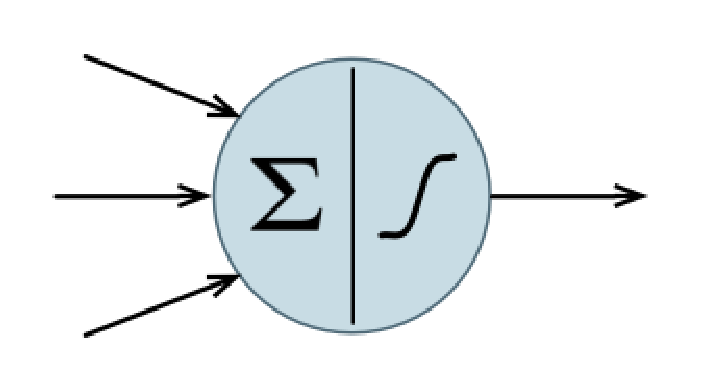
\includegraphics[height=4cm,
    angle=0]{./images/node_neuralnet.eps}}
\caption{A typical unit/node in the neural net which does weighted sum of inputs
(i.e. linear transformation) and then applied the result to a non-linear
activation function}
\label{fig:node_neuralnet}
\end{figure}


There are a whole bunch of different options available for which activation
function you use (Sect.\ref{sec:activation-function-nonlinearity}).



\begin{figure}[hbt]
  \centerline{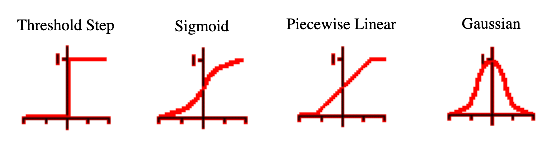
\includegraphics[height=3cm,
    angle=0]{./images/activation_functions.eps}}
\caption{Activation functions}
\label{fig:activation_functions}
\end{figure}


It used to be that you just used a sigmoid function by default, but nowadays
people use different activation functions for different purposes.
\begin{enumerate}
  \item {\bf sigmoid function}: {\bf tanh function} and {\bf logistic function}
  
  
  It models the frequency of action potentials, or firing, of biological
  neurons, i.e. it starts with small values, but can jump to a much higher value
  once it surpass a given threshold. The output is boud within a range.
  
  The first is a hyperbolic tangent that ranges from -1 to 1
 \begin{equation}
 y(u_i) = \tanh(u_i) = \frac{1}{1 + e ^{-u_i}}
 \end{equation}
 
  the other is the logistic function, which is similar in shape with tanh
  function but ranges from 0 to 1.

  \item {\bf ReLU function}
  
  The rectifier linear unit (ReLU) is more frequently used as one of the
  possible ways to overcome the numerical problems related to the sigmoids.
  
  
  \item {\bf  rectifier and softplus functions}
  
  \item {\bf radial basis functions} (more specialized activation function)
\end{enumerate}

\section{Multilayer perceptron ($\ge 1$ hidden layer)}

A multilayer perceptron (MLP) is a class of feedforward artificial neural
network (ANN).  An MLP consists of at least three layers of nodes: an input
layer, a hidden layer and an output layer.

Multilayer perceptrons are sometimes colloquially referred to as "vanilla" 
neural networks, especially when they have a single hidden layer.

Except for the input nodes, each node is a neuron that uses a nonlinear
activation function. MLP utilizes a supervised learning technique called
backpropagation for training.

\begin{figure}[hbt]
  \centerline{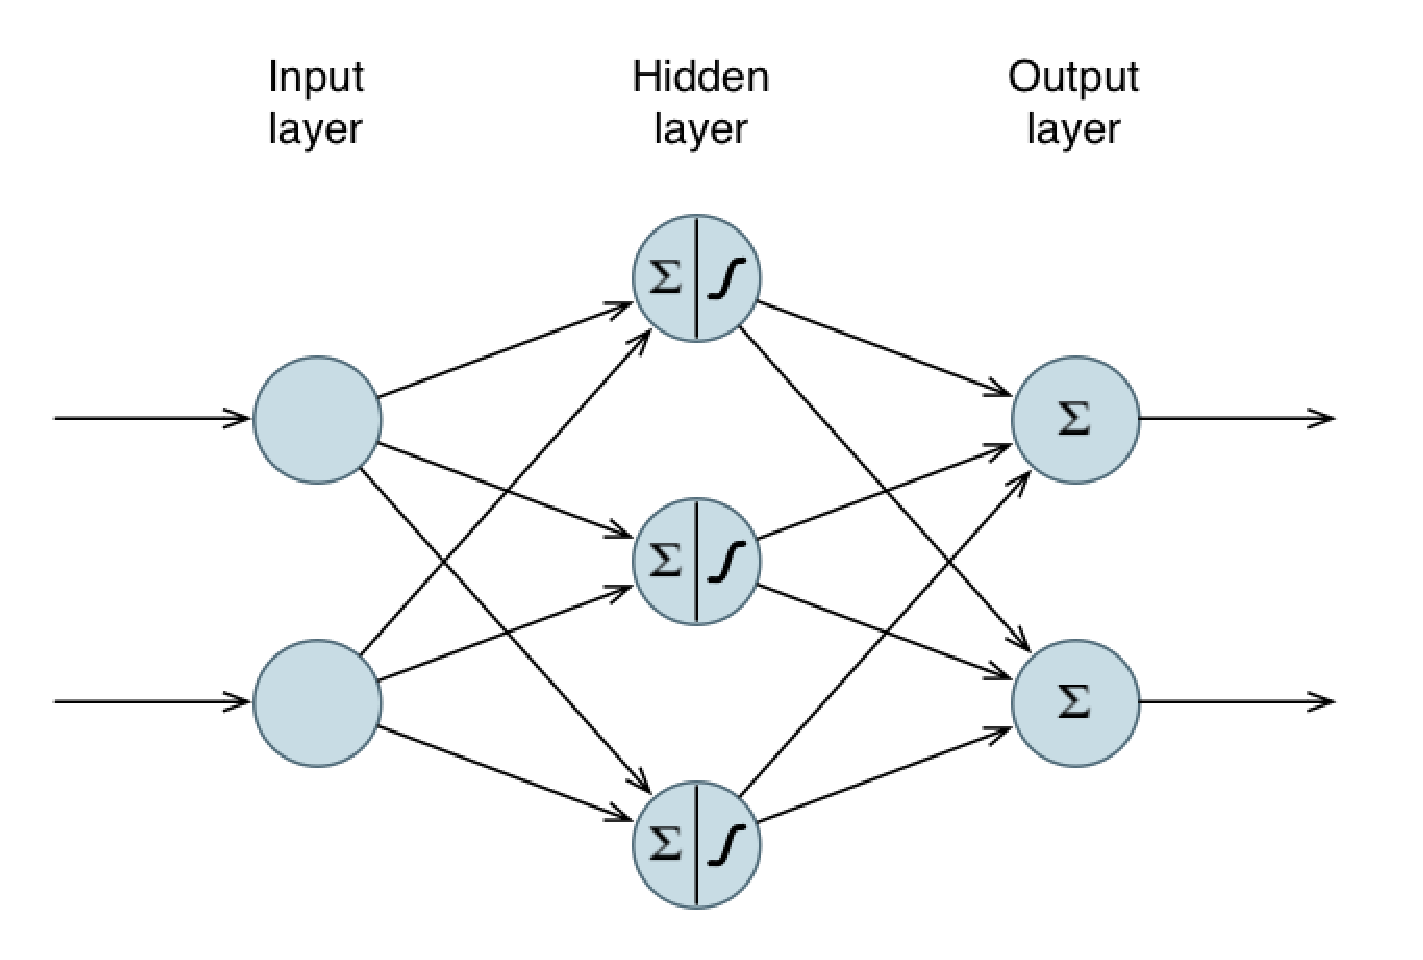
\includegraphics[height=6cm,
    angle=0]{./images/perceptron_neuralnet.eps}}
\caption{A feed-forward neural net, in that the bias is suppressed}
\label{fig:perceptron_neuralnet}
\end{figure}

\subsection{McCulloch-Pitts neuron (1943)}

 Warren McCulloch and Walter Pitts  in their 1943 paper, "A Logical Calculus of
 Ideas Immanent in Nervous Activity," contended that neurons with a binary
 threshold activation function were analogous to first order logic sentences.
 \begin{equation}
y = \phi \left( \sum_{i=1}^n w_i x_i \right)
 \end{equation}
\textcolor{red}{IMPORTANT}:  It only allowed for binary inputs and outputs, it
only used the threshold step activation function and it did not incorporate
weighting the different inputs.

\begin{mdframed}

Because of that, it has some serious limitation. In particular, there is no
threshold we can find to solve neither the “exclusive or” function (XOR), nor
the “exclusive nor” function (XNOR).

\end{mdframed}

 The McCulloch-Pitts neuron worked by inputting either a 1 or 0 for each of the
 inputs, where 1 represented true and 0 false.
 
 Thus, in order to represent the “and” function, we set the threshold at 2.0 and
 come up with the following truth table:
 \begin{verbatim}
 x1   x0     y
 0    0      0
 1    0      0
 0    1      0
 1    1      1
 \end{verbatim}

This follows also for the “or” function, if we switch the threshold value to 1.  
 \begin{verbatim}
 x1   x0     y
 0    0      0
 1    0      1
 0    1      1
 1    1      1
 \end{verbatim}

This type of artificial neuron could also be used to solve the “not” function,
which would have only one input, as well as, the NOR and NAND functions.


\subsection{Rosenblatt neuron (1950+): McCulloch-Pitts neuron + Hebbs knowledge}

In his book in 1949, The Organization of Behavior, he proposed what has come to
be known as Hebb’s rule.  He states, “When an axon of cell A is near enough to
excite a cell B and repeatedly or persistently takes part in firing it, some
growth process or metabolic change takes place in one or both cells such that
A’s efficiency, as one of the cells firing B, is increased.”
 
Hebb was proposing not only that, when two neurons fire together the connection
between the neurons is strengthened, but also that this activity is one of the
fundamental operations necessary for learning and memory.

Frank Rosenblatt, using the McCulloch-Pitts neuron and the findings of Hebb,
went on to develop the first perceptron, in that the weight between two
connected neurons can be modified. Thus, an input of 1 may be given more or less
weight, relative to the total threshold sum.

Example: A perceptron has a total of five inputs a1 through a5 with each having
a weight of w1 through w5.

The activation function used by McCulloch and Pitts was the threshold step
function.  However, other functions that can be used are the Sigmoid, Piecewise
Linear and Gaussian activation functions (Sect.\ref{sec:activation-function-nonlinearity}).


\subsection{-- Perceptron neural network as a hardware unit}

A single MLP neuron is a simple linear classifier, but complex non-linear
classifiers can be built by combining these neurons into a network.

Started in 1950s, {\bf perceptron} is a simple algorithm intended to perform
binary classification; i.e. it predicts whether input belongs to a certain
category of interest or not.
Frank Rosenblatt, godfather of the perceptron, popularized it as a device rather
than an algorithm. Rosenblatt, a psychologist who studied and later lectured at
Cornell University, received funding from the U.S. Office of Naval Research to
build a machine that could learn. His machine, the Mark I perceptron, looked
like this. 


Rosenblatt built a single-layer perceptron. It was, therefore, a shallow neural
network, which prevented his perceptron from performing non-linear
classification, such as the XOR function (an XOR operator trigger when input
exhibits either one trait or another, but not both; it stands for “exclusive
OR”), as Minsky and Papert showed in their book.

The initial hype about its performance led to a rebuttal by Minsky and Papert,
and wider spread backlash that cast a pall on neural network research for
decades.

A perceptron is a linear classifier; that is, it is an algorithm that classifies
input by separating two categories with a straight line
\begin{equation}
y = \phi \left( \sum_{i=1}^n w_i x_i + \mathbf{b} \right) = \phi\left( \mathbf{w}^T \mathbf{x} + \mathbf{b} \right)
\end{equation}
$\phi$ is the non-linear activation function.

A neural net winter that wholly thawed only with Geoff Hinton’s research in the
2000s, the results of which have since swept the machine-learning community.



\section{Radial basis network}
\label{sec:radial-basis-network}

Proposed by Broomhead and Lowe (1988) while working for  Royal Signals and Radar
Establishment, UK.

Each RBFN neuron stores a “prototype” vector which capture the 'distance' to the
input vector. Given a new input, each neuron computes the Euclidean distance
between the input and its prototype; and outputs a value between 0 and 1 which
is a measure of similarity - the output of the RBF activation function.

, and the importance of that ``prototype" is reflected via the
weight, when combining all the prototype from all hidden neurons, into making
the prediction of output label


 The shape of the RBF neuron’s response is typically a bell curve,
i.e. Gaussian function. The neuron’s response value is also called its
“activation” value.

The score is computed by taking a weighted sum of the activation values from
every RBF neuron. By weighted sum we mean that an output node associates a
weight value with each of the RBF neurons (that it receives the connection), and
multiplies the neuron’s activation by this weight before adding it to the total
response.  Every output node has its own set of weights. {\it The output node
will typically give a positive weight to the RBF neurons that belong to its
category, and a negative weight to the others.}

Roughly speaking, if the input more closely resembles the class A prototypes
than the class B prototypes, it is classified as class A.

Radial basis function (RBF) networks typically have three layers: an input
layer, a hidden layer with a non-linear RBF activation function and a linear
output layer.
\begin{itemize}
  \item input vector ($n$ units): $\mathcal{R}^n$
  
  In the basic form all inputs are connected to each hidden neuron.

  \item hidden layer: $N$ hidden neurons (known as RBF neurons)
  
  Each RBF neuron behaves like a Gaussian function, with the center represents
  the {\bf prototype} it represents. A Gaussian function has the form
  \begin{equation}
  f(x) = \frac{1}{\sigma \sqrt{2\pi}} e^{-\frac{(x-\mu)^2}{2\sigma^2}}
  \end{equation}
  
  For the activation function, $\phi$, we aren’t directly interested in the
  value of the standard deviation, $\sigma$, so we make a couple simplifying
  modifications 
  \begin{itemize}
    \item remove the coefficient: this term normally controls the height of the Gaussian

  Here, without the scaling coefficient, the function produces output in the range 0 to 1.
      
   In fact, the height is also controled with the weights applied by the output
   nodes.
   During training, the output nodes will learn the correct coefficient or
   “weight” to apply to the neuron’s response.
     
    \item replace the inner coefficient  $\frac{1}{2 * \sigma^2)}$, with a
    single parameter ‘beta’.
    
    This beta coefficient controls the width of the bell curve.
  \end{itemize}
  
  and turning that into a RBF activation function as
  \begin{equation}
  \phi(x) = e^{-\beta || x - \mu||^2}
  \end{equation}
  
  The double bar notation in the activation equation indicates that we are
  taking the Euclidean distance between x and mu, and squaring the result.
 
\begin{mdframed}

Each RBF neuron will produce its largest response when the input is equal to the prototype vector
As we move out from the prototype vector, the response falls off exponentially.

In an all-to-all connection, every RBF neuron in the network will have some
influence over the classification decision.
The exponential fall off of the activation function, however, means that the
neurons whose prototypes are far from the input vector will actually contribute
very little to the result.

\end{mdframed} 
  
  \item output: a scalar value $\mathcal{R}$
  
  
  \item the activation function for a given hidden unit $i$-th depends on the
  relative distance of that unit t with the center hidden unit
  
  The center vectors $c_i$ of the RBF functions in the hidden layer are chosen.
  This step is unsupervised, and can be performed in several ways; centers can
  be randomly sampled from some set of examples, or they can be determined using
  k-means clustering.
  
  
\end{itemize}


The training process for an RBFN consists of selecting three sets of parameters:
the prototypes (mu) and beta coefficient for each of the RBF neurons, and the
matrix of output weights between the RBF neurons and the output nodes.

\textcolor{red}{The norm is typically taken to be the Euclidean distance (although the
Mahalanobis distance appears to perform better in general)}


APPLICATION:  function approximation, time series prediction, classification, and system control. 

\url{https://mccormickml.com/2013/08/15/radial-basis-function-network-rbfn-tutorial/}

\subsection{how many RBF neurons, i.e. number of prototypes?}

An RBFN can define any arbitrarily complex decision boundary. In other words,
you can always improve its accuracy by using more RBF neurons.
Remember that each RBF neuron encodes one prototype. So the number of prototypes
equatls to the number of hidden RBF neurons.

What it really comes down to is a question of efficiency–more RBF neurons means
more compute time, so it’s ideal if we can achieve good accuracy using as few
RBF neurons as possible.


One of the approaches for making an intelligent selection of prototypes is to
perform k-Means clustering on each category samples from your training set and
to use the cluster centers as the prototypes.

How many clusters to pick per class has to be determined “heuristically”. Higher
values of k mean more prototypes, which enables a more complex decision boundary
but also means more computations to evaluate the network.

Example: I ran k-means clustering with a k of 10 twice, once for the first
class, and again for the second class, giving me a total of 20 clusters.


\subsection{ select $\beta$ (beta)}


If you use k-means clustering to select your prototypes, then one simple method
for specifying the beta coefficients is to set sigma equal to the average
distance between all points in the cluster and the cluster center.
\begin{equation}
\sigma = \frac{1}{m} \sum_{i=1}^m ||x_i - \mu||
\end{equation}
$\mu$ is the cluster centroid, m is the number of training samples belonging to this cluster

$\beta = \frac{1}{2 \sigma^2}$

\subsection{ learn output weights}


The final set of parameters to train are the output weights. These can be
trained using gradient descent (also known as least mean squares).

First, for every data point in your training set, compute the activation values
of the RBF neurons. These activation values become the training inputs to
gradient descent.

\subsection{Disadvantage of RBF network?}


The size of the RBFs network were always trained by k-means.


When your input is an image of size 128x128x3=50,000 inputs.

\url{https://www.cc.gatech.edu/~isbell/tutorials/rbf-intro.pdf}


\section{Convolutional Neural Network}
\label{sec:convolutional-neural-network}


In a nutshell, Convolutional Neural Networks (CNN's) are multi-layer neural
networks (sometimes up to 17 or more layers) that assume the input data to be
images. 

\url{http://cs231n.github.io/convolutional-networks/}


Consider you have an input, which can be 2D image or 3D images. 
\begin{verbatim}

INPUT [32x32x3] will hold the raw pixel values of the image, 
      in this case an image of width 32, height 32, 
      and with three color channels R,G,B.


\end{verbatim}

This input is
passed into the first layer, each node in the layer {\bf see} portion of the image, e.g.
\begin{itemize}
  \item one node handle 1 pixel
  
  \item one node handle 3x3 pixels 
  
  \item one node handle 5x5 pixels
\end{itemize}
Each one corresponds to a covolution operator.

\begin{verbatim}
CONV layer will compute the output of neurons that are connected to 
     local regions in the input, 
     each computing a dot product between their weights and a small region 
     they are connected to in the input volume. 
     
     This may result in volume such as [32x32x12] 
     if we decided to use 12 filters.

\end{verbatim}

NOTE: After one CONV, we can apply
\begin{verbatim}
RELU layer will apply an elementwise activation function, 
      such as the max(0,x) thresholding at zero. 
      This leaves the size of the volume unchanged ([32x32x12]).

POOL layer will perform a downsampling operation along 
     the spatial dimensions (width, height), 
     resulting in volume such as [16x16x12].

\end{verbatim}

Note that some layers contain parameters (bias, weights) and/or hyperparameters
(stride, zero padding, number of filters, etc.) and other don’t.
\begin{itemize}
  
  \item those with parameters: CONV/FC layers perform transformations that are a
  function of not only the activations in the input volume, but also of the
  parameters (the weights and biases of the neurons). The RELU/POOL layers will
  implement a fixed function.
  
 
  \item those with hyperparameters: Each Layer may or may not have additional
  hyperparameters (e.g. CONV/FC/POOL do, RELU doesn’t)
  
\end{itemize}

NOTE:
\begin{itemize}
  
  \item  There are a few distinct types of Layers (e.g. CONV/FC/RELU/POOL are by far the most popular)

  \item Each Layer accepts an input 3D volume and transforms it to an output 3D
  volume through a differentiable function.
  
\end{itemize}

\subsection{logits, i.e. the softmax argument}
\label{sec:logits}


After multiple layers, each apply one {\bf convolution filter} on one or many
elements in the incoming-input, we can convert them into a N-dimensional vector
of real-values. 
\begin{verbatim}

FC (i.e. fully-connected) layer will compute the class scores, 
        resulting in volume of size [1x1x10] 
        in the case of MNIST-image, 
        
        where each of the 10 numbers correspond to a class score, 
        such as among the 10 categories of CIFAR-10. 
        
        As with ordinary Neural Networks and as the name implies, 
        each neuron in this layer will be connected to 
        all the numbers in the previous volume.

\end{verbatim}

Typically, this is N-LABELS-dimensional vector. This is known as the {\bf
logits}. The logit at node-i, representing the node to class-i (i.e. the label $i$)
\begin{equation}
a_i = b_i + \sum_k W_{ki} h 
\end{equation}
with $b_i$ is the bias to node-i, and $W_{ki}$ is all the weights into node-i.

\begin{equation}
\mathbf{a = W^T . x} + b
\end{equation}

\begin{mdframed}

When multiple inputs is organized as a one batch, we have matrix form, the
output of one layer is written as $Z$

\begin{equation}
\mathbf{Z = X.W + b}
\end{equation}

\begin{verbatim}
X = np.array([[0.1, 0.5],
              [1.1, 2.3],
              [-1.1, -2.3],
              [-1.5, -2.5]])

W = np.array([[0.1, 0.2, 0.3],
              [0.1, 0.2, 0.3]])

bias = np.array([0.01, 0.1, 0.1])

def net_input(X, W, b):
    return (X.dot(W) + b)
    
def softmax(z):
    return (np.exp(z.T) / np.sum(np.exp(z), axis=1)).T
    
def to_classlabel(z):
    return z.argmax(axis=1)
\end{verbatim}
\end{mdframed}

In vector form, all of them form the vector of softmax argument
\begin{equation}
\mathbf{a} = (a_1, a_2, \ldots, a_N)^T
\end{equation}

\subsection{Softmax}
\label{sec:softmax}


Softmax function takes the logits vector as argument (Sect.\ref{sec:logits}),
i.e. an N-dimensional vector of real numbers, and transforms it into a vector of
real number in range (0,1) which add upto 1.

The probability for the input to be in class-i, or label $i$, i.e. as predicted by the DNN 
\begin{equation}
S_i = p_i(\mathbf{a}) = \frac{e^{a_i}}{\sum_{k=1..N}e^{a_k}}
\end{equation}

\begin{mdframed}

In practice, to make our softmax function numerically stable, i.e. avoid the
case of large $a_k$ which can make the exponent calculation unstable, we can
rescale or shift every logit to the range: negative to zero
\begin{equation}
a_j = a_j + (- \max(a_1, a_2, \ldots, a_N))
\end{equation}

NOTE: Negatives with large exponents saturate to zero rather than the infinity.


\end{mdframed}

The softmax vector, representing probabilities for all class-label, is
\begin{equation}
\mathbf{p(a)} = (p_1(\mathbf{a}), \ldots, p_N(\mathbf{a}))^T
\end{equation}

\begin{mdframed}


NOTE: softmax function is a “soft” version of max function, as instead of
selecting one maximum value, it breaks the whole (1) with maximal element
getting the largest portion of the distribution, but other smaller elements
getting some of it as well.

The softmax() part simply normalises your network predictions so that they can
be interpreted as probabilities. The softmax function outputs a categorical
distribution over outputs. By outputing a probability distribution makes softmax
suitable for probabilistic interpretation in classification tasks.

\end{mdframed}

\subsection{Loss: gradient descent via softmax}
\label{sec:loss-DNN-softmax}

Now you need to map to the concept of {\bf loss}, i.e. how well is that
prediction compared to the grouth truth, i.e. the {\bf one-hot vector} (with
only one element get value 1, and all others get value 0).

So, now you have two vectors. Suppose that you have N=6 labels
\begin{itemize}
  \item one-hot vector $y$, e.g. [0, 0, 1, 0, 0, 0]
  
   Here: the expected label value is 3 for the given input.
   
  \item softmax vector $\hat{y}=\mathbf{p(a)}$, e.g. [0.1, 0.3, 0.5, 0.01, 0.04, 0.05]
\end{itemize}

The distance between what the model believes the output distribution should be,
i.e. $\hat{y}$, and what the original distribution is, i.e. $y$, can be represented using a number of choices

\begin{enumerate}
  \item {\bf squared error}
  
  
  \item {\bf cross-entropy loss}
\end{enumerate}

\subsection{-- squared error loss}
\label{sec:loss-squared-error-softmax}
 
Squared loss
\begin{equation}
L(\mathbf{a}) = L(\mathbf{p(a), y}) = \sum_{k=1}^N \left( p_k(\mathbf{a}) - y_k \right)^2
\end{equation}

Now we need to get the derivative of the loss w.r.t. a particular softmax argument $a_i$. 
\begin{equation}
\begin{split}
\frac{\partial}{\partial a_i}L(\mathbf{a}) = \\
\frac{d}{da_i}L(\mathbf{p(a), y})  &= 
   \sum_k \frac{d}{da_i}\left( p_k(\mathbf{a}) - y_k \right)^2 \\
   &= \sum_k \frac{d}{da_i}\left( p^2_k(\mathbf{a}) - 2 \times p_k(\mathbf{a}) \times y_k + y^2_k \right) \\
   &= \sum_k \left[ 2 \times p_k(\mathbf{a}) \times \frac{\partial S_k}{\partial a_i} - 2 \times \frac{\partial S_k}{\partial a_i} \times y_k  \right] \\
   &= \sum_k 2 \times \frac{\partial S_k}{\partial a_i} \left[ p_k(\mathbf{a})  - y_k  \right] \\
   &= \sum_k 2 \times p_k(\mathbf{a}) \times (\delta_{ki} - p_i(\mathbf{a})) \left[ p_k(\mathbf{a})  - y_k  \right] 
\end{split}
\end{equation}
This is called the {\bf primary Gradients} in MGS code.

\url{https://stats.stackexchange.com/questions/153285/derivative-of-softmax-and-squared-error}


On a single training input sample $n$, the error at output nodes/units $k$-th is
\begin{equation}
\frac{\partial E}{\partial o_k^{(n)}} = o_k^{(n)} - t_k^{(n)}
\end{equation}
with $t_k$ is the element in the one-hot vector of expected output; 
$o_k$ is the value as the softmax output


\subsection{-- cross entropy loss}
\label{sec:loss-cross-entropy-softmax}

Cross entropy indicates the distance between what the model believes the output
distribution should be, and what the original distribution really is.
It is used when node activations can be understood as representing the
probability that each hypothesis might be true, i.e. when the output is a
probability distribution

When you compute the cross-entropy over two categorical distributions, this is
called the “cross-entropy loss”. Cross entropy measure is a widely used
alternative of squared error (Sect.\ref{sec:loss-squared-error-softmax}).

\begin{equation}
L(\mathbf{w}) = H(\mathbf{\hat{y}}, \mathbf{y}) = - \sum_{k=1}^N y_k \log(p_k)
\end{equation}

\begin{mdframed}
In batch training, we often see the above divided by $n$, which is batch size

\begin{equation}
L(\mathbf{w}) = \frac{1}{n} \sum_{i=1}^n H(\mathbf{\hat{y_i}}, \mathbf{y_i})
\end{equation}
or $n$ training samples.
\end{mdframed}


Now we need to get the derivative of the loss w.r.t. a particular softmax argument $a_i$. 
\begin{equation}
\begin{split}
\frac{\partial}{\partial a_i}L(\mathbf{a}) &= - \sum_{k=1}^N y_k \frac{\partial}{\partial a_i}\log(p_k) \\
   &= - \sum_{k=1}^N y_k \frac{\partial \log(p_k)}{\partial p_k} \times \frac{\partial p_k}{\partial a_i}\\
   &= - \sum_{k=1}^N y_k \frac{1}{p_k} \times \frac{\partial p_k}{\partial a_i} \\
   &= - \sum_{k=1}^N y_k \frac{1}{p_k} \times p_k \times (\delta_{ki} - p_i) \\
   &= - \sum_{k=1}^N y_k \times (\delta_{ki} - p_i) \\
   &= - y_i (1 - p_i) + \sum_{k \ne i} y_k \times p_i \\
   &= p_i \times (y_i + \sum_{k \ne i} y_k) - y_i \\
   &= p_i - y_i
\end{split}
\end{equation}
which is a very simple and elegant expression. This is called the {\bf primary Gradients} in MGS code.

NOTE: $\delta_{ki} = 1$ if $k==i$, and 0 otherwise. 
\url{https://deepnotes.io/softmax-crossentropy}.

% Once your network is predicting a probability distribution over labels for each
% input, the log loss is equivalent to the cross entropy between the true label
% distribution and the network predictions.
%  
% 
% N-dimensional softmax is often used as the final layer in neural networks.
% The gradient of softmax with respect to its inputs is really the partial of each
% output with respect to each input
% 
% 
% For this we need to calculate the derivative or gradient and pass it back to the
% previous layer during backpropagation.

REMEMBER:
\begin{itemize}
  \item softmax $p_i$ is calcualted at the output layer
  
  \item logits $a_i$ is calculated at the outter most hidden layer
\end{itemize}

REMEMBER:
\begin{equation}
a_i = \sum_{j=1}^M h_j w_{ji}
\end{equation}
with $h_j$ is the result of the transfer function from the node $j$-th in the previous layer.

Given weight $w_{ji}$ connecting the current hidden node $i$-th to the output softmax node $j$-th.
The derivative of the error with respect to each weight connecting the hidden units
to the output units using the chain rule
\begin{equation}
\begin{split}
\frac{\partial L}{\partial w_{ji}} &= \frac{\partial L}{\partial p_i} \frac{\partial p_i}{\partial a_i} \frac{\partial a_i}{\partial w_{ji}} \\
 &= (p_i - y_i) \times h_j
\end{split}
\end{equation}
with $h_j$ is the activation function's value at hidden unit $j$-th, e.g. tanh function. 

So, the weight is updated using the rule
\begin{equation}
w_j := w_j + \eta \times \frac{\partial L}{\partial w_{ji}}
\end{equation}

The bias is also updated
\begin{equation}
b_j := b_j + ()
\end{equation}
\url{http://rasbt.github.io/mlxtend/user_guide/classifier/SoftmaxRegression/}

\subsection{Derivative of a softmax}

The information below is used to help calculating the loss (Sect.\ref{sec:loss-DNN-softmax}).

For the j-th element of softmax, its derivative w.r.t the i-th element of input is
\begin{equation}
\frac{\partial S_j}{\partial a_i} = \frac{\partial p_j}{\partial a_i} = \frac{g/h}{\partial a_i}
\end{equation}
with $g = e^{a_j}$ and $h = \sum_{k=1..N}(e^{a_k})$.

NOTE:
\begin{equation}
S_j = p_j(\mathbf{a}) = \frac{e^{a_j}}{\sum_{k=1..N}e^{a_k}}
\end{equation}


NOTE: From quotient rule: given f(x) = g(x)/h(x), then
\begin{equation}
f'(x) = \frac{ g'.h - g.h'}{h(x)^2}
\end{equation}

\begin{itemize}
  
  \item In h(.): then $\frac{\partial h}{\partial a_i} = e^{a_i}$
  
  \item In g(.)): then $\frac{\partial g}{\partial a_i} = e^{a_i} (\delta_{ji})$
  
  and  Kronecker delta $\delta_{ji} = 1$ if j=i, and is equal to 0 elsewhere.
\end{itemize}

Finally, the result is
\begin{equation}
\frac{\partial S_j}{\partial a_i} = p_j \times (\delta_{ji} - p_i)
\end{equation}
and $\delta_{ji} = 1$ if j=i, and is equal to 0 elsewhere.

% So, the total-gradient that the input $j-$th receives is the sum of partial
% derivative w.r.t that input element.
% 
% 
% In summary:
% \begin{itemize}
%   \item f()
% \end{itemize}

\subsection{Loss: gradient descent via sigmoid}
\label{sec:loss-DNN-sigmoid}


For the input value $a_i$, the sigmoid output 
\begin{equation}
h_{\theta} (a_i) =  \frac{\mathrm{1} }{\mathrm{1} + e^{-\theta^Ta_i} } 
\end{equation}

In this architecture, the outputs are computed by applying the logistic function
to the weighted sums of the hidden layer activations,
\begin{equation}
a_i = \sum_{j} h_j \times w_{ji}
\end{equation}
with $h_j$ is the values in nodes of the hidden layer right before the output layer.


The loss for a given node-i has no dependence on other nodes $j$.
\begin{enumerate}
  \item squared error loss
\end{enumerate}

\subsection{-- squared error loss}


If sigmoid is being used to derive proprability for label-i to be predicted, the squared error loss is

\begin{equation}
\frac{d}{da_i}L(\mathbf{p(a), y})  &= 2 \times (\mathbf{p}(\mathbf{a}) - \mathbf{y} ) \odot \mathbf{p} \odot (1 - \mathbf{p})
\end{equation}

\subsection{-- cross entropy loss}

Similar to that in softmax, the gradient is computed and gives the same formula
\begin{equation}
\frac{\partial L}{\partial w_{ji}} = p_i - y_i
\end{equation}

Note that this is the same formula as in the case with the logistic output units! The values themselves
will be different, because the predictions $p_i$ will take on different values depending on whether the
output is logistic or softmax, but this is an elegant simplification.
 

On a single training input sample $n$, the error at output nodes/units $k$-th is
\begin{equation}
\frac{\partial E}{\partial o_k^{(n)}} = o_k^{(n)} - t_k^{(n)}
\end{equation}
with $t_k$ is the element in the one-hot vector of expected output; 
$o_k$ is the value as the logistic activation function's output

\begin{equation}
o_k^{(n)} = g(z_k^{(n)}) = \frac{1}{1 + \exp(z_k^{(n)})}
\end{equation}

So,
\begin{equation}
\frac{\partial o_k^{(n)}}{\partial z_k^{(n)}} = o_k^{(n)} \left( 1 - o_k^{(n)} \right)
\end{equation}

$w_{ki}$ is the weight connecting from node $i$ to node $k$. Then, the error gradient is
\begin{equation}
\frac{\partial E}{\partial w_{ki}} = \frac{\partial E}{\partial o_{k}} \times \frac{\partial o_k}{\partial z_{k}} \times \frac{\partial z_k}{\partial w_{ki}}
\end{equation}
\url{https://www.cs.toronto.edu/~urtasun/courses/CSC411/10_nn1.pdf} (Slide 15)

NOTE:
\begin{enumerate}
  \item the error between the expected output and predicted
  
\begin{equation}
\frac{\partial E}{\partial o_{k}} = o_k^{(n)} - t_k^{(n)}
\end{equation}
with $o_k^{(n)}$ is the output of the last activation function, e.g. softmax or logistic function, based on the input sample at index (n)
of the training batch.

  \item 
\end{enumerate}



\section{GAN (Generative Adversial Network)}
\label{sec:GAN}

GANs are an interesting idea that were first introduced in 2014 by a group of
researchers at the University of Montreal lead by Ian Goodfellow (now at OpenAI).

GAN (Generative Adversial Network) uses 2 networks.
One neural network, called the \verb!generator!, generates new data instances,
while the other, the \verb!discriminator!, evaluates them for authenticity; i.e.
the discriminator decides whether each instance of data it reviews belongs to the
actual training dataset or not.


Example: consider MNIST dataset (of handwriting digits).
The goal of the discriminator, when shown an instance from the true MNIST
dataset, is to recognize them as authentic.

The generator will try its best in creating new images that it passes to the
discriminator. It does so in the hopes that they, too, will be deemed authentic,
even though they are fake.

You need to train both networks.
However, when you train the discriminator, hold the generator values constant;
and when you train the generator, hold the discriminator constant.
Pretraining the discriminator against MNIST before you start training the
generator will establish a clearer gradient.


GANs take a long time to train. On a single GPU a GAN might take hours, and on a
single CPU more than a day.






\section{Autoencoder-like network}
\label{sec:autoencoder}


An autoencoder neural network is an unsupervised learning algorithm that
applies backpropagation, setting the target values to be equal to the inputs,
with a reconstruction objective.

i.e. a set of unlabeled training data samples
\begin{equation}
{ x^{(1)}, x^{(2)}, \ldots}, \qquad \text{ where} x^{(i)} \in R^n
\end{equation}

\section{Paired feedforward networks}

Paired feedforward networks with a correlation-based objective.


\section{Recurrent neural network}
\label{sec:recurrent-neural-network}


\section{Discrimitive algorithms vs. Generative algorithms}

\subsection{discrimitive algorithm: p(y|x)}
\label{sec:discrimitive-algorithm}

Discriminative algorithms map features to labels. Any discrimitive algorithm can
be represented in the form of \verb!p(y | x)!, i.e. what is the probability for
predicting the label 'y' given the feature data 'x'.

For example, given all the words in an email, a discriminative algorithm could
predict whether the message is \verb!spam! or \verb!not_spam!. \verb!spam! is
one of the labels, and the bag of words gathered from the email are the features
that constitute the input data

The formulation p(y|x) is used to mean "the probability of y given x", which in
this case would translate to "the probability that an email is spam given the
words it contains."

\subsection{Generative algorithm}
\label{sec:generative-algorithm}
One way to think about generative algorithms is that they do the opposite.
Instead of predicting a label given certain features, they attempt to predict
features given a certain label.

Mathematically, they allow you to capture \verb!p(x|y)!, the probability of x
given y, or the probability of features given a class. 
Generative models care about "how you get x."

\begin{mdframed}
That said, generative algorithms can also be used as classifiers. It just so
happens that they can do more than categorize input data.
\end{mdframed}

\section{Reinforcement learning}

\section{Deep neural network}
\label{sec:deep-neural-network}


Deep neural networks are the new default machine learning approach in many
domains, such as computer vision, speech processing, and natural language
processing.

Given sufficient data for a target task, end-to-end models can be learned with
fairly simple, almost universal algorithms. Such models learn their own internal
representations, which in many cases appear to be similar to human-engineered
ones.

Karen Lievescu asked the question whether domain-knowledge is still needed?
\url{https://www.eecs.umich.edu/eecs/etc/events/showevent.cgi?4557}


\section{Loss function}

\subsection{Connectionist Temporal Classification (CTC)
loss function}
\label{sec:CTC-loss-function}

Neural networks trained with the Connectionist Temporal Classification (CTC)
loss function [22] to predict speech transcriptions from audio - Sect.\ref{sec:DS2-Baidu}


\chapter{Datasets: Deep Learning}


Top 50 datasets:
\url{https://bytescout.com/blog/datasets-machine-learning.html}

\section{MNIST}
\label{sec:dataset-digits-MNIST}

MNIST (LeCun.Bottou.Bengio.ea.1998) contains 60,000 images for training and
10,000 images for validation.

Each image contains a handwritten digit from 0 to 9. The task is classifying
each image into the corresponding digit.
Each image is a grayscale image with both width and height of $28$ with shape ($28$,$28$,$1$).
In addition, the dataset represents each pixel by a unsigned $8$-bit integer.

Provided by libraries:

\begin{itemize}
  \item  Gluon provides a MNIST class in the data.vision module to automatically retrieve the dataset from the internet. 

Subsequently, Gluon will use the already-downloaded local copy. 

We specify whether we are requesting the training set or the test set by setting
the value of the parameter train to True or False, respectively.

We use a customized transformation to remove the last channel dimension; and
quantize them into binary features (in range [0, 1]) to simplify the problem.
 
\begin{lstlisting}
def transform(data, label):
    return np.floor(data.astype('float32') / 128).squeeze(axis=-1), label

mnist_train = gluon.data.vision.MNIST(train=True, transform=transform)
mnist_test = gluon.data.vision.MNIST(train=False, transform=transform)

image, label = mnist_train[2]
image.shape, label


image.shape, image.dtype

label, type(label), label.dtype


images, labels = mnist_train[10:38]
images.shape, labels.shape

d2l.show_images(images, 2, 9);
\end{lstlisting}



  \item 
\end{itemize}


\section{openFDA: }

\url{https://www.ibmbigdatahub.com/blog/exploring-public-open-data-project-part-1}

provides public access to FDA data, including reports on adverse drug events


\chapter{Applications of Machine Learning}
\label{sec:application-machine-learning}

\section{Seconds}

\subsection{Spam detection}

\subsection{Price optimization}

\subsection{Cross selling}


\subsection{Fraud detection}

\subsection{Search result/product recommendation}


\subsection{Picture detection}

\section{Minutes}


\subsection{Transportation rerouting}


\subsection{Customer services}


\section{Hours}




\subsection{Predictive management}

\subsection{Inventory management}

 

\chapter{Automatic speech recognition (ASR)}

Decades worth of hand-engineered domain knowledge has gone into current state-of-the-art ASR pipelines.

One of the challenges of speech recognition is the wide range of variability in
speech and acoustics.
As a result, modern ASR pipelines are made up of numerous components including
complex feature extraction, acoustic models, language and pronunciation models,
speaker adaptation, etc. Building and tuning these individual components makes
developing a new speech recognizer very hard, especially for a new language.
Indeed, many parts do not generalize well across environments or languages.


Using deep learning, recent efforts to deploy ASR models end-to-end, it is
expected to replace most modules with a single model.

\section{ Deep Speech 2 ASR pipeline (Baidu)}
\label{sec:DS2-Baidu}

Deep Speech 2 (DS2) is an end-to-end deep learning system, with 3 main
components:
the model architecture, large labeled training datasets, and computational
scale.

Deep Speech 2 ASR pipeline approaches or exceeds the accuracy of Amazon
Mechanical Turk human workers on several benchmarks, works in multiple languages
with little modification, and is deployable in a production setting.

\url{https://arxiv.org/pdf/1512.02595v1.pdf}

They searched a proper deep network architecture by testing with
\begin{enumerate}
  \item  Neural networks trained with the Connectionist Temporal Classification (CTC)
loss function [22] to predict speech transcriptions from audio

  \item networks composed of many layers of recurrent connections, convolutional filters, and nonlinearities

  \item the impact of a specific instance of Batch Normalization [63] (BatchNorm) applied to RNNs

\end{enumerate}

The authors found networks that produce much better predictions than those in previous
work [26], but also find instances of recurrent models that can be deployed in a
production setting with no significant loss in accuracy.

\begin{mdframed}

Our English speech system
is trained on 11,940 hours of speech, while the Mandarin system is trained on 9,400 hours. We use
data synthesis to further augment the data during training

Models are larger, i.e. many more parameters than those used in our previous
system. Training a single model at these scales requires tens of exaFLOPs1 that
would require 3-6 weeks to execute on a single GPU.

This makes model exploration a very time consuming exercise, so we have built a
highly optimized training system that uses 8 or 16 GPUs to train one model. 
This scalability and efficiency cuts training times down to 3 to 5 days,
allowing us to iterate more quickly on our models and datasets

TRICKS:
\begin{enumerate}

  \item  In contrast to previous large-scale training
approaches that use parameter servers and asynchronous updates [18, 10], we use
synchronous SGD, which is easier to debug while testing new ideas, and also
converges faster for the same degree of data parallelism
  
  \item optimizations for a single GPU
as well as improvements to scalability for multiple GPUs

  \item e optimizations include a fast implementation of the CTC loss function
  on the GPU, and a custom memory allocator

  \item carefully integrated compute nodes and a custom implementation of all-reduce to accelerate
inter-GPU communication.

\end{enumerate}
Overall the system sustains approximately 50 teraFLOP/second when
training on 16 GPUs. This amounts to 3 teraFLOP/second per GPU which is about 50\% of peak
theoretical performance

\end{mdframed}


\section{Amazon Mechanical Turk}

\chapter{Install DeepLearning}


CUDA driver direct download link:
\url{https://developer.nvidia.com/cuda-downloads?target_os=Linux&target_arch=ppc64le&target_distro=Ubuntu&target_version=1804&target_type=runfilelocal}
\begin{verbatim}

wget http://developer.download.nvidia.com/compute/cuda/10.2/Prod/local_installers/cuda_10.2.89_440.33.01_linux_ppc64le.run
sudo sh cuda_10.2.89_440.33.01_linux_ppc64le.run

\end{verbatim}

\chapter{PyTorch}

c10/cuda is a core library with CUDA functionality. It is distinguished from c10
in that it links against the CUDA library.
\url{https://github.com/pytorch/pytorch/tree/master/c10/cuda}

Like c10 it doesn't contain any kernels, and consists solely of core
functionality that is generally useful when writing CUDA code; for example, C++
wrappers for the CUDA C API.

The code in this folder is very special, because on our AMD GPU build, we
transpile it into c10/hip to provide a ROCm environment.

Example: user code
\begin{lstlisting}
// c10/cuda/CUDAFoo.h
namespace c10 { namespace cuda {

void my_func();

}}
\end{lstlisting}
is transpiled into
\begin{lstlisting}
// c10/hip/HIPFoo.h
namespace c10 { namespace hip {

void my_func();

}}
\end{lstlisting}



\chapter{Caffe}

\section{matcaffe}
\label{sec:matcaffe}

matlab wrapper of caffe aka matcaffe 
\begin{verbatim}
export LD_PRELOAD=/usr/lib/x86_64-linux-gnu/libstdc++.so.6

export
LD_PRELOAD=$LD_PRELOAD:/usr/lib/x86_64-linux-gnu/libstdc++.so.6:/usr/lib/x86_64-linux-gnu/libprotobuf.so.9
\end{verbatim}

Note: matcaffe supports Opencv 2.4.9 , so better use it as well.

\chapter{TensorFlow (C++, Python)}
\label{sec:TensorFlow}

Google built the underlying TensorFlow software with the C++ programming
language. But in developing applications for this AI engine, coders can use
either C++ or Python.

Google is not yet open sourcing a version of TensorFlow that lets you train
models across a vast array of machines. The initial open source version only
runs on a single computer. This computer can include many GPUs, but it's a
single computer nonetheless.


TensorFlow is well suited not only to deep learning, but to other forms of AI,
including reinforcement learning (Sect.\ref{sec:reinforcement-learning}) and
logistic regression (Sect.\ref{sec:logistic-regression}).

Typically, Google trains these neural nets using a vast array of machines
equipped with GPU chips. GPUs are good at processing lots of little bits of data
in parallel, and that's what deep learning requires. After they've been
trained - when it's time to put them into action - these neural nets run in
different ways. They often run on traditional computer processors inside the
data center, and in some cases, they can run on mobile phones. 

TensorFlow has better computational graph visualizations as they provide this
natively while the equivalent in Torch/Theano isn't nearly as fun to look at.
But as for visualizing convolutional filters, images, and graphs, Theano is just
as good.


\section{Install}

\subsection{IBM Power8 (little Endian)}
\label{sec:Power8-IBM}

Anaconda on Power 8: \url{https://docs.anaconda.com/anaconda/install/}
\begin{itemize}
  \item package lists \url{https://docs.anaconda.com/anaconda/packages/pkg-docs}
  
  \item R language:
  \url{https://docs.anaconda.com/anaconda/packages/r-language-pkg-docs}
  
\end{itemize}


Tensorflow on Power 8:
\url{https://www.ibm.com/developerworks/community/blogs/fe313521-2e95-46f2-817d-44a4f27eba32/entry/Building_TensorFlow_on_OpenPOWER_Linux_Systems?lang=en}

\subsection{IBM Power9}
\label{sec:Power9-IBM}

Power9 and the E900 family of servers.

IBM rolled out various 900-class servers using the latest Power9 processor for
applications ranging from traditional cloud-based applications, typically
deployed in the scale-out model, to specialized big data and AI workloads.
Now, IBM is completing the family with the E900 servers designed to handle the
most compute and memory intensive workloads in the enterprise or the cloud.

The Power9 competes directly with Intel’s highest performance Xeon Scalable
Processors (SP) but offers up to twice the performance per core and just shy of
twice the memory bandwidth performance, making it the perfect choice for
performance-hungry, scale-up applications.



\subsection{-- (little-Endian) OpenPower Linux platform}

\url{https://openpowerfoundation.org/blogs/introducing-the-little-endian-openpower-software-development-environment-and-its-application-programming-interfaces/}


One particularly pervasive dependence is  byte ordering of data.  Byte ordering
affects both the layout of data in memory, and of disk-based data repositories.

While Power had supported both big-endian (most significant byte first) and
little-endian (least significant byte first) data orderings, common Power
environments have always used big-endian ordering, i.e. many compiled apps are
designed to run on big-endian ordering.
 
\begin{verbatim}
Imagine the number one hundred twenty three.  When representing this number with
numerals, we typically write it with the most significant digit first and the
least significant digit last: 123.  This is big endian.  Mainframes and RISC
architectures like POWER default to big endian when manipulating data.


// Intel x86
The least significant digit first and the most significant digit last: 321. 
This is little endian.  x86 architectures use little endian when storing data.
\end{verbatim}

To address endian-ness, Power8 was defined to offer the same high performance
for big- and little-endian applications. The POWER8 processor is the first
processor to support little endian and big endian modes equivalently. Although
previous generations of the POWER processors had basic little endian
functionality, they did not fully implement the necessary instructions in such a
way to enable enterprise operating system offerings.   


However, the previous Linux distributions and supporting applications, for Power
CPUs, run in big endian mode.
\begin{itemize}
  \item   Red Hat and SUSE will continue to support their existing big endian
  releases on Power for their full product lifecycles.
\end{itemize}
\url{https://www.ibm.com/developerworks/community/blogs/fe313521-2e95-46f2-817d-44a4f27eba32/entry/just_the_faqs_about_little_endian?lang=en}


As the Linux application ecosystem for x86 platforms is much larger and Linux
on x86 uses little endian mode. IBM has shifted to develop  little-endian Linux
distro on Power CPUs. 
\begin{itemize}
  \item   Canonical's Ubuntu Server 14.04 distribution supports little endian on
  Power CPUs.
  
  \item Future: add Debian and openSUSE 
  
  \item Red Hat has not yet publicly disclosed their plans around a little
  endian operating systems  
\end{itemize}

CURRENTLY:  Big endian (BE) operating systems support 32-bit and 64-bit
applications. Little endian (LE) operating systems exclusively support 64-bit
applications.
\url{https://www.ibm.com/support/knowledgecenter/en/linuxonibm/liaam/liaamdistros.htm}

To test if your current Linux distro is little endian?
\begin{verbatim}
echo -n I | od -to2 | head -n1 | cut -f2 -d" " | cut -c6 
\end{verbatim}
\url{https://serverfault.com/questions/163487/how-to-tell-if-a-linux-system-is-big-endian-or-little-endian}


Existing PowerLinux application portfolio supports only big endian modes today.
Existing third party and IBM applications will likely migrate more slowly and
deliberately.  As such, Power hardware will support both endian modes for the
foreseeable future so that existing Linux applications optimized for a big
endian platform will continue to run (of course on big-endian Linux distro)
unchanged while new applications optimized to little endian mode are added (and
of course must run on little-endian Linux distro).

Open source applications have begun extending their support to little endian
mode on Power Systems. 


\subsection{-- build TensorFlow from source}


\url{https://www.ibm.com/developerworks/community/blogs/fe313521-2e95-46f2-817d-44a4f27eba32/entry/Building_TensorFlow_on_OpenPOWER_Linux_Systems?lang=en}


To build TensorFlow, we start by building Bazel, the build tool used to build
TensorFlow binaries.

\url{https://www.tensorflow.org/install/install_sources}
\begin{verbatim}
//bazel first
// Bazel is an open-source build and test tool similar to Make, Maven, and Gradle.
echo "deb [arch=amd64] http://storage.googleapis.com/bazel-apt stable jdk1.8" | sudo tee /etc/apt/sources.list.d/bazel.list
curl https://bazel.build/bazel-release.pub.gpg | sudo apt-key add -
sudo apt-get update && sudo apt-get install bazel




git clone https://github.com/tensorflow/tensorflow 

// check the branch you want to build
// e.g. r1.0 release 
// git checkout r1.0

\end{verbatim}

\subsection{CPU only}

\url{https://www.tensorflow.org/install/install_linux}
\begin{verbatim}
conda create -n tensorflow pip python=3.3

source activate tensorflow

pip install --ignore-installed --upgrade \
 https://storage.googleapis.com/tensorflow/linux/cpu/tensorflow-1.5.0-cp34-cp34m-linux_x86_64.whl
\end{verbatim}

\subsection{CPU + GPU}

To use TensorFlow, it requires more coding (than using higher-level framework
like Keras - Sect.\ref{sec:Keras}), and for most standard designs, you will end
up writing your own layer builder and NN training routines that are not required
(to write) in Keras.

With TensorFlow knowledge, and design of NNs at the level it implements is a
nice marketable skill. It also allows you to tackle architectures and designs
outside of Keras' API, such as RBMs (assuming Keras still doesn't implement
them).


\subsection{Intel  Xeon Scalable
Processors (SP) }
\label{sec:Intel-Xeon-Scalable-Processor}

Intel  Xeon Scalable
Processors (SP) 

\chapter{Theano (Python)}
\label{sec:Theano}

Theano is a Python library that allows you to define, optimize, and evaluate
mathematical expressions involving multi-dimensional arrays efficiently. 


\chapter{Keras [:TensorFlow, Theano]}
\label{sec:Keras}

Keras is a deep-learning library that sits atop TensorFlow
(Sect.\ref{sec:TensorFlow}) and Theano (Sect.\ref{sec:Theano}), providing an
intuitive API inspired by Torch (Sect.\ref{sec:Torch}).

Keras is a deep-learning library (Sect.\ref{chap:deep-learning}) that sits atop
Theano and TensorFlow, providing an intuitive API inspired by Torch.

Keras has a simpler, almost declarative, design of the API to build an NN model.
If you want to build any standard NN architecture, either deep feed-forward, CNN
or RNN, and are focused on simply training and testing the result, then Keras is
good choice because you can probably save a few minutes writing the code. 

\chapter{Deeplearning4j [:Keras]}
\label{sec:Deeplearning4j}
%\section{Deeplearning4j: Keras}

Deeplearning4j relies on Keras as its Python API and imports models from Keras
and through Keras from Theano and TensorFlow. It was created by Francois
Chollet, a software engineer at Google. 



\section{Eclipse DL4j}
\label{sec:EclipseDL4j}

Eclipse Deeplearning4j targets enterprises looking to implement deep learning
technologies. 

Eclipse DL4J is a JVM-based, industry-focused, commercially supported,
distributed deep-learning framework that solves problems involving massive amounts of data
in a reasonable amount of time.

\url{https://projects.eclipse.org/proposals/eclipse-deeplearning4j}

\begin{verbatim}

Deeplearning4j: Neural network DSL (facilitates building neural networks
integrated with data pipelines and Spark)

ND4J: N-dimensional arrays for Java, a tensor library: "Eclipse January with C
code and wider scope". The goal is to provide tensor operations and optimized
support for various hardware platforms

DataVec: An ETL library that vectorizes and "tensorizes" data. Extract transform
load with support for connecting to various data sources and outputting
n-dimensional arrays via a series of data transformations

libnd4j: Pure C++ library for tensor operations, which works closely with the
open-source library JavaCPP (JavaCPP was created and is maintained by a Skymind
engineer, but it is not part of this project).

RL4J: Reinforcement learning on the JVM, integrated with Deeplearning4j.
Includes Deep-Q learning used in AlphaGo and A3C.

Jumpy: A Python interface to the ND4J library integrating with Numpy

Arbiter: Automatic tuning of neural networks via hyperparameter search.
Hyperparameter optimization using grid search, random search and Bayesian
methods.
\end{verbatim}


\chapter{Apache Kafka + Confluent}
\label{sec:Confluent}
\label{sec:Apache-Kafka}



\section{}

\chapter{Platforms}

\section{Skymind}

Skymind Intelligence Layer (SKIL)  gives developers an easy way to train and
deploy powerful deep learning models to production quickly and easily.
\url{https://docs.skymind.ai/docs/docker-image}

SKIL offers ETL, training and one-click deployment on a managed GPU cluster.
SKIL Community Edition is free. SKIL includes many frameworks, i.e. 13.3 GB for
Docker image.
\begin{enumerate}
  \item Deeplearning4j - Sect.\ref{sec:Deeplearning4j}
  
  \item Tensorflow - Sect.\ref{sec:Tensorflow}
  
  \item Keras - Sect.\ref{sec:Keras}
  
  \item 
\end{enumerate}


\begin{verbatim}
docker pull skymindops/skil-ce:1.0.2-2
\end{verbatim}

Example: to run
\begin{verbatim}
docker run --rm -it -p 9008:9008 -p 8080:8080 skymindops/skil-ce:1.0.2-2 bash /start-skil.sh
\end{verbatim}
a temporary container with embedded data stores, all data like notebooks will
get erased when you stop the container.

Example: to run with persistent notebooks, use Docker's volumes
\url{https://docs.docker.com/storage/volumes/}
\begin{verbatim}
// do only once

docker volume create --name zk-data
docker volume create --name zk-datalog
docker volume create --name skil-data
docker pull zookeeper
docker run --name zookeeper -v zk-data:/data -v zk-datalog:/datalog -d zookeeper
docker run --rm -it --name skil -v skil-data:/var/skil --env SKIL_EMBEDDED_DB_PATH=/var/skil/skildb --env ZOOKEEPER_EMBEDDED=false --env ZOOKEEPER_HOST=zookeeper --env ZOOKEEPER_PORT=2181 --link zookeeper:zookeeper -p 9008:9008 -p 8080:8080 skymindops/skil-ce bash /start-skil.sh

// 
docker stop skil
docker stop zookeeper


docker start zookeeper
docker run --rm -it --name skil -v skil-data:/var/skil --env SKIL_EMBEDDED_DB_PATH=/var/skil/skildb --env ZOOKEEPER_EMBEDDED=false --env ZOOKEEPER_HOST=zookeeper --env ZOOKEEPER_PORT=2181 --link zookeeper:zookeeper -p 9008:9008 -p 8080:8080 skymindops/skil-ce bash /start-skil.sh
\end{verbatim}
SKIL uses both the filesystem and zookeeper for state so the simplest way to
persist your notebooks and model server configurations is to use a separate
zookeeper container and use persistent data volumes for zookeeper and SKIL.  


and via web browser
\begin{verbatim}
 http://localhost:9008
 
 // or use the Docker's IP
 http://<IP>:9008
  
 docker ps  //to get <container ID>
 docker inspect <container ID>
\end{verbatim}
\url{https://stackoverflow.com/questions/17157721/how-to-get-a-docker-containers-ip-address-from-the-host}


\section{H2O.ai}
\label{sec:H2O.ai}

H2O.ai makes machine learning accessible and allows business users to extract
insights from data, without needing expertise in deploying or tuning machine
learning models.

H2O allows users to fit thousands of potential models as part of discovering
patterns in data; with data stored on cloud or in Apache HDFS, as well as in the
conventional operating-system Linux, Mac O/S, Windows.

The founder, Ambati was frustrated with the performance of the R programming
language on large data-sets and started the development of H2O software .

The H2O software is written in Java, Python, and R. The H2O software runs can be
called from the statistical package R, Python, and other environments, e.g. 
Apache Spark (Sect.\ref{sec:apache_spark})

\url{https://en.wikipedia.org/wiki/H2O_(software)}





\section{RapidMiner}
\label{sec:RapidMiner}
